%###############################################################################
%# N1 - Manual - Main                                                          #
%###############################################################################
%#    Copyright 2018 Dirk Heisswolf                                            #
%#    This file is part of the N1 project.                                     #
%#                                                                             #
%#    N1 is free software: you can redistribute it and/or modify               #
%#    it under the terms of the GNU General Public License as published by     #
%#    the Free Software Foundation, either version 3 of the License, or        #
%#    (at your option) any later version.                                      #
%#                                                                             #
%#    N1 is distributed in the hope that it will be useful,                    #
%#    but WITHOUT ANY WARRANTY; without even the implied warranty of           #
%#    MERCHANTABILITY or FITNESS FOR A PARTICULAR PURPOSE.  See the            #
%#    GNU General Public License for more details.                             #
%#                                                                             #
%#    You should have received a copy of the GNU General Public License        #
%#    along with N1.  If not, see <http://www.gnu.org/licenses/>.              #
%###############################################################################
%# Version History:                                                            #
%#   November 26, 2018                                                         #
%#      - Initial release                                                      #
%###############################################################################

\documentclass[a4paper,
               titlepage]{article}

\usepackage[margin=4cm]{geometry}
\usepackage{float}
\usepackage{fancyhdr}
\usepackage{nameref}
\usepackage{enumitem}
\usepackage{longtable}
\usepackage{multirow}
\usepackage{makecell}
\usepackage{graphicx}
\usepackage[table]{xcolor}
\usepackage{pgf}
\usepackage{tikz}
\usepackage{tikz-timing}
\usepackage[colorlinks=true,
            linkcolor=blue,
            citecolor=blue,
            urlcolor=blue,
            bookmarks=true,
            bookmarksopen=true,
            pdftitle={N1 Manual},
            pdfauthor={Dirk Heisswolf},
            pdfdisplaydoctitle=true]{hyperref}

%Tables
\makeatletter
\def\nobreakhline{
  \noalign{\ifnum0=`}\fi
    \penalty\@M
    \futurelet\@let@token\LT@@nobreakhline}
\def\LT@@nobreakhline{
  \ifx\@let@token\hline
    \global\let\@gtempa\@gobble
    \gdef\LT@sep{\penalty\@M\vskip\doublerulesep}
  \else
    \global\let\@gtempa\@empty
    \gdef\LT@sep{\penalty\@M\vskip-\arrayrulewidth}
  \fi
  \ifnum0=`{\fi}
  \multispan\LT@cols
     \unskip\leaders\hrule\@height\arrayrulewidth\hfill\cr
  \noalign{\LT@sep}%
  \multispan\LT@cols
     \unskip\leaders\hrule\@height\arrayrulewidth\hfill\cr
  \noalign{\penalty\@M}
  \@gtempa}
\makeatother

\pagestyle{fancy}

\begin{document}

%Overline
\makeatletter
\newcommand*{\textoverline}[1]{$\overline{\hbox{#1}}\m@th$}
\makeatother

%Counters
\makeatletter
\renewcommand{\thetable}{\thesection-\@arabic\c@table}
\@addtoreset{table}{section}
\makeatother

\makeatletter
\renewcommand{\thefigure}{\thesection-\@arabic\c@figure}
\@addtoreset{figure}{section}
\makeatother

%References
\newcommand{\secref}[2][Section]{\hyperref[{#2}]{\mbox{#1~\ref*{#2}} \mbox{``\nameref*{#2}``}}}
\newcommand{\tabref}[2][Table]{\hyperref[{#2}]{\mbox{#1~\ref*{#2}}}}
\newcommand{\figref}[2][Figure]{\hyperref[{#2}]{\mbox{#1~\ref*{#2}}}}

%--------------------
% Title
%--------------------
\title{N1 Manual}
\date{\today}
\author{Dirk Heisswolf}
\maketitle

%--------------------
% Revision history
%--------------------
%###############################################################################
%# N1 - Manual - Revision History                                              #
%###############################################################################
%#    Copyright 2018 Dirk Heisswolf                                            #
%#    This file is part of the N1 project.                                     #
%#                                                                             #
%#    N1 is free software: you can redistribute it and/or modify               #
%#    it under the terms of the GNU General Public License as published by     #
%#    the Free Software Foundation, either version 3 of the License, or        #
%#    (at your option) any later version.                                      #
%#                                                                             #
%#    N1 is distributed in the hope that it will be useful,                    #
%#    but WITHOUT ANY WARRANTY; without even the implied warranty of           #
%#    MERCHANTABILITY or FITNESS FOR A PARTICULAR PURPOSE.  See the            #
%#    GNU General Public License for more details.                             #
%#                                                                             #
%#    You should have received a copy of the GNU General Public License        #
%#    along with N1.  If not, see <http:%www.gnu.org/licenses/>.               #
%###############################################################################
%# Version History:                                                            #
%#   Nowember 26, 2018                                                         #
%#      - Initial release                                                      #
%###############################################################################


\section*{Revision History}
\label{hist}

\begingroup
\setlength{\LTleft}{-20cm plus -1fill}
\setlength{\LTright}{\LTleft}
\begin{center}
  \rowcolors{1}{white}{gray!12}                                         %set alternating row color
  %\begin{longtable}{|r|l|}
  \begin{longtable}{|r|p{25em}|}
    \rowcolor{white}
    %Header
    \hline                                     
    \rowcolor{gray!25}
    \multicolumn{1}{|c|}{\textbf{\rule{0pt}{2.5ex} Date}}     &  
    \multicolumn{1}{c|}{\textbf{\rule{0pt}{2.5ex}  Change}} \\
    \hline
    \endhead                               
    %Footers
    \hline
    \rowcolor{white}
    \multicolumn{2}{r}{\tiny{...continued}} \\
    \endfoot
    \hline
    \endlastfoot
    %Revisions
     March 21, 2019 & Initial release \\   
%    \today & Pre-release \\   
  \end{longtable}
\end{center}  
\endgroup


%--------------------
% Table of Contents
%--------------------
\setcounter{tocdepth}{2}
\tableofcontents
\pagebreak
\listoffigures
\pagebreak
\listoftables

%--------------------
% Overview
%--------------------
%###############################################################################
%# N1 - Manual - Overview                                                      #
%###############################################################################
%#    Copyright 2018 Dirk Heisswolf                                            #
%#    This file is part of the N1 project.                                     #
%#                                                                             #
%#    N1 is free software: you can redistribute it and/or modify               #
%#    it under the terms of the GNU General Public License as published by     #
%#    the Free Software Foundation, either version 3 of the License, or        #
%#    (at your option) any later version.                                      #
%#                                                                             #
%#    N1 is distributed in the hope that it will be useful,                    #
%#    but WITHOUT ANY WARRANTY; without even the implied warranty of           #
%#    MERCHANTABILITY or FITNESS FOR A PARTICULAR PURPOSE.  See the            #
%#    GNU General Public License for more details.                             #
%#                                                                             #
%#    You should have received a copy of the GNU General Public License        #
%#    along with N1.  If not, see <http:%www.gnu.org/licenses/>.               #
%###############################################################################
%# Version History:                                                            #
%#   Novemmber 26, 2018                                                        #
%#      - Initial release                                                      #
%###############################################################################

\section{Overview}
\label{overview}

The N1 is a snall stack machine, inspired by the J1 Forth CPU\cite{j1}. 
Just like its paragon, the N1 is a 16-bit processor wich implements basic Forth words directly
in hardware. However the N1 parts from the J1's simplistic design approach in in two ways:

\begin{itemize}
  \item The N1 support a larger code space of up to 32KB. Therefore it has its own instruction set
  \item The N1 implements its parameter and return stacks as shallow register stacks, which overflow
        into RAM. The overall depth of each stack is determined by the available RAM. 
\end{itemize}




%--------------------
% Instruction set
%--------------------
%###############################################################################
%# N1 - Manual - Instruction set                                               #
%###############################################################################
%#    Copyright 2018 - 2019 Dirk Heisswolf                                     #
%#    This file is part of the N1 project.                                     #
%#                                                                             #
%#    N1 is free software: you can redistribute it and/or modify               #
%#    it under the terms of the GNU General Public License as published by     #
%#    the Free Software Foundation, either version 3 of the License, or        #
%#    (at your option) any later version.                                      #
%#                                                                             #
%#    N1 is distributed in the hope that it will be useful,                    #
%#    but WITHOUT ANY WARRANTY; without even the implied warranty of           #
%#    MERCHANTABILITY or FITNESS FOR A PARTICULAR PURPOSE.  See the            #
%#    GNU General Public License for more details.                             #
%#                                                                             #
%#    You should have received a copy of the GNU General Public License        #
%#    along with N1.  If not, see <http://www.gnu.org/licenses/>.              #
%###############################################################################
%# Version History:                                                            #
%#   November 26, 2018                                                         #
%#      - Initial release                                                      #
%#   November 11, 2022                                                         #
%#      - Fixed typos                                                          #
%#   February  2, 2024                                                         #
%#      - Updated description of stack instructions                            #
%###############################################################################

\section{Instruction Set}
\label{opcodes}

The intent of the N1's instruction set is to map most of the essential Forth words
to single cycle instructions. \figref{opcodes:encoding} illustrates the instructuion
format.

\begin{figure}[!htb]
  %\begin{center}
  \makebox[\textwidth][c]{
    %\scalebox{0.5125} {
    \scalebox{0.515} {
      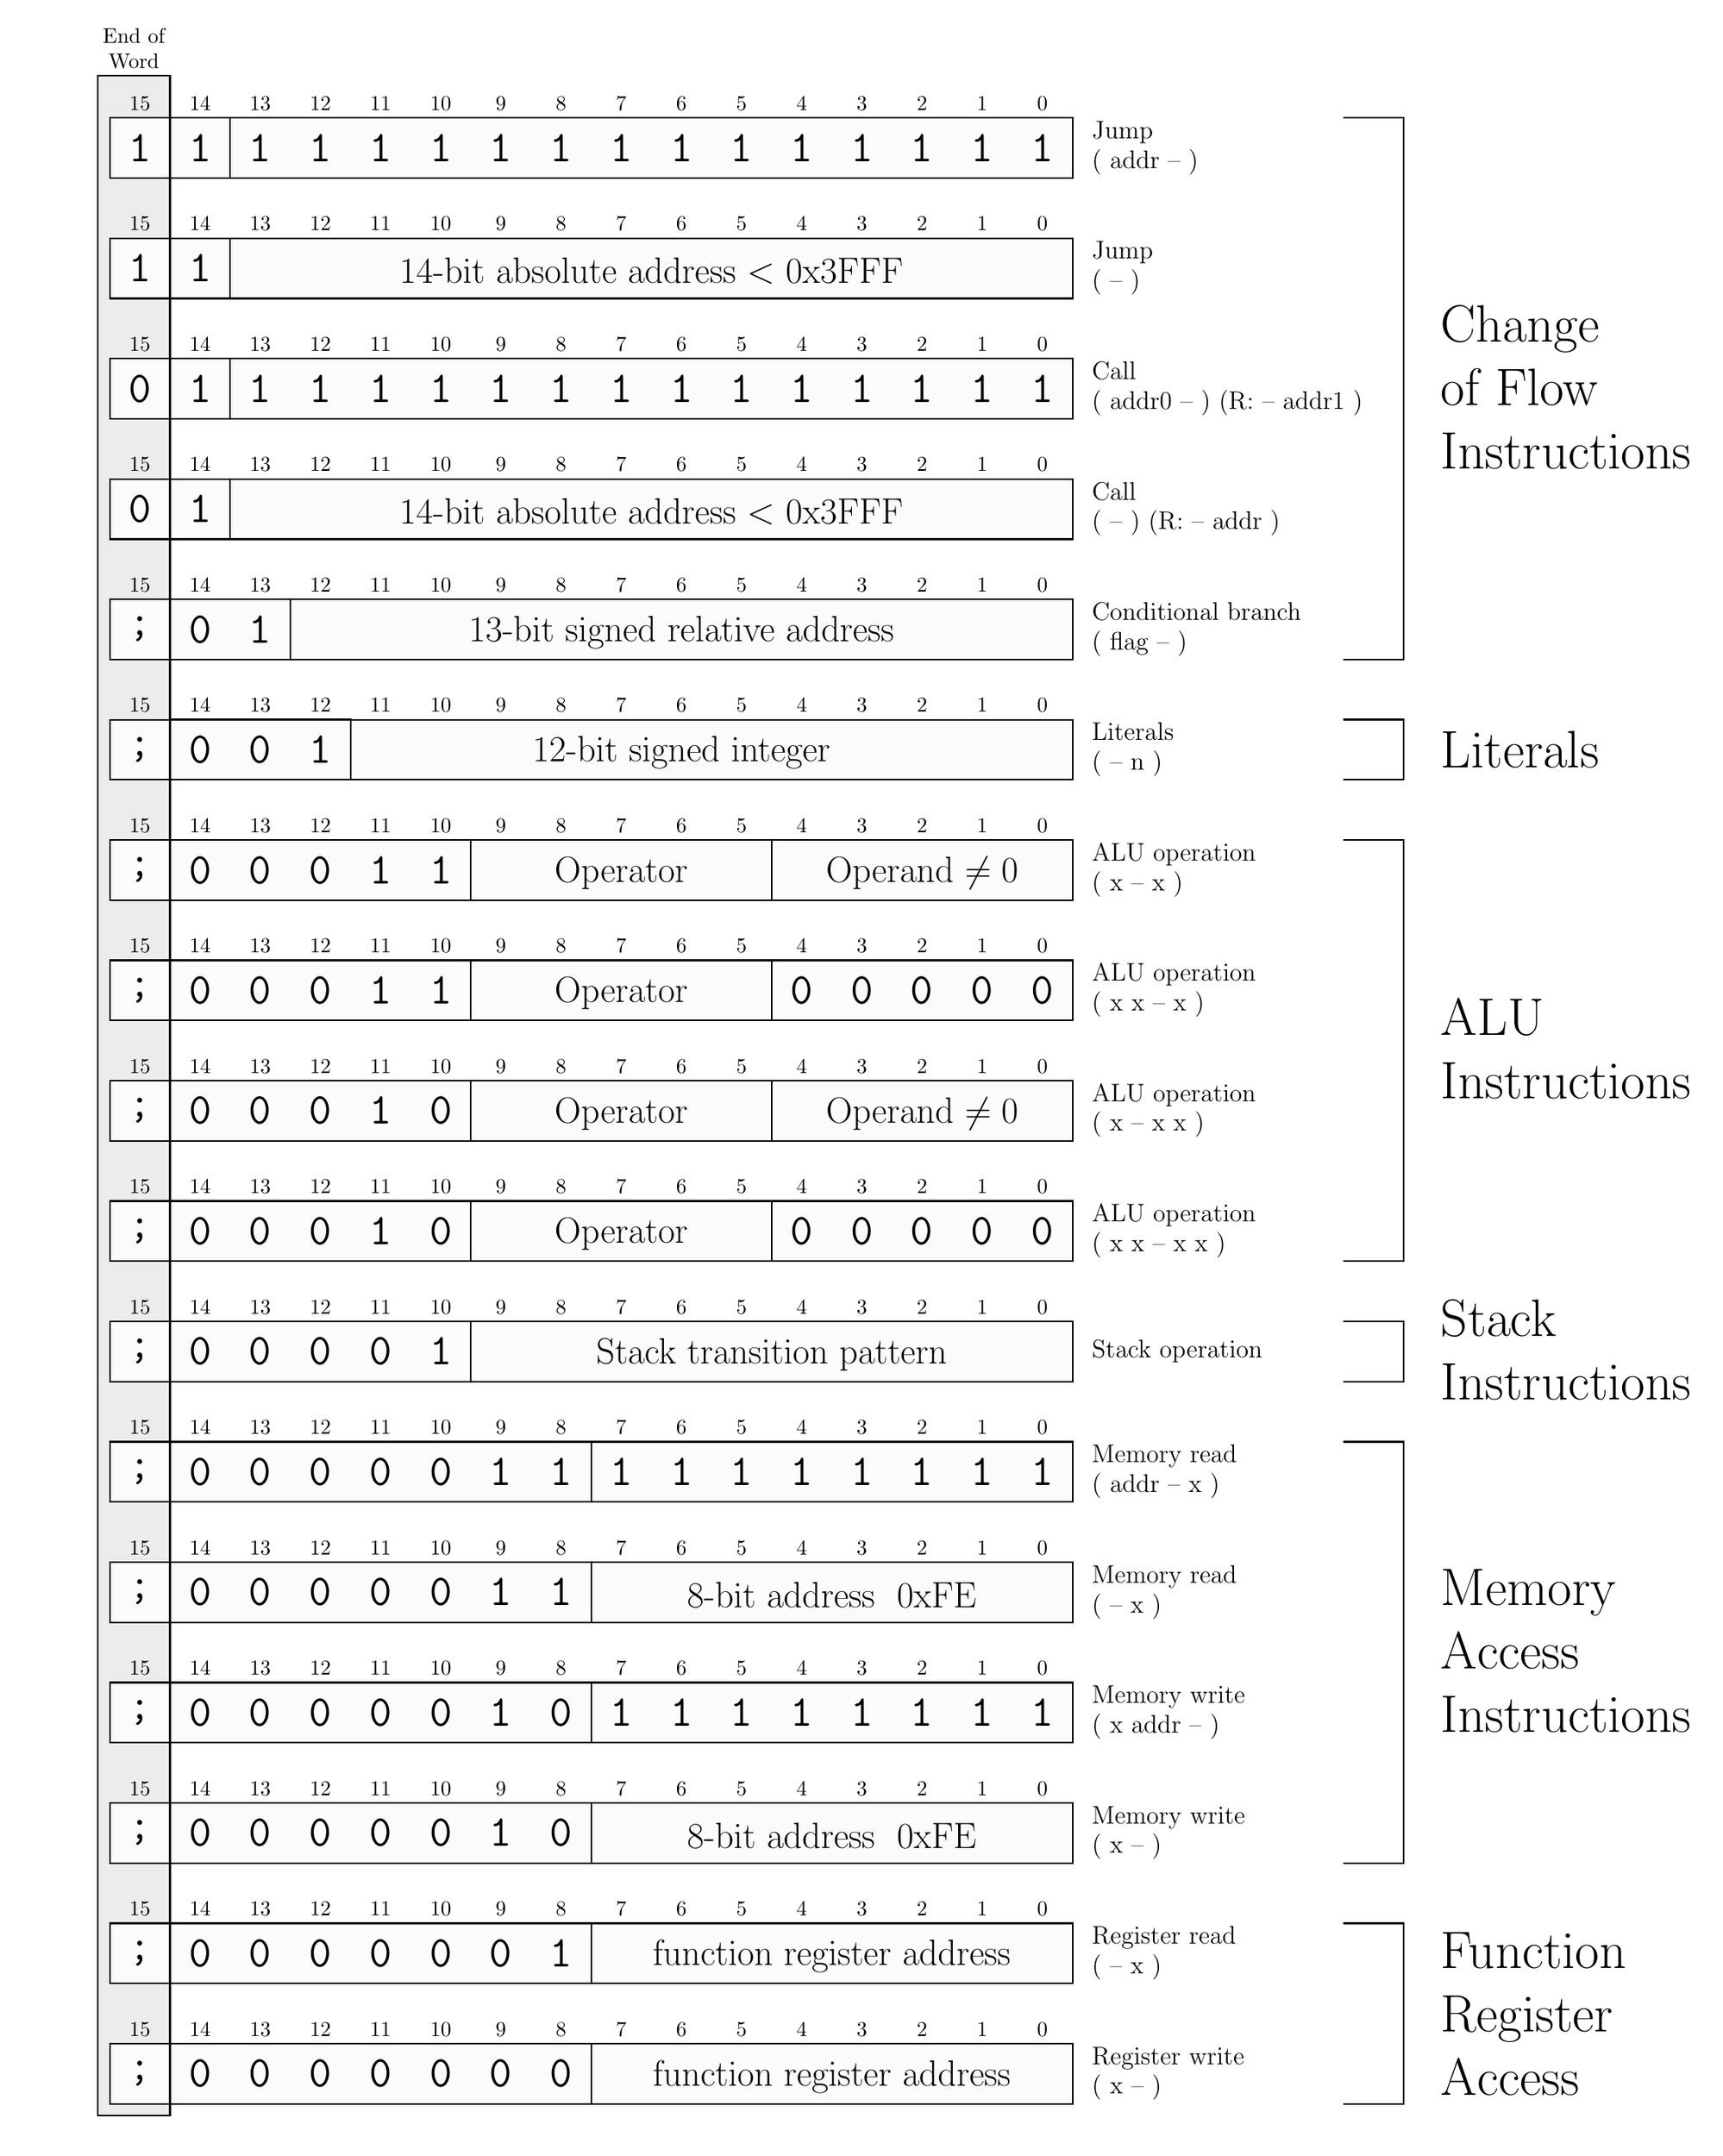
\begin{tikzpicture}
      
        %Instruction
        \newsavebox{\instruction}
        \savebox{\instruction}{
          \draw [thick, fill=gray!3] (0,0) rectangle (16,1);
          \draw [thick, fill=gray!3] (0,0) rectangle (1,1);
          \node [above] at (0.5,1)  {15};
          \node [above] at (1.5,1)  {14};
          \node [above] at (2.5,1)  {13};
          \node [above] at (3.5,1)  {12};
          \node [above] at (4.5,1)  {11};
          \node [above] at (5.5,1)  {10};
          \node [above] at (6.5,1)  {9};
          \node [above] at (7.5,1)  {8};
          \node [above] at (8.5,1)  {7};
          \node [above] at (9.5,1)  {6};
          \node [above] at (10.5,1) {5};
          \node [above] at (11.5,1) {4};
          \node [above] at (12.5,1) {3};
          \node [above] at (13.5,1) {2};
          \node [above] at (14.5,1) {1};
          \node [above] at (15.5,1) {0};
        };

        %Return bit
        \draw [thick, fill=gray!15] (0.8,0.3) rectangle (2,34.2);
        \node [above] at (1.4,34.2) {
          \begin{minipage}[c]{10em}
            \begin{center}
              End of\\
              Word
            \end{center}
          \end{minipage}};

        %Change of flow instructions
        \draw [thick] (21.5,33.5) -- (22.5,33.5) -- (22.5,24.5) -- (21.5,24.5);
        \node [right] at (23,28.5) {
          \begin{minipage}[l]{12em}
            \Huge{
              Change \\
              of Flow \\
              Instructions
            }
           \end{minipage}};

        %Jump
        \begin{scope}[shift={(1,32.5)}]
          \node at (0,0) {\usebox{\instruction}};
          \node         at (0.5,0.5)     {\huge{\texttt{1}}};
          \draw [thick] (1,0) rectangle  (2,1);
          \node         at (1.5,0.5)     {\huge{\texttt{1}}};
          \node         at (2.5,0.5)     {\huge{\texttt{1}}};
          \node         at (3.5,0.5)     {\huge{\texttt{1}}};
          \node         at (4.5,0.5)     {\huge{\texttt{1}}};
          \node         at (5.5,0.5)     {\huge{\texttt{1}}};
          \node         at (6.5,0.5)     {\huge{\texttt{1}}};
          \node         at (7.5,0.5)     {\huge{\texttt{1}}};
          \node         at (8.5,0.5)     {\huge{\texttt{1}}};
          \node         at (9.5,0.5)     {\huge{\texttt{1}}};
          \node         at (10.5,0.5)    {\huge{\texttt{1}}};
          \node         at (11.5,0.5)    {\huge{\texttt{1}}};
          \node         at (12.5,0.5)    {\huge{\texttt{1}}};
          \node         at (13.5,0.5)    {\huge{\texttt{1}}};
          \node         at (14.5,0.5)    {\huge{\texttt{1}}};
          \node         at (15.5,0.5)    {\huge{\texttt{1}}};
          \node [right] at (16.2,0.5) {
            \begin{minipage}[l]{14em}
              \large{
                Jump \\
                ( addr -- )
              }
          \end{minipage}};
        \end{scope}

        %Jump
        \begin{scope}[shift={(1,30.5)}]
          \node at (0,0) {\usebox{\instruction}};
          \node         at (0.5,0.5)     {\huge{\texttt{1}}};
          \draw [thick] (1,0) rectangle  (2,1);
          \node         at (1.5,0.5)     {\huge{\texttt{1}}};
          \node         at (9,0.45)      {\LARGE{14-bit absolute address $<$ 0x3FFF}};
          \node [right] at (16.2,0.5) {
            \begin{minipage}[l]{14em}
              \large{
                Jump \\
                ( -- )
              }
          \end{minipage}};
        \end{scope}

        %Call
        \begin{scope}[shift={(1,28.5)}]
          \node at (0,0) {\usebox{\instruction}};
          \node         at (0.5,0.5)     {\huge{\texttt{0}}};
          \draw [thick] (1,0) rectangle  (2,1);
          \node         at (1.5,0.5)     {\huge{\texttt{1}}};
          \node         at (2.5,0.5)     {\huge{\texttt{1}}};
          \node         at (3.5,0.5)     {\huge{\texttt{1}}};
          \node         at (4.5,0.5)     {\huge{\texttt{1}}};
          \node         at (5.5,0.5)     {\huge{\texttt{1}}};
          \node         at (6.5,0.5)     {\huge{\texttt{1}}};
          \node         at (7.5,0.5)     {\huge{\texttt{1}}};
          \node         at (8.5,0.5)     {\huge{\texttt{1}}};
          \node         at (9.5,0.5)     {\huge{\texttt{1}}};
          \node         at (10.5,0.5)    {\huge{\texttt{1}}};
          \node         at (11.5,0.5)    {\huge{\texttt{1}}};
          \node         at (12.5,0.5)    {\huge{\texttt{1}}};
          \node         at (13.5,0.5)    {\huge{\texttt{1}}};
          \node         at (14.5,0.5)    {\huge{\texttt{1}}};
          \node         at (15.5,0.5)    {\huge{\texttt{1}}};
          \node [right] at (16.2,0.5) {
            \begin{minipage}[l]{14em}
              \large{
                Call \\
                ( addr0 -- ) (R: -- addr1 )
              }
          \end{minipage}};
        \end{scope}

        %Call
        \begin{scope}[shift={(1,26.5)}]
          \node at (0,0) {\usebox{\instruction}};
          \node         at (0.5,0.5)     {\huge{\texttt{0}}};
          \draw [thick] (1,0) rectangle  (2,1);
          \node         at (1.5,0.5)     {\huge{\texttt{1}}};
          \node         at (9,0.45)      {\LARGE{14-bit absolute address $<$ 0x3FFF}};
          \node [right] at (16.2,0.5) {
            \begin{minipage}[l]{14em}
              \large{
                Call \\
                ( -- ) (R: -- addr )
              }
          \end{minipage}};
        \end{scope}

        %%Conditional Branch
        %\begin{scope}[shift={(1,26.5)}]
        %  \node at (0,0) {\usebox{\instruction}};
        %  \node         at (0.5,0.5)     {\huge{\texttt{;}}};
        %  \draw [thick] (1,0) rectangle  (3,1);
        %  \node         at (1.5,0.5)     {\huge{\texttt{0}}};
        %  \node         at (2.5,0.5)     {\huge{\texttt{1}}};
        %  \node         at (3.5,0.5)     {\huge{\texttt{1}}};
        %  \node         at (4.5,0.5)     {\huge{\texttt{1}}};
        %  \node         at (5.5,0.5)     {\huge{\texttt{1}}};
        %  \node         at (6.5,0.5)     {\huge{\texttt{1}}};
        %  \node         at (7.5,0.5)     {\huge{\texttt{1}}};
        %  \node         at (8.5,0.5)     {\huge{\texttt{1}}};
        %  \node         at (9.5,0.5)     {\huge{\texttt{1}}};
        %  \node         at (10.5,0.5)    {\huge{\texttt{1}}};
        %  \node         at (11.5,0.5)    {\huge{\texttt{1}}};
        %  \node         at (12.5,0.5)    {\huge{\texttt{1}}};
        %  \node         at (13.5,0.5)    {\huge{\texttt{1}}};
        %  \node         at (14.5,0.5)    {\huge{\texttt{1}}};
        %  \node         at (15.5,0.5)    {\huge{\texttt{1}}};
        %  \node [right] at (16.2,0.5) {
        %    \begin{minipage}[l]{14em}
        %      \large{
        %        Conditional branch \\
        %        ( flag addr -- )
        %      }
        %  \end{minipage}};
        %\end{scope}
        
        %Conditional Branch
        \begin{scope}[shift={(1,24.5)}]
          \node at (0,0) {\usebox{\instruction}};
          \node         at (0.5,0.5)     {\huge{\texttt{;}}};
          \draw [thick] (1,0) rectangle  (3,1);
          \node         at (1.5,0.5)     {\huge{\texttt{0}}};
          \node         at (2.5,0.5)     {\huge{\texttt{1}}};
          \node         at (9.5,0.45)    {\LARGE{13-bit signed relative address}};
          \node [right] at (16.2,0.5) {
            \begin{minipage}[l]{14em}
              \large{
                Conditional branch \\
               ( flag -- )
              }
          \end{minipage}};
        \end{scope}

        %Literal instructions
        \draw [thick] (21.5,22.5) -- (22.5,22.5) -- (22.5,23.5) -- (21.5,23.5);
        \node [right] at (23,23) {
          \begin{minipage}[l]{12em}
            \Huge{
              Literals
            }
           \end{minipage}};

        %Literal 
        \begin{scope}[shift={(1,22.5)}]
          \node at (0,0) {\usebox{\instruction}};
          \node         at (0.5,0.5)     {\huge{\texttt{;}}};
          \draw [thick] (1,0) rectangle  (4,1);
          \node         at (1.5,0.5)     {\huge{\texttt{0}}};
          \node         at (2.5,0.5)     {\huge{\texttt{0}}};
          \node         at (3.5,0.5)     {\huge{\texttt{1}}};
          \node         at (9.5,0.45)    {\LARGE{12-bit signed integer}};
          \node [right] at (16.2,0.5) {
            \begin{minipage}[l]{14em}
              \large{
                Literals \\
                ( -- n )
              }
          \end{minipage}};
        \end{scope}

        %ALU instructions
        \draw [thick] (21.5,21.5) -- (22.5,21.5) -- (22.5,14.5) -- (21.5,14.5);
        \node [right] at (23,17.5) {
          \begin{minipage}[l]{12em}
            \Huge{
              ALU \\
              Instructions
            }
          \end{minipage}};
  
        %ALU operation ( x -- x )
        \begin{scope}[shift={(1,20.5)}]
          \node at (0,0) {\usebox{\instruction}};
          \node         at (0.5,0.5)     {\huge{\texttt{;}}};
          \draw [thick] (1,0) rectangle  (6,1);
          \draw [thick] (6,0) rectangle (11,1); 
          \node         at (1.5,0.5)     {\huge{\texttt{0}}};
          \node         at (2.5,0.5)     {\huge{\texttt{0}}};
          \node         at (3.5,0.5)     {\huge{\texttt{0}}};
          \node         at (4.5,0.5)     {\huge{\texttt{1}}};
          \node         at (5.5,0.5)     {\huge{\texttt{1}}};
          \node         at (8.5,0.45)    {\LARGE{Operator}};
          \node         at (13.5,0.45)   {\LARGE{Operand $\neq 0$}};
          \node [right] at (16.2,0.5) {
            \begin{minipage}[l]{14em}
              \large{
                ALU operation \\
                ( x -- x )
              }
          \end{minipage}};
        \end{scope}

        %ALU operation ( x x -- x )
        \begin{scope}[shift={(1,18.5)}]
          \node at (0,0) {\usebox{\instruction}};
          \node         at (0.5,0.5)     {\huge{\texttt{;}}};
          \draw [thick] (1,0) rectangle  (6,1);
          \draw [thick] (6,0) rectangle (11,1); 
          \node         at (1.5,0.5)     {\huge{\texttt{0}}};
          \node         at (2.5,0.5)     {\huge{\texttt{0}}};
          \node         at (3.5,0.5)     {\huge{\texttt{0}}};
          \node         at (4.5,0.5)     {\huge{\texttt{1}}};
          \node         at (5.5,0.5)     {\huge{\texttt{1}}};
          \node         at (8.5,0.45)    {\LARGE{Operator}};
          \node         at (11.5,0.5)    {\huge{\texttt{0}}};   
          \node         at (12.5,0.5)    {\huge{\texttt{0}}};   
          \node         at (13.5,0.5)    {\huge{\texttt{0}}};   
          \node         at (14.5,0.5)    {\huge{\texttt{0}}};   
          \node         at (15.5,0.5)    {\huge{\texttt{0}}};   
          \node [right] at (16.2,0.5) {
            \begin{minipage}[l]{14em}
              \large{
                ALU operation \\
                ( x x -- x )
              }
          \end{minipage}};
        \end{scope}
               
        %ALU operation ( x -- x x )
        \begin{scope}[shift={(1,16.5)}]
          \node at (0,0) {\usebox{\instruction}};
          \node         at (0.5,0.5)     {\huge{\texttt{;}}};
          \draw [thick] (1,0) rectangle  (6,1);
          \draw [thick] (6,0) rectangle (11,1); 
          \node         at (1.5,0.5)     {\huge{\texttt{0}}};
          \node         at (2.5,0.5)     {\huge{\texttt{0}}};
          \node         at (3.5,0.5)     {\huge{\texttt{0}}};
          \node         at (4.5,0.5)     {\huge{\texttt{1}}};
          \node         at (5.5,0.5)     {\huge{\texttt{0}}};
          \node         at (8.5,0.45)    {\LARGE{Operator}};
          \node         at (13.5,0.45)   {\LARGE{Operand $\neq 0$}};
          \node [right] at (16.2,0.5) {
            \begin{minipage}[l]{14em}
              \large{
                ALU operation \\
                ( x -- x x )
              }
          \end{minipage}};
        \end{scope}

        %ALU operation ( x x -- x x )
        \begin{scope}[shift={(1,14.5)}]
          \node at (0,0) {\usebox{\instruction}};
          \node         at (0.5,0.5)     {\huge{\texttt{;}}};
          \draw [thick] (1,0) rectangle  (6,1);
          \draw [thick] (6,0) rectangle (11,1); 
          \node         at (1.5,0.5)     {\huge{\texttt{0}}};
          \node         at (2.5,0.5)     {\huge{\texttt{0}}};
          \node         at (3.5,0.5)     {\huge{\texttt{0}}};
          \node         at (4.5,0.5)     {\huge{\texttt{1}}};
          \node         at (5.5,0.5)     {\huge{\texttt{0}}};
          \node         at (8.5,0.45)    {\LARGE{Operator}};
          \node         at (11.5,0.5)    {\huge{\texttt{0}}};   
          \node         at (12.5,0.5)    {\huge{\texttt{0}}};   
          \node         at (13.5,0.5)    {\huge{\texttt{0}}};   
          \node         at (14.5,0.5)    {\huge{\texttt{0}}};   
          \node         at (15.5,0.5)    {\huge{\texttt{0}}};   
          \node [right] at (16.2,0.5) {
            \begin{minipage}[l]{14em}
              \large{
                ALU operation \\
                ( x x -- x x )
              }
          \end{minipage}};
        \end{scope}

        %Stack instructions
        \draw [thick] (21.5,12.5) -- (22.5,12.5) -- (22.5,13.5) -- (21.5,13.5);
        \node [right] at (23,12.5) {
          \begin{minipage}[l]{12em}
            \Huge{
              Stack \\
              Instructions
            }
           \end{minipage}};

        %Stack operation 
        \begin{scope}[shift={(1,12.5)}]
          \node at (0,0) {\usebox{\instruction}};
          \node         at (0.5,0.5)     {\huge{\texttt{;}}};
          \draw [thick] (1,0) rectangle (6,1); 
          \node         at (1.5,0.5)     {\huge{\texttt{0}}};
          \node         at (2.5,0.5)     {\huge{\texttt{0}}};
          \node         at (3.5,0.5)     {\huge{\texttt{0}}};
          \node         at (4.5,0.5)     {\huge{\texttt{0}}};   
          \node         at (5.5,0.5)     {\huge{\texttt{1}}};   
          \node         at (11,0.45)     {\LARGE{Stack transition pattern}};
          \node [right] at (16.2,0.5) {
            \begin{minipage}[l]{14em}
              \large{
                Stack operation
              }
          \end{minipage}};
        \end{scope}

        %Memory access instructions
        \draw [thick] (21.5,11.5) -- (22.5,11.5) -- (22.5,4.5) -- (21.5,4.5);
        \node [right] at (23,7.5) {
          \begin{minipage}[l]{12em}
            \Huge{
              Memory \\
              Access \\
              Instructions
            }
           \end{minipage}};

        %Memory read
        \begin{scope}[shift={(1,10.5)}]
          \node at (0,0) {\usebox{\instruction}};
          \node         at (0.5,0.5)     {\huge{\texttt{;}}};
          \draw [thick] (1,0) rectangle  (8,1);
          \node         at (1.5,0.5)     {\huge{\texttt{0}}};
          \node         at (2.5,0.5)     {\huge{\texttt{0}}};
          \node         at (3.5,0.5)     {\huge{\texttt{0}}};
          \node         at (4.5,0.5)     {\huge{\texttt{0}}};
          \node         at (5.5,0.5)     {\huge{\texttt{0}}};
          \node         at (6.5,0.5)     {\huge{\texttt{1}}};
          \node         at (7.5,0.5)     {\huge{\texttt{1}}};
          \node         at (8.5,0.5)     {\huge{\texttt{1}}};
          \node         at (9.5,0.5)     {\huge{\texttt{1}}};
          \node         at (10.5,0.5)    {\huge{\texttt{1}}};
          \node         at (11.5,0.5)    {\huge{\texttt{1}}};
          \node         at (12.5,0.5)    {\huge{\texttt{1}}};
          \node         at (13.5,0.5)    {\huge{\texttt{1}}};
          \node         at (14.5,0.5)    {\huge{\texttt{1}}};
          \node         at (15.5,0.5)    {\huge{\texttt{1}}};
          \node [right] at (16.2,0.5) {
           \begin{minipage}[l]{14em}
              \large{
                Memory read \\
                ( addr -- x )
              }
          \end{minipage}};
        \end{scope}

        %Memory read
        \begin{scope}[shift={(1,8.5)}]
          \node at (0,0) {\usebox{\instruction}};
          \node         at (0.5,0.5)     {\huge{\texttt{;}}};
          \draw [thick] (1,0) rectangle  (8,1);
          \node         at (1.5,0.5)     {\huge{\texttt{0}}};
          \node         at (2.5,0.5)     {\huge{\texttt{0}}};
          \node         at (3.5,0.5)     {\huge{\texttt{0}}};
          \node         at (4.5,0.5)     {\huge{\texttt{0}}};
          \node         at (5.5,0.5)     {\huge{\texttt{0}}};
          \node         at (6.5,0.5)     {\huge{\texttt{1}}};
          \node         at (7.5,0.5)     {\huge{\texttt{1}}};
          \node         at (12,0.45)    {\LARGE{8-bit address $\leqslant$ 0xFE}};
          \node [right] at (16.2,0.5) {
           \begin{minipage}[l]{14em}
              \large{
                Memory read \\
                ( -- x )
              }
          \end{minipage}};
        \end{scope}


        %Memory write
        \begin{scope}[shift={(1,6.5)}]
          \node at (0,0) {\usebox{\instruction}};
          \node         at (0.5,0.5)     {\huge{\texttt{;}}};
          \draw [thick] (1,0) rectangle  (8,1);
          \node         at (1.5,0.5)     {\huge{\texttt{0}}};
          \node         at (2.5,0.5)     {\huge{\texttt{0}}};
          \node         at (3.5,0.5)     {\huge{\texttt{0}}};
          \node         at (4.5,0.5)     {\huge{\texttt{0}}};
          \node         at (5.5,0.5)     {\huge{\texttt{0}}};
          \node         at (6.5,0.5)     {\huge{\texttt{1}}};
          \node         at (7.5,0.5)     {\huge{\texttt{0}}};
          \node         at (8.5,0.5)     {\huge{\texttt{1}}};
          \node         at (9.5,0.5)     {\huge{\texttt{1}}};
          \node         at (10.5,0.5)    {\huge{\texttt{1}}};
          \node         at (11.5,0.5)    {\huge{\texttt{1}}};
          \node         at (12.5,0.5)    {\huge{\texttt{1}}};
          \node         at (13.5,0.5)    {\huge{\texttt{1}}};
          \node         at (14.5,0.5)    {\huge{\texttt{1}}};
          \node         at (15.5,0.5)    {\huge{\texttt{1}}};
          \node [right] at (16.2,0.5) {
           \begin{minipage}[l]{14em}
              \large{
                Memory write \\
                ( x addr -- )
              }
          \end{minipage}};
        \end{scope}

        %Memory write
        \begin{scope}[shift={(1,4.5)}]
          \node at (0,0) {\usebox{\instruction}};
          \node         at (0.5,0.5)     {\huge{\texttt{;}}};
          \draw [thick] (1,0) rectangle  (8,1);
          \node         at (1.5,0.5)     {\huge{\texttt{0}}};
          \node         at (2.5,0.5)     {\huge{\texttt{0}}};
          \node         at (3.5,0.5)     {\huge{\texttt{0}}};
          \node         at (4.5,0.5)     {\huge{\texttt{0}}};
          \node         at (5.5,0.5)     {\huge{\texttt{0}}};
          \node         at (6.5,0.5)     {\huge{\texttt{1}}};
          \node         at (7.5,0.5)     {\huge{\texttt{0}}};
          \node         at (12,0.45)     {\LARGE{8-bit address $\leqslant$ 0xFE}};
          \node [right] at (16.2,0.5) {
           \begin{minipage}[l]{14em}
              \large{
                Memory write \\
                ( x -- )
              }
          \end{minipage}};
        \end{scope}

        %Function register access
        \draw [thick] (21.5,3.5) -- (22.5,3.5) -- (22.5,0.5) -- (21.5,0.5);
        \node [right] at (23,2) {
          \begin{minipage}[l]{12em}
            \Huge{
              Function \\
              Register \\
              Access
            }
           \end{minipage}};
       
        %Function register read
        \begin{scope}[shift={(1,2.5)}]
          \node at (0,0) {\usebox{\instruction}};
          \node         at (0.5,0.5)     {\huge{\texttt{;}}};
          \draw [thick] (1,0) rectangle  (8,1);
          \node         at (1.5,0.5)     {\huge{\texttt{0}}};
          \node         at (2.5,0.5)     {\huge{\texttt{0}}};
          \node         at (3.5,0.5)     {\huge{\texttt{0}}};
          \node         at (4.5,0.5)     {\huge{\texttt{0}}};
          \node         at (5.5,0.5)     {\huge{\texttt{0}}};
          \node         at (6.5,0.5)     {\huge{\texttt{0}}};
          \node         at (7.5,0.5)     {\huge{\texttt{1}}};
          \node         at (12,0.45)     {\LARGE{function register address}};
          \node [right] at (16.2,0.5) {
           \begin{minipage}[l]{14em}
              \large{
                Register read \\
                ( -- x )
              }
          \end{minipage}};
        \end{scope}

        %Function register write
        \begin{scope}[shift={(1,0.5)}]
          \node at (0,0) {\usebox{\instruction}};
          \node         at (0.5,0.5)     {\huge{\texttt{;}}};
          \draw [thick] (1,0) rectangle  (8,1);
          \node         at (1.5,0.5)     {\huge{\texttt{0}}};
          \node         at (2.5,0.5)     {\huge{\texttt{0}}};
          \node         at (3.5,0.5)     {\huge{\texttt{0}}};
          \node         at (4.5,0.5)     {\huge{\texttt{0}}};
          \node         at (5.5,0.5)     {\huge{\texttt{0}}};
          \node         at (6.5,0.5)     {\huge{\texttt{0}}};
          \node         at (7.5,0.5)     {\huge{\texttt{0}}};
          \node         at (12,0.45)     {\LARGE{function register address}};
          \node [right] at (16.2,0.5) {
           \begin{minipage}[l]{14em}
              \large{
                Register write  \\
                ( x -- )
              }
          \end{minipage}};
        \end{scope}
        
      \end{tikzpicture}
    }
  }
  \caption{Instruction encoding}
  \label{opcodes:encoding}
  %\end{center}
\end{figure}

\subsection{Return from a Call (\texttt{;})}
\label{opcodes:rtc}

Rather than  providing a dedicated instruction to end the execution of 
word in Forth and to return the caller's program flow, the N1 allows
to perform this operation in parallel to the execution of any of its
instructions. Each \gls{opcode} contains a bit (bit 15) to indicate, that the
current instruction is the last operation of the current word. If this bit
is set, the program flow will resume at the calling word as soon as the
operationis performed.

As shown in \figref{opcodes:encoding}, bit 15 is also distinction between the
encoding of \gls{jump} and of \gls{call} instructions.
Considering that the last \gls{call} in a word definition can be optimized
to a \gls{jump}, bit 15 can be regarded
as the termination bit for \gls{call} instructions as well.

For a Forth compiler, this means that the semi-colon (\texttt{\gls{semicolon}})
always translates to setting bit 15 of the last instruction.

\subsection{Jump Instructions}
\label{opcodes:jump}

\Gls{jump} instructions transfer the program flow to any address
location within the supported 128KB program space. \Gls{jump} instructions consume an absolute
destination address which can either be placed on the top of the \gls{ps} or encoded
into the opcode of the instruction (only for destination addresses $<$ 0x3FFF).

\subsection{Call Instructions}
\label{opcodes:call}

\Gls{call} instructions temporarily transfer the program flow to any address
location within the supported 128KB program space, while pushing a return address onto
the \gls{rs}. \Gls{call} instructions consume an absolute
destination address which can either be placed on the top of the \Gls{ps} or encoded
into the opcode of the instruction (only for destination addresses $<$ 0x3FFF).

\subsection{Conditional Branches}
\label{opcodes:branch}

\Glspl{branch} invoke a change of program flow depending on the argument at the \glslink{tos}{top}
of the \gls{ps}.
If it is zero, then the branch is taken.
The branch destination is a \glslink{reladr}{relative address}, encoded into the opcode
of the instruction in the range of $\pm$ 8KB.
A relative address of value zero points to the istruction following the \glspl{branch}.

\subsection{Literals}
\label{opcodes:literal}

Signed integer \glspl{literal} of 12-bit length can be pushed onto the \gls{ps} within
a single instruction. For larger integers a supplemental \gls{alu} instruction is required.
(see encoding \texttt{11100} in \tabref{opcodes:alu:operators})

\subsection{ALU Instructions}
\label{opcodes:alu}
\Gls{alu} instructions perform an operation on two \gls{cell} values, resulting in a new double 
\gls{cell} value. The result can either be placed entirely onto the \gls{ps}, or truncated, discarding
the most significant \gls{cell}. The first operand is always taken from the \gls{ps}. The second operand can
either be taken from the \gls{ps} or encoded into the opcode of the instruction. In the latter case,
the interpretation of the embedded 5-bit value depends on the operation. The \glslink{immop}{immediate} value is
interpreted as either an unsigned ($uimm$), a sign extended ($simm$), or an offsetted ($oimm$) integer value:

\begin{align*}
  uimm &= \text{opcode[4:0]}                                     \\
  simm &= \begin{cases}
            \text{opcode[4:0]},      &\text{if opcode[4:0]} < 16 \\
            \text{opcode[4:0]} - 32, &\text{if opcode[4:0]} \ge 16
          \end{cases}                                            \\
  oimm &= \text{opcode[4:0]} - 16
\end{align*}

\tabref{opcodes:alu:operators} lists the supported \gls{alu} operations.

\begingroup
\setlength{\LTleft}{-20cm plus -1fill}
\setlength{\LTright}{\LTleft}
\begin{center}
  \rowcolors{1}{gray!12}{white}                                         %set alternating row color
  \begin{longtable}{|c|c|c|c|}
    \rowcolor{white}
    \caption{\Gls{alu} operations}
    \label{opcodes:alu:operators} \\
    %Header
    \hline                                     
    \rowcolor{gray!25}
    \multicolumn{1}{|c|}{\textbf{\rule{0pt}{2.5ex}Encoding}}     &  
    \multicolumn{1}{c|}{\textbf{\rule{0pt}{2.5ex}Operation}}     &
    \multicolumn{1}{c|}{\textbf{\rule{0pt}{2.5ex}( x1 -- d )}}   &
    \multicolumn{1}{c|}{\textbf{\rule{0pt}{2.5ex}( x1 x2 -- d ) }} \\
    \hline
    \endhead                               
    %Footers
    \hline
    \rowcolor{white}
    \multicolumn{4}{r}{\tiny{...continued}} \\
    \endfoot
    \hline
    \endlastfoot

    %Adder operations
    %---------------------------------
    %Sum
    \texttt{00000}                       &
    Sum                                  &
    $uimm$ $+$ x1                        &
    x1 $+$ x2                            \\ \hline
    
    %Sum
    \texttt{00001}                       &
    Absolute value                       &
    $oimm$ $+$ ABS(x1)                   &
    x1 $+$ ABS(x2)                       \\ \hline
                                           
    %Difference                            
    \texttt{00010}                       &
    Difference                           &
    x1 $-$ $uimm$                        &
    x2 $-$ x1                            \\ \hline

    %Difference                            
    \texttt{00011}                       &
    Difference                           &
    $oimm$ $-$ x1                        &
    x1 $-$ x2                            \\ \hline
    %---------------------------------
    
    %MAX/MIN values
    %---------------------------------
    %Unsigned MIN value
    \texttt{00100}                       &
    Unsigned minimum value               &
    UMIN($uimm$, x1)                     &
    UMIN(x1, x2)                         \\ \hline
    
    %Signed MAX value
    \texttt{00101}                       &
    Signed maximum value                 &
    MAX($oimm$, x1)                      &
    MAX(x1, x2)                          \\ \hline
                                           
    %Unsigned MAX value                            
    \texttt{00110}                       &
    Unsigned maximum value               &
    UMAX($uimm$, x1)                     &
    UMAX(x1, x2)                         \\ \hline

    %Signed MIN value                            
    \texttt{00111}                       &
    Signed minimum value                 &
    MIN($oimm$, x1)                      &
    MIN(x1, x2)                          \\ \hline
    %---------------------------------

    %Equals comparisons
    %---------------------------------
    %Equals                    
    \texttt{01000}                       &
    Equals comparison                    &
    $uimm$ $=$ x1?                       &
    x1 $=$ x2?                           \\ \hline

    %Equals
    \texttt{01001}                       &
    Equals comparison                    &
    $oimm$ $=$ x1?                       &
    x1 $=$ x2?                           \\ \hline

    %Not-Equals                     
    \texttt{01010}                       &
    Not-equals comparison                &
    $uimm$ $\ne$ x1?                     &
    x1 $\ne$ x2?                         \\ \hline

    %Not-Eqials
    \texttt{01011}                       &
    Not-equals comparison                &
    $oimm$ $\ne$ x1?                     &
    x1 $\ne$ x2?                         \\ \hline
    %---------------------------------

    %Greater/lower-than comparisons
    %---------------------------------
    %Unsigned greater-than                     
    \texttt{01100}                       &
    Unsigned greater-than comparison     &
    $uimm$ $>$ x1?                       &
    x1 $>$ x2?                           \\ \hline

    %Signed lower-than
    \texttt{01101}                       &
    Signed lower-than comparison         &
    $oimm$ $<$ x1?                       &
    x1 $<$ x2?                           \\ \hline

    %Unsigned lower-than                     
    \texttt{01110}                       &
    Unsigned lower-than comparison       &
    $uimm$ $<$ x1?                       &
    x1 $<$ x2?                           \\ \hline

    %Signed greater-than
    \texttt{01111}                       &
    Signed greater-than                  &
    $oimm$ $>$ x1?                       &
    x1 $>$ x2?                           \\ \hline
    %---------------------------------
      
    %Multiplier operations             
    %---------------------------------
    %Unsigned product                  
      \texttt{10000}                     &
      Unsigned product                   &
      $uimm$ $*$ x1                      &
      x1 $*$ x2                          \\ \hline
                                         
    %Unsigned product                      
      \texttt{10001}                     &
      Unsigned product                   &
      $simm$ $*$ x1                      &
      x1 $*$ x2                          \\ \hline
                                         
    %Signed product                  
      \texttt{10010}                     &
      Signed product                     &
      $uimm$ $*$ x1                      &
      x1 $*$ x2                          \\ \hline
                                         
    %Signed product                      
      \texttt{10011}                     &
      Signed product                     &
      $simm$ $*$ x1                      &
      x1 $*$ x2                          \\ \hline
    %---------------------------------
                                         
    %Bitwise logic operations          
    %---------------------------------
   %AND                               
      \texttt{10100}                     &
      Logic AND                          &
      $simm$ $\land$ x1                  &
      x1 $\land$ x2                      \\ \hline
                                         
    %XOR                                 
      \texttt{10101}                     &
      Logic XOR                          &
      $simm$ $\oplus$ x1                 &
      x1 $\oplus$ x2                     \\ \hline
                                         
    %OR                                  
      \texttt{10110}                     &
      Logic OR                           &
      $uimm$ $\lor$ x1                   &
      x1 $\lor$ x2                       \\ \hline
                                         
    %Reserved                            
      \texttt{10111}                     &
      \multicolumn{3}{c|}{Reserved}      \\ \hline
    %---------------------------------

    %Shift operations             
    %---------------------------------
    %Logic right shift
      \texttt{11000}                     &
      Logic right shift                  &
      x1 $\gg$ $uimm$                    &
      x1 $\gg$ x2                        \\ \hline
                                         
    %Logic left shift                    
      \texttt{11001}                     &
      Logic left shift                   &
      x1 $\ll$ $uimm$                    &
      x1 $\ll$ x2                        \\ \hline
                                         
    %Arithmetic right shift              
      \texttt{11010}                     &                      
      Arithmetic right shift             &
      x1 $\gg$ $uimm$                    &
      x1 $\gg$ x2                        \\ \hline

    %Reserved                          
      \texttt{11011}                     &
      \multicolumn{3}{c|}{Reserved}      \\ \hline
    %---------------------------------

    %Special operations             
    %---------------------------------
    %Literal value
      \texttt{11100}                     &
      Set upper bits of a literal value  &
      {$simm$, x1[11:0]}                 &   
      {$simm$, x2[11:0]}                 \\ \hline
 
    %Reserved                          
      \texttt{11101}                     &
      \multicolumn{3}{c|}{Reserved}      \\ \hline


    %Reserved                          
      \texttt{11110}                     &
      \multicolumn{3}{c|}{Reserved}      \\ \hline

    %Reserved                          
      \texttt{11111}                     &
      \multicolumn{3}{c|}{Reserved}      \\ \hline
    %---------------------------------
    
  \end{longtable}
\end{center}  
\endgroup

\subsection{Stack Instructions}
\label{opcodes:stack}

The N1's stack instruction aims at efficiently implementing common stack operations
of the \Gls{forth} language, while only implementing the essential data paths, which are
needed for plain push and pull operations.

The opcode of the stack instruction contains a 10-bit field to specify a transition
pattern of the upper \glspl{cell} of the \gls{ps} and the \gls{rs}. 
The structure transition pattern is shown in \figref{opcodes:stack:transpat}.
    
\begin{figure}[!h]
  %\begin{center}
  \makebox[\textwidth][c]{
    \scalebox{0.8} {
      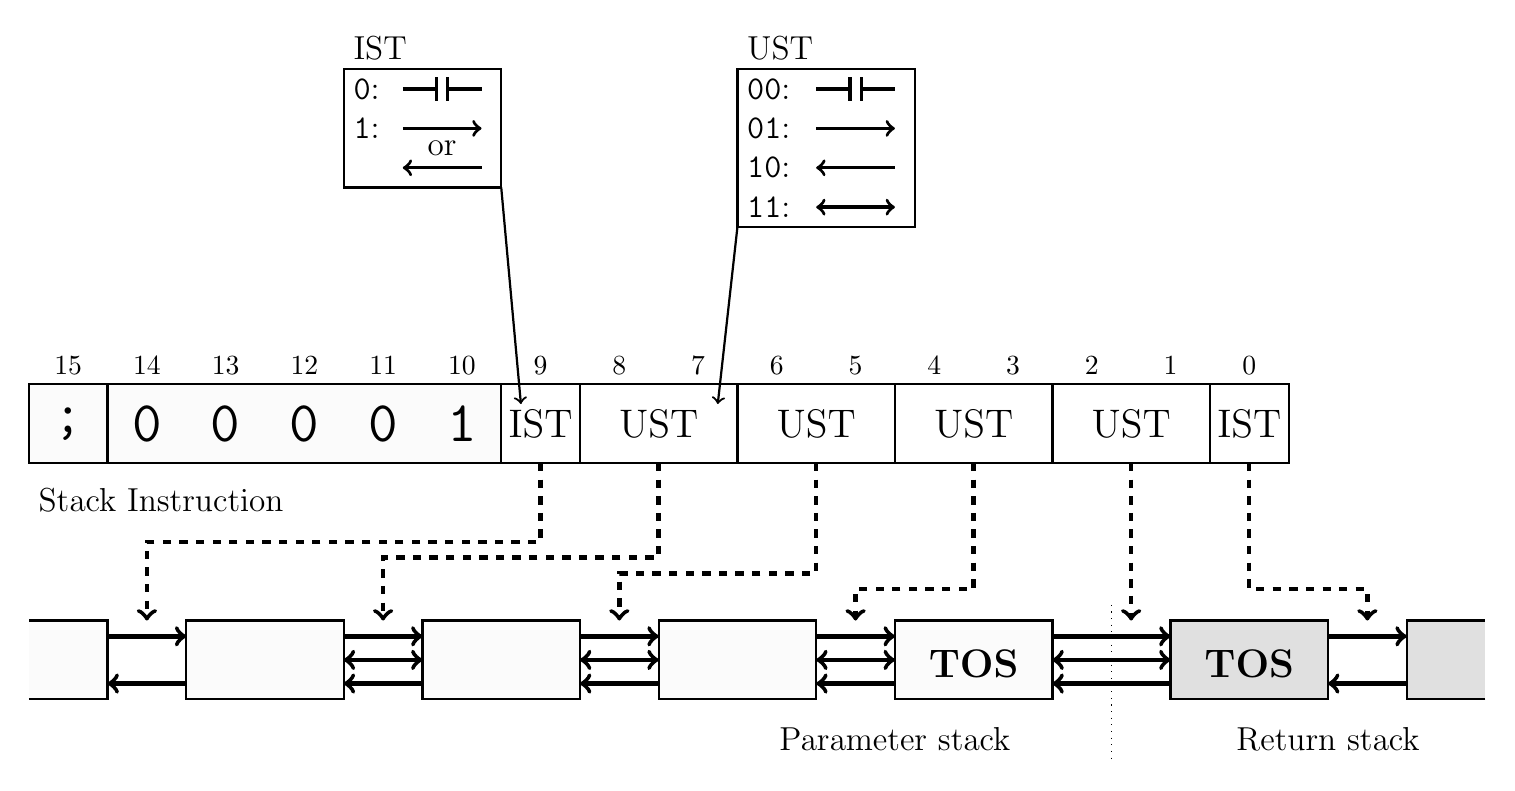
\begin{tikzpicture}

        %Stack instruction
        \draw [thick, fill=gray!3]  (1,4) rectangle (17,5);
        \draw [thick]               (1,4) rectangle  (2,5);
        \draw [thick]               (2,4) rectangle  (7,5); 
        \draw [thick, fill=white]   (7,4) rectangle  (8,5); 
        \draw [thick, fill=white]   (8,4) rectangle (10,5); 
        \draw [thick, fill=white]  (10,4) rectangle (12,5); 
        \draw [thick, fill=white]  (12,4) rectangle (14,5); 
        \draw [thick, fill=white]  (14,4) rectangle (16,5); 
        \draw [thick, fill=white]  (16,4) rectangle (17,5); 
  
        \node [above] at  (1.5,5) {15};
        \node [above] at  (2.5,5) {14};
        \node [above] at  (3.5,5) {13};
        \node [above] at  (4.5,5) {12};
        \node [above] at  (5.5,5) {11};
        \node [above] at  (6.5,5) {10};
        \node [above] at  (7.5,5) {9};
        \node [above] at  (8.5,5) {8};
        \node [above] at  (9.5,5) {7};
        \node [above] at (10.5,5) {6};
        \node [above] at (11.5,5) {5};
        \node [above] at (12.5,5) {4};
        \node [above] at (13.5,5) {3};
        \node [above] at (14.5,5) {2};
        \node [above] at (15.5,5) {1};
        \node [above] at (16.5,5) {0};

        \node         at (1.5,4.5)     {\huge{\texttt{;}}};
        \node         at (2.5,4.5)     {\huge{\texttt{0}}};
        \node         at (3.5,4.5)     {\huge{\texttt{0}}};
        \node         at (4.5,4.5)     {\huge{\texttt{0}}};
        \node         at (5.5,4.5)     {\huge{\texttt{0}}};   
        \node         at (6.5,4.5)     {\huge{\texttt{1}}};   

        \node         at (7.5,4.5)     {\Large{IST}};   
        \node         at (9,4.5)       {\Large{UST}};   
        \node         at (11,4.5)      {\Large{UST}};   
        \node         at (13,4.5)      {\Large{UST}};   
        \node         at (15,4.5)      {\Large{UST}};   
        \node         at (16.5,4.5)    {\Large{IST}};   
        
        \node [below right] at (1,3.8) {\large{Stack Instruction}};

        %IST field description
        \draw [thick]               (5,7.5) rectangle (7,9);
        \node [above right] at      (5,9) {\large{IST}};
        \node [right] at (5,8.75)    {\large{\texttt{0}:}};   
        \node [right] at (5,8.25)    {\large{\texttt{1}:}};

        \draw [very thick, -|]     (5.75,8.75)  -- (6.2,8.75);
        \draw [very thick, |-]     (6.3,8.75)   -- (6.75,8.75);
        \draw [very thick, ->]     (5.75,8.25)  -- (6.75,8.25);
        \node at (6.25,8)          {\large{or}};
        \draw [very thick, <-]     (5.75,7.75)  -- (6.75,7.75);         
        \draw [thick, ->]          (7,7.5)   --  (7.25,4.75);
       
        %UST field description
        \draw [thick]               (10,7) rectangle  (12.25,9);
        \node [above right] at      (10,9) {\large{UST}};
        \node [right] at (10,8.75) {\large{\texttt{00}:}};   
        \node [right] at (10,8.25) {\large{\texttt{01}:}};   
        \node [right] at (10,7.75) {\large{\texttt{10}:}};   
        \node [right] at (10,7.25) {\large{\texttt{11}:}};   

        \draw [very thick, -|]     (11,8.75)    -- (11.45,8.75);
        \draw [very thick, |-]     (11.55,8.75) -- (12,8.75);
        \draw [very thick, ->]     (11,8.25)    --  (12,8.25);
        \draw [very thick, <-]     (11,7.75)    --  (12,7.75);
        \draw [very thick, <->]    (11,7.25)    --  (12,7.25);         
        \draw [thick, ->]          (10,7)       --  (9.75,4.75);

        %Bit field association
        \draw [ultra thick, dashed, ->]  (7.5,4)  -- (7.5,3)    -- (2.5,3)    -- (2.5,2);
        \draw [ultra thick, dashed, ->]  (9,4)    -- (9,2.8)    -- (5.5,2.8)  -- (5.5,2);
        \draw [ultra thick, dashed, ->]  (11,4)   -- (11,2.6)   -- (8.5,2.6)  -- (8.5,2);
        \draw [ultra thick, dashed, ->]  (13,4)   -- (13,2.4)   -- (11.5,2.4) -- (11.5,2);
        \draw [ultra thick, dashed, ->]  (15,4)   -- (15,2);
        \draw [ultra thick, dashed, ->]  (16.5,4) -- (16.5,2.4) -- (18,2.4) -- (18,2);
    
        %Lower parameter stack
        \draw [thick, fill=gray!3]  (1,1) -- (2,1) -- (2,2) -- (1,2);
        \draw [ultra thick, ->]     (2,1.8) --  (3,1.8);
        \draw [ultra thick, <-]     (2,1.2) --  (3,1.2);         
       
        %Upper parameter stack
        \draw [thick, fill=gray!3]  (3,1) rectangle  (5,2);
        \draw [ultra thick, ->]     (5,1.8) --  (6,1.8);
        \draw [ultra thick, <->]    (5,1.5) --  (6,1.5);
        \draw [ultra thick, <-]     (5,1.2) --  (6,1.2);         

        \draw [thick, fill=gray!3]  (6,1) rectangle  (8,2);
        \draw [ultra thick, ->]     (8,1.8) --  (9,1.8);
        \draw [ultra thick, <->]    (8,1.5) --  (9,1.5);
        \draw [ultra thick, <-]     (8,1.2) --  (9,1.2);         

        \draw [thick, fill=gray!3]  (9,1) rectangle  (11,2);
        \draw [ultra thick, ->]     (11,1.8) --  (12,1.8);
        \draw [ultra thick, <->]    (11,1.5) --  (12,1.5);
        \draw [ultra thick, <-]     (11,1.2) --  (12,1.2);         

        \draw [thick, fill=gray!3]  (12,1) rectangle  (14,2);
        \node at (13,1.45)          {\Large{\textbf{TOS}}};        
        \node at (12,0.5)          {\large{Parameter stack}};
               
        %Stack boundary
        \draw [ultra thick, ->]     (14,1.8)    --  (15.5,1.8);
        \draw [ultra thick, <->]    (14,1.5)    --  (15.5,1.5);
        \draw [ultra thick, <-]     (14,1.2)    --  (15.5,1.2);         
        \draw [dotted]              (14.75,2.2) --  (14.75,0.2);

        %Upper return stack
        \draw [thick, fill=gray!24] (15.5,1) rectangle  (17.5,2);
        \node at (16.5,1.45)        {\Large{\textbf{TOS}}};
        \draw [ultra thick, ->]     (17.5,1.8) --  (18.5,1.8);
        \draw [ultra thick, <-]     (17.5,1.2) --  (18.5,1.2);         
        \node at (17.5,0.5)         {\large{Return stack}};

        %Lower return stack
        \draw [thick, fill=gray!24] (19.5,1) -- (18.5,1) -- (18.5,2) -- (19.5,2);
        
      \end{tikzpicture}
    }
  }
  \caption{Transition encoding of stack instructions}
  \label{opcodes:stack:transpat}
  %\end{center}
\end{figure}

The stack instruction contains four \gls{ust} fields which control the data movement within
the upper four \glspl{cell} of the \gls{ps} and the top \gls{cell} of the \gls{rs}. Each
\gls{ust} field determines the direction of data transfer between two neighboring stack
\glspl{cell}. Four options are selectable:
\begin{itemize}
  \item No data transfer
  \item Data transfer upwards (or towards the \gls{rs})
  \item Data transfer downwards (or towards the \gls{ps})
  \item Data exchange between two stack \glspl{cell}
\end{itemize}
It is possible to put the \gls{ust} fields into a combination which would trigger a data transfer of two
source \glspl{cell} to a single desination \gls{cell}.  
These combinations are reserved for instruction set extensions (see \secref{extensions}).
If no related instuction set extension is implemented, the outcome of these stack operations is undefined. 
In practice, the resulting data in the desination \gls{cell} is then a logic OR of all sources.

\begin{samepage}
The two remaining \gls{ist} fields in the stack instruction control the data movement of the \glspl{ls}.
Two options are selectable:
\begin{itemize}
  \item No data transfer
  \item Data shift throughout the entire \gls{is}. The direction is determined by the data movement of the lowest
        cell of the \gls{us} (see  \figref{opcodes:stack:istrans}).
\end{itemize}

\begin{figure}[!h]
  %\begin{center}
  \makebox[\textwidth][c]{
    \scalebox{0.4} {
      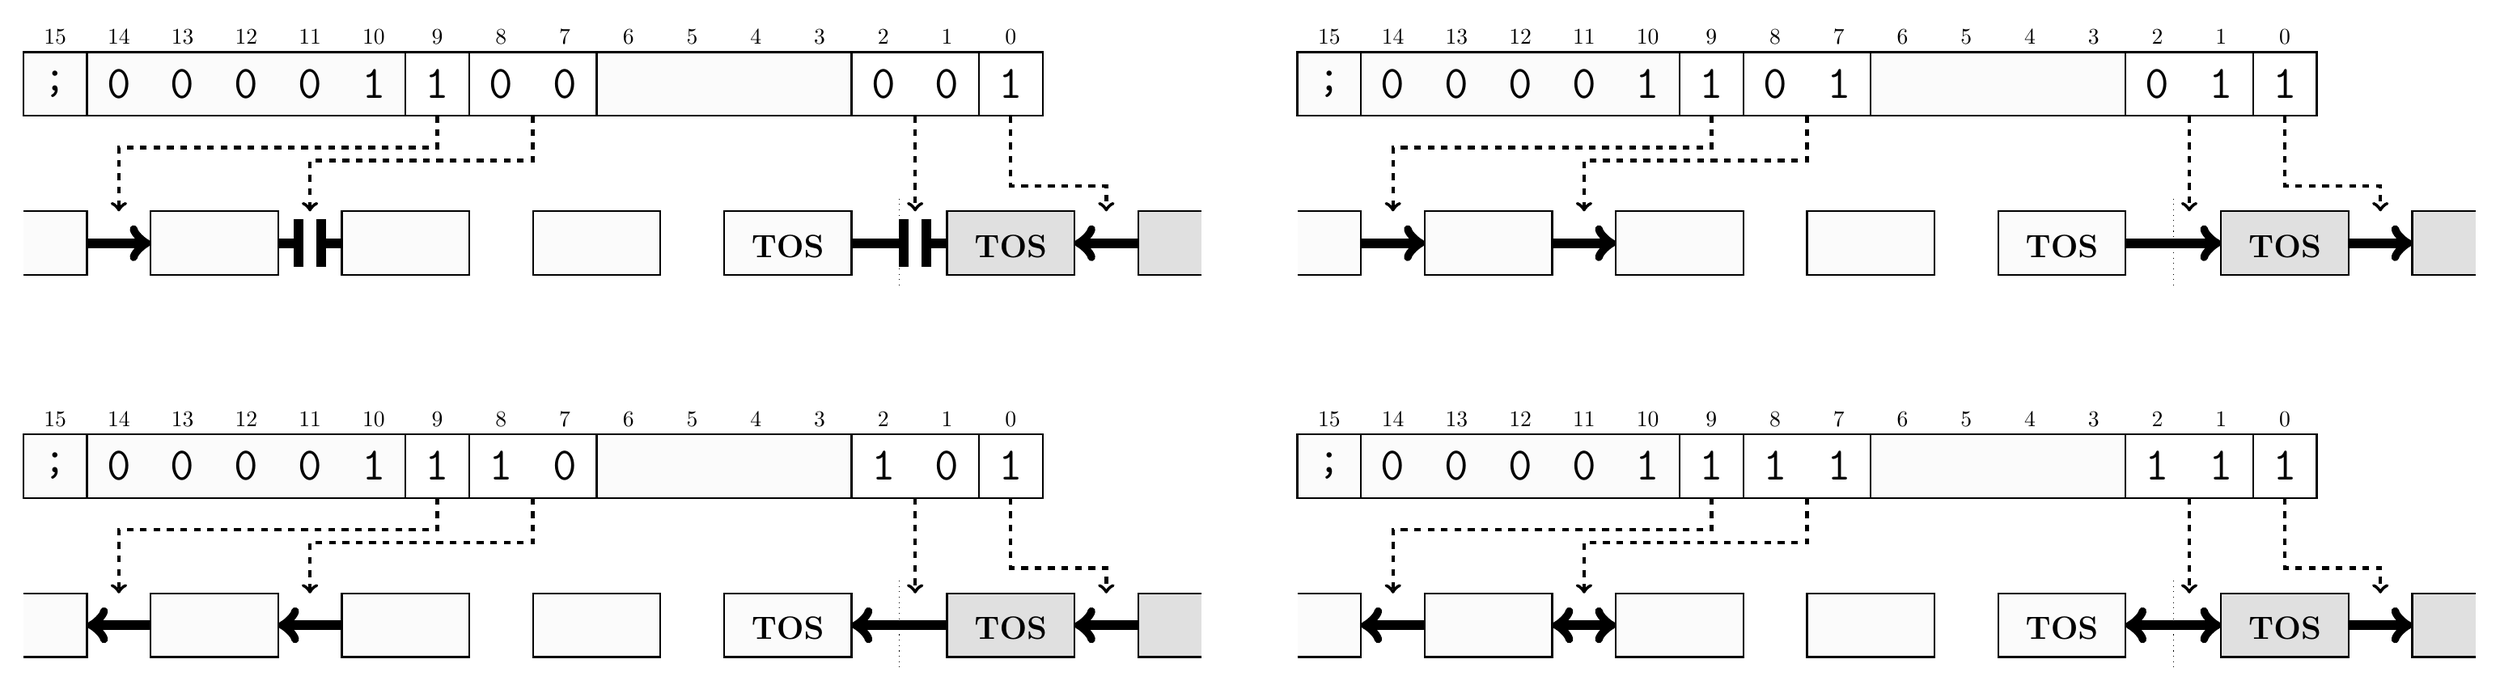
\begin{tikzpicture}
        %UST=00
         \begin{scope}[shift={(0,0)}]  
           %Stack instruction
           \draw [thick, fill=gray!3]  (1,3.5) rectangle (17,4.5);
           \draw [thick]               (1,3.5) rectangle  (2,4.5);
           \draw [thick]               (2,3.5) rectangle  (7,4.5); 
           \draw [thick, fill=white]   (7,3.5) rectangle  (8,4.5); 
           \draw [thick, fill=white]   (8,3.5) rectangle (10,4.5); 
           \draw [thick]               (10,3.5) rectangle (14,4.5); 
           %\draw [thick, fill=white]  (12,3.5) rectangle (14,4.5); 
           \draw [thick, fill=white]  (14,3.5) rectangle (16,4.5); 
           \draw [thick, fill=white]  (16,3.5) rectangle (17,4.5); 
           
           \node [above] at  (1.5,4.5) {15};
           \node [above] at  (2.5,4.5) {14};
           \node [above] at  (3.5,4.5) {13};
           \node [above] at  (4.5,4.5) {12};
           \node [above] at  (5.5,4.5) {11};
           \node [above] at  (6.5,4.5) {10};
           \node [above] at  (7.5,4.5) {9};
           \node [above] at  (8.5,4.5) {8};
           \node [above] at  (9.5,4.5) {7};
           \node [above] at (10.5,4.5) {6};
           \node [above] at (11.5,4.5) {5};
           \node [above] at (12.5,4.5) {4};
           \node [above] at (13.5,4.5) {3};
           \node [above] at (14.5,4.5) {2};
           \node [above] at (15.5,4.5) {1};
           \node [above] at (16.5,4.5) {0};
           
           \node         at (1.5,4)     {\huge{\texttt{;}}};
           \node         at (2.5,4)     {\huge{\texttt{0}}};
           \node         at (3.5,4)     {\huge{\texttt{0}}};
           \node         at (4.5,4)     {\huge{\texttt{0}}};
           \node         at (5.5,4)     {\huge{\texttt{0}}};   
           \node         at (6.5,4)     {\huge{\texttt{1}}};   
           
           \node         at (7.5,4)     {\huge{\texttt{1}}};   
           \node         at (8.5,4)     {\huge{\texttt{0}}};   
           \node         at (9.5,4)     {\huge{\texttt{0}}};   
           \node         at (14.5,4)    {\huge{\texttt{0}}};   
           \node         at (15.5,4)    {\huge{\texttt{0}}};   
           \node         at (16.5,4)    {\huge{\texttt{1}}};   
           
           %Bit field association
           \draw [ultra thick, dashed, ->]  (7.5,3.5)  -- (7.5,3)    -- (2.5,3)    -- (2.5,2);
           \draw [ultra thick, dashed, ->]  (9,3.5)    -- (9,2.8)    -- (5.5,2.8)  -- (5.5,2);
           \draw [ultra thick, dashed, ->]  (15,3.5)   -- (15,2);
           \draw [ultra thick, dashed, ->]  (16.5,3.5) -- (16.5,2.4) -- (18,2.4) -- (18,2);
           
           %Lower parameter stack
           \draw [thick, fill=gray!3]  (1,1) -- (2,1) -- (2,2) -- (1,2);
           \draw [line width=1ex, ->]  (2,1.5) --  (3,1.5);
           
           %Upper parameter stack
           \draw [thick, fill=gray!3]  (3,1) rectangle  (5,2);
           %\draw [line width=1ex, <->] (5,1.5) --  (6,1.5);
           \draw [line width=1ex, -|]     (5,1.5)  -- (5.4,1.5);
           \draw [line width=1ex, |-]     (5.6,1.5)   -- (6,1.5);
           
           \draw [thick, fill=gray!3]  (6,1) rectangle  (8,2);
           \draw [thick, fill=gray!3]  (9,1) rectangle  (11,2);
           \draw [thick, fill=gray!3]  (12,1) rectangle  (14,2);
           \node at (13,1.45)          {\Large{\textbf{TOS}}};        
                  
           %Stack boundary
           %\draw [line width=1ex, <->] (14,1.5)    --  (15.5,1.5);
           \draw [line width=1ex, -|]     (14,1.5) -- (14.9,1.5);
           \draw [line width=1ex, |-]   (15.1,1.5) -- (15.5,1.5);
           \draw [dotted]              (14.75,2.2) --  (14.75,0.8);
           
           %Upper return stack
           \draw [thick, fill=gray!24] (15.5,1) rectangle  (17.5,2);
           \node at (16.5,1.45)        {\Large{\textbf{TOS}}};
           \draw [line width=1ex, <-]  (17.5,1.5) --  (18.5,1.5);
           
           %Lower return stack
           \draw [thick, fill=gray!24] (19.5,1) -- (18.5,1) -- (18.5,2) -- (19.5,2);
         \end{scope}

         %UST=01
         \begin{scope}[shift={(20,0)}]
           %Stack instruction
           \draw [thick, fill=gray!3]  (1,3.5) rectangle (17,4.5);
           \draw [thick]               (1,3.5) rectangle  (2,4.5);
           \draw [thick]               (2,3.5) rectangle  (7,4.5); 
           \draw [thick, fill=white]   (7,3.5) rectangle  (8,4.5); 
           \draw [thick, fill=white]   (8,3.5) rectangle (10,4.5); 
           \draw [thick]               (10,3.5) rectangle (14,4.5); 
           %\draw [thick, fill=white]  (12,3.5) rectangle (14,4.5); 
           \draw [thick, fill=white]  (14,3.5) rectangle (16,4.5); 
           \draw [thick, fill=white]  (16,3.5) rectangle (17,4.5); 
           
           \node [above] at  (1.5,4.5) {15};
           \node [above] at  (2.5,4.5) {14};
           \node [above] at  (3.5,4.5) {13};
           \node [above] at  (4.5,4.5) {12};
           \node [above] at  (5.5,4.5) {11};
           \node [above] at  (6.5,4.5) {10};
           \node [above] at  (7.5,4.5) {9};
           \node [above] at  (8.5,4.5) {8};
           \node [above] at  (9.5,4.5) {7};
           \node [above] at (10.5,4.5) {6};
           \node [above] at (11.5,4.5) {5};
           \node [above] at (12.5,4.5) {4};
           \node [above] at (13.5,4.5) {3};
           \node [above] at (14.5,4.5) {2};
           \node [above] at (15.5,4.5) {1};
           \node [above] at (16.5,4.5) {0};
           
           \node         at (1.5,4)     {\huge{\texttt{;}}};
           \node         at (2.5,4)     {\huge{\texttt{0}}};
           \node         at (3.5,4)     {\huge{\texttt{0}}};
           \node         at (4.5,4)     {\huge{\texttt{0}}};
           \node         at (5.5,4)     {\huge{\texttt{0}}};   
           \node         at (6.5,4)     {\huge{\texttt{1}}};   
           
           \node         at (7.5,4)     {\huge{\texttt{1}}};   
           \node         at (8.5,4)     {\huge{\texttt{0}}};   
           \node         at (9.5,4)     {\huge{\texttt{1}}};   
           \node         at (14.5,4)    {\huge{\texttt{0}}};   
           \node         at (15.5,4)    {\huge{\texttt{1}}};   
           \node         at (16.5,4)    {\huge{\texttt{1}}};   
           
           %Bit field association
           \draw [ultra thick, dashed, ->]  (7.5,3.5)  -- (7.5,3)    -- (2.5,3)    -- (2.5,2);
           \draw [ultra thick, dashed, ->]  (9,3.5)    -- (9,2.8)    -- (5.5,2.8)  -- (5.5,2);
           \draw [ultra thick, dashed, ->]  (15,3.5)   -- (15,2);
           \draw [ultra thick, dashed, ->]  (16.5,3.5) -- (16.5,2.4) -- (18,2.4) -- (18,2);
           
           %Lower parameter stack
           \draw [thick, fill=gray!3]  (1,1) -- (2,1) -- (2,2) -- (1,2);
           \draw [line width=1ex, ->]  (2,1.5) --  (3,1.5);
           
           %Upper parameter stack
           \draw [thick, fill=gray!3]  (3,1) rectangle  (5,2);
           \draw [line width=1ex, ->] (5,1.5) --  (6,1.5);
           %\draw [line width=1ex, -|]     (5,1.5)  -- (5.4,1.5);
           %\draw [line width=1ex, |-]     (5.6,1.5)   -- (6,1.5);
           
           \draw [thick, fill=gray!3]  (6,1) rectangle  (8,2);
           \draw [thick, fill=gray!3]  (9,1) rectangle  (11,2);
           \draw [thick, fill=gray!3]  (12,1) rectangle  (14,2);
           \node at (13,1.45)          {\Large{\textbf{TOS}}};        
                  
           %Stack boundary
           \draw [line width=1ex, ->] (14,1.5)    --  (15.5,1.5);
           %\draw [line width=1ex, -|]     (14,1.5) -- (14.9,1.5);
           %\draw [line width=1ex, |-]   (15.1,1.5) -- (15.5,1.5);
           \draw [dotted]              (14.75,2.2) --  (14.75,0.8);
           
           %Upper return stack
           \draw [thick, fill=gray!24] (15.5,1) rectangle  (17.5,2);
           \node at (16.5,1.45)        {\Large{\textbf{TOS}}};
           \draw [line width=1ex, ->]  (17.5,1.5) --  (18.5,1.5);
           
           %Lower return stack
           \draw [thick, fill=gray!24] (19.5,1) -- (18.5,1) -- (18.5,2) -- (19.5,2);
         \end{scope}

         %UST=10
         \begin{scope}[shift={(0,-6)}]
           %Stack instruction
           \draw [thick, fill=gray!3]  (1,3.5) rectangle (17,4.5);
           \draw [thick]               (1,3.5) rectangle  (2,4.5);
           \draw [thick]               (2,3.5) rectangle  (7,4.5); 
           \draw [thick, fill=white]   (7,3.5) rectangle  (8,4.5); 
           \draw [thick, fill=white]   (8,3.5) rectangle (10,4.5); 
           \draw [thick]               (10,3.5) rectangle (14,4.5); 
           %\draw [thick, fill=white]  (12,3.5) rectangle (14,4.5); 
           \draw [thick, fill=white]  (14,3.5) rectangle (16,4.5); 
           \draw [thick, fill=white]  (16,3.5) rectangle (17,4.5); 
           
           \node [above] at  (1.5,4.5) {15};
           \node [above] at  (2.5,4.5) {14};
           \node [above] at  (3.5,4.5) {13};
           \node [above] at  (4.5,4.5) {12};
           \node [above] at  (5.5,4.5) {11};
           \node [above] at  (6.5,4.5) {10};
           \node [above] at  (7.5,4.5) {9};
           \node [above] at  (8.5,4.5) {8};
           \node [above] at  (9.5,4.5) {7};
           \node [above] at (10.5,4.5) {6};
           \node [above] at (11.5,4.5) {5};
           \node [above] at (12.5,4.5) {4};
           \node [above] at (13.5,4.5) {3};
           \node [above] at (14.5,4.5) {2};
           \node [above] at (15.5,4.5) {1};
           \node [above] at (16.5,4.5) {0};
           
           \node         at (1.5,4)     {\huge{\texttt{;}}};
           \node         at (2.5,4)     {\huge{\texttt{0}}};
           \node         at (3.5,4)     {\huge{\texttt{0}}};
           \node         at (4.5,4)     {\huge{\texttt{0}}};
           \node         at (5.5,4)     {\huge{\texttt{0}}};   
           \node         at (6.5,4)     {\huge{\texttt{1}}};   
           
           \node         at (7.5,4)     {\huge{\texttt{1}}};   
           \node         at (8.5,4)     {\huge{\texttt{1}}};   
           \node         at (9.5,4)     {\huge{\texttt{0}}};   
           \node         at (14.5,4)    {\huge{\texttt{1}}};   
           \node         at (15.5,4)    {\huge{\texttt{0}}};   
           \node         at (16.5,4)    {\huge{\texttt{1}}};   
           
           %Bit field association
           \draw [ultra thick, dashed, ->]  (7.5,3.5)  -- (7.5,3)    -- (2.5,3)    -- (2.5,2);
           \draw [ultra thick, dashed, ->]  (9,3.5)    -- (9,2.8)    -- (5.5,2.8)  -- (5.5,2);
           \draw [ultra thick, dashed, ->]  (15,3.5)   -- (15,2);
           \draw [ultra thick, dashed, ->]  (16.5,3.5) -- (16.5,2.4) -- (18,2.4) -- (18,2);
           
           %Lower parameter stack
           \draw [thick, fill=gray!3]  (1,1) -- (2,1) -- (2,2) -- (1,2);
           \draw [line width=1ex, <-]  (2,1.5) --  (3,1.5);
           
           %Upper parameter stack
           \draw [thick, fill=gray!3]  (3,1) rectangle  (5,2);
           \draw [line width=1ex, <-] (5,1.5) --  (6,1.5);
           %\draw [line width=1ex, -|]     (5,1.5)  -- (5.4,1.5);
           %\draw [line width=1ex, |-]     (5.6,1.5)   -- (6,1.5);
           
           \draw [thick, fill=gray!3]  (6,1) rectangle  (8,2);
           \draw [thick, fill=gray!3]  (9,1) rectangle  (11,2);
           \draw [thick, fill=gray!3]  (12,1) rectangle  (14,2);
           \node at (13,1.45)          {\Large{\textbf{TOS}}};        
                  
           %Stack boundary
           \draw [line width=1ex, <-] (14,1.5)    --  (15.5,1.5);
           %\draw [line width=1ex, -|]     (14,1.5) -- (14.9,1.5);
           %\draw [line width=1ex, |-]   (15.1,1.5) -- (15.5,1.5);
           \draw [dotted]              (14.75,2.2) --  (14.75,0.8);
           
           %Upper return stack
           \draw [thick, fill=gray!24] (15.5,1) rectangle  (17.5,2);
           \node at (16.5,1.45)        {\Large{\textbf{TOS}}};
           \draw [line width=1ex, <-]  (17.5,1.5) --  (18.5,1.5);
           
           %Lower return stack
           \draw [thick, fill=gray!24] (19.5,1) -- (18.5,1) -- (18.5,2) -- (19.5,2);
         \end{scope}

         %UST=11
         \begin{scope}[shift={(20,-6)}]
           %Stack instruction
           \draw [thick, fill=gray!3]  (1,3.5) rectangle (17,4.5);
           \draw [thick]               (1,3.5) rectangle  (2,4.5);
           \draw [thick]               (2,3.5) rectangle  (7,4.5); 
           \draw [thick, fill=white]   (7,3.5) rectangle  (8,4.5); 
           \draw [thick, fill=white]   (8,3.5) rectangle (10,4.5); 
           \draw [thick]               (10,3.5) rectangle (14,4.5); 
           %\draw [thick, fill=white]  (12,3.5) rectangle (14,4.5); 
           \draw [thick, fill=white]  (14,3.5) rectangle (16,4.5); 
           \draw [thick, fill=white]  (16,3.5) rectangle (17,4.5); 
           
           \node [above] at  (1.5,4.5) {15};
           \node [above] at  (2.5,4.5) {14};
           \node [above] at  (3.5,4.5) {13};
           \node [above] at  (4.5,4.5) {12};
           \node [above] at  (5.5,4.5) {11};
           \node [above] at  (6.5,4.5) {10};
           \node [above] at  (7.5,4.5) {9};
           \node [above] at  (8.5,4.5) {8};
           \node [above] at  (9.5,4.5) {7};
           \node [above] at (10.5,4.5) {6};
           \node [above] at (11.5,4.5) {5};
           \node [above] at (12.5,4.5) {4};
           \node [above] at (13.5,4.5) {3};
           \node [above] at (14.5,4.5) {2};
           \node [above] at (15.5,4.5) {1};
           \node [above] at (16.5,4.5) {0};
           
           \node         at (1.5,4)     {\huge{\texttt{;}}};
           \node         at (2.5,4)     {\huge{\texttt{0}}};
           \node         at (3.5,4)     {\huge{\texttt{0}}};
           \node         at (4.5,4)     {\huge{\texttt{0}}};
           \node         at (5.5,4)     {\huge{\texttt{0}}};   
           \node         at (6.5,4)     {\huge{\texttt{1}}};   
           
           \node         at (7.5,4)     {\huge{\texttt{1}}};   
           \node         at (8.5,4)     {\huge{\texttt{1}}};   
           \node         at (9.5,4)     {\huge{\texttt{1}}};   
           \node         at (14.5,4)    {\huge{\texttt{1}}};   
           \node         at (15.5,4)    {\huge{\texttt{1}}};   
           \node         at (16.5,4)    {\huge{\texttt{1}}};   
           
           %Bit field association
           \draw [ultra thick, dashed, ->]  (7.5,3.5)  -- (7.5,3)    -- (2.5,3)    -- (2.5,2);
           \draw [ultra thick, dashed, ->]  (9,3.5)    -- (9,2.8)    -- (5.5,2.8)  -- (5.5,2);
           \draw [ultra thick, dashed, ->]  (15,3.5)   -- (15,2);
           \draw [ultra thick, dashed, ->]  (16.5,3.5) -- (16.5,2.4) -- (18,2.4) -- (18,2);
           
           %Lower parameter stack
           \draw [thick, fill=gray!3]  (1,1) -- (2,1) -- (2,2) -- (1,2);
           \draw [line width=1ex, <-]  (2,1.5) --  (3,1.5);
           
           %Upper parameter stack
           \draw [thick, fill=gray!3]  (3,1) rectangle  (5,2);
           \draw [line width=1ex, <->] (5,1.5) --  (6,1.5);
           %\draw [line width=1ex, -|]     (5,1.5)  -- (5.4,1.5);
           %\draw [line width=1ex, |-]     (5.6,1.5)   -- (6,1.5);
           
           \draw [thick, fill=gray!3]  (6,1) rectangle  (8,2);
           \draw [thick, fill=gray!3]  (9,1) rectangle  (11,2);
           \draw [thick, fill=gray!3]  (12,1) rectangle  (14,2);
           \node at (13,1.45)          {\Large{\textbf{TOS}}};        
                  
           %Stack boundary
           \draw [line width=1ex, <->] (14,1.5)    --  (15.5,1.5);
           %\draw [line width=1ex, -|]     (14,1.5) -- (14.9,1.5);
           %\draw [line width=1ex, |-]   (15.1,1.5) -- (15.5,1.5);
           \draw [dotted]              (14.75,2.2) --  (14.75,0.8);
           
           %Upper return stack
           \draw [thick, fill=gray!24] (15.5,1) rectangle  (17.5,2);
           \node at (16.5,1.45)        {\Large{\textbf{TOS}}};
           \draw [line width=1ex, ->]  (17.5,1.5) --  (18.5,1.5);
           
           %Lower return stack
           \draw [thick, fill=gray!24] (19.5,1) -- (18.5,1) -- (18.5,2) -- (19.5,2);
         \end{scope}

      \end{tikzpicture}
    }
  }
  \caption{Transitions to and from the intermediate stack}
  \label{opcodes:stack:istrans}
  %\end{center}
\end{figure}
\end{samepage}



\subsubsection{Common Stack Operations}
\label{opcodes:stack:ops}
\tabref{opcodes:stack:mapping} shows how common \gls{stack} operations in \gls{forth} are mapped N1 instructions. 

\begingroup
\setlength{\LTleft}{-20cm plus -1fill}
\setlength{\LTright}{\LTleft}
\begin{center}
  \rowcolors{1}{gray!12}{white}                                         %set alternating row color
  \begin{longtable}{|c|c|c|c|}
    \rowcolor{white}
    \caption{Common stack operations}
    \label{opcodes:stack:mapping} \\
    %Header
    \hline                                     
    \rowcolor{gray!25}
    \multicolumn{1}{|c|}{\textbf{\rule{0pt}{2.5ex}Word}}       &  
    \multicolumn{1}{c|}{\textbf{\rule{0pt}{2.5ex}Description}} & 
    \multicolumn{1}{c|}{\textbf{\rule{0pt}{2.5ex}Transitions}} & 
    \multicolumn{1}{c|}{\textbf{\rule{0pt}{2.5ex}Opcode}} \\
    \hline
    \endhead                               
    %Footers
    \hline
    \rowcolor{white}
    \multicolumn{4}{r}{\tiny{...continued}} \\
    \endfoot
    \hline
    \endlastfoot

    %DROP
    \texttt{DROP} &
    ( x -- ) &
    \multicolumn{1}{m{21.35em}|}{
    \scalebox{0.4} {
      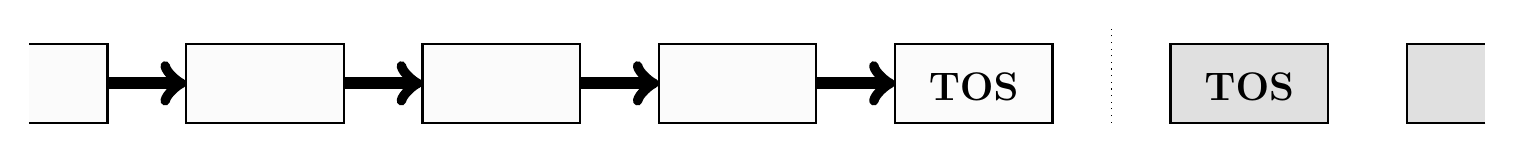
\begin{tikzpicture}
        \draw [thick, fill=gray!3]  (0,0) -- (1,0) -- (1,1) -- (0,1);%
        \draw [line width=1ex, ->]  (1,0.5) -- (2,0.5);              %
        \draw [thick, fill=gray!3]  (2,0) rectangle (4,1);           %PS+3
        \draw [line width=1ex, ->]  (4,0.5) -- (5,0.5);              %
        \draw [thick, fill=gray!3]  (5,0) rectangle (7,1);           %PS+2
        \draw [line width=1ex, ->]  (7,0.5) -- (8,0.5);              %
        \draw [thick, fill=gray!3]  (8,0) rectangle (10,1);          %PS+1
        \draw [line width=1ex, ->]  (10,0.5) -- (11,0.5);            %
        \draw [thick, fill=gray!3]  (11,0) rectangle (13,1);         %PS TOS
        \node at (12,0.45)          {\Large{\textbf{TOS}}};          %
        %\draw [line width=1ex, --] (13,0.5)  -- (14.5,0.5);         %
        \draw [dotted]              (13.75,0) -- (13.75,1.2);        %
        \draw [thick, fill=gray!24] (14.5,0) rectangle (16.5,1);     %RS TOS
        \node at (15.5,0.45)        {\Large{\textbf{TOS}}};          %
        %\draw [line width=1ex, --] (16.5,0.5) -- (17.5,0.5);        % 
        \draw [thick, fill=gray!24] (18.5,0) -- (17.5,0) -- (17.5,1) -- (18.5,1);
       \end{tikzpicture}
    }} &
    \texttt{0x06A8} \\ \hline   

    %DUP
    \texttt{DUP} &
    ( x -- x x ) &
    \multicolumn{1}{m{21.35em}|}{
    \scalebox{0.4} {
      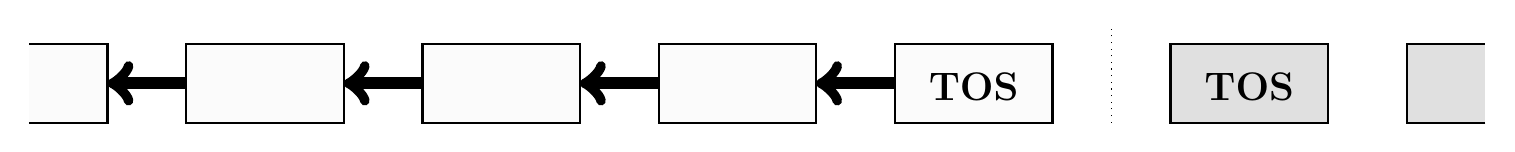
\begin{tikzpicture}
        \draw [thick, fill=gray!3]  (0,0) -- (1,0) -- (1,1) -- (0,1);%
        \draw [line width=1ex, <-]  (1,0.5) -- (2,0.5);              %
        \draw [thick, fill=gray!3]  (2,0) rectangle (4,1);           %PS+3
        \draw [line width=1ex, <-]  (4,0.5) -- (5,0.5);              %
        \draw [thick, fill=gray!3]  (5,0) rectangle (7,1);           %PS+2
        \draw [line width=1ex, <-]  (7,0.5) -- (8,0.5);              %
        \draw [thick, fill=gray!3]  (8,0) rectangle (10,1);          %PS+1
        \draw [line width=1ex, <-]  (10,0.5) -- (11,0.5);            %
        \draw [thick, fill=gray!3]  (11,0) rectangle (13,1);         %PS TOS
        \node at (12,0.45)          {\Large{\textbf{TOS}}};          %
        %\draw [line width=1ex, --] (13,0.5)  -- (14.5,0.5);         %
        \draw [dotted]              (13.75,0) -- (13.75,1.2);        %
        \draw [thick, fill=gray!24] (14.5,0) rectangle (16.5,1);     %RS TOS
        \node at (15.5,0.45)        {\Large{\textbf{TOS}}};          %
        %\draw [line width=1ex, --] (16.5,0.5) -- (17.5,0.5);        % 
        \draw [thick, fill=gray!24] (18.5,0) -- (17.5,0) -- (17.5,1) -- (18.5,1);
       \end{tikzpicture}
    }} &
    \texttt{0x0750} \\ \hline  

    %SWAP
    \texttt{SWAP} &
    ( x1 x2 -- x2 x1 ) &
    \multicolumn{1}{m{21.35em}|}{
    \scalebox{0.4} {
      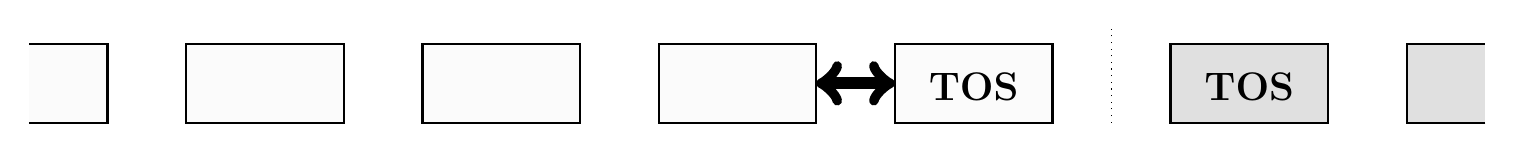
\begin{tikzpicture}
        \draw [thick, fill=gray!3]  (0,0) -- (1,0) -- (1,1) -- (0,1);%
        %\draw [line width=1ex, --] (1,0.5) -- (2,0.5);              %
        \draw [thick, fill=gray!3]  (2,0) rectangle (4,1);           %PS+3
        %\draw [line width=1ex, --] (4,0.5) -- (5,0.5);              %
        \draw [thick, fill=gray!3]  (5,0) rectangle (7,1);           %PS+2
        %\draw [line width=1ex, --] (7,0.5) -- (8,0.5);              %
        \draw [thick, fill=gray!3]  (8,0) rectangle (10,1);          %PS+1
        \draw [line width=1ex, <->] (10,0.5) -- (11,0.5);            %
        \draw [thick, fill=gray!3]  (11,0) rectangle (13,1);         %PS TOS
        \node at (12,0.45)          {\Large{\textbf{TOS}}};          %
        %\draw [line width=1ex, --] (13,0.5)  -- (14.5,0.5);         %
        \draw [dotted]              (13.75,0) -- (13.75,1.2);        %
        \draw [thick, fill=gray!24] (14.5,0) rectangle (16.5,1);     %RS TOS
        \node at (15.5,0.45)        {\Large{\textbf{TOS}}};          %
        %\draw [line width=1ex, --] (16.5,0.5) -- (17.5,0.5);        % 
        \draw [thick, fill=gray!24] (18.5,0) -- (17.5,0) -- (17.5,1) -- (18.5,1);
       \end{tikzpicture}
    }} &
    \texttt{0x0418} \\ \hline     

    %OVER
    \texttt{OVER} &
    ( x1 x2 -- x1 x2 x1 ) &
    \multicolumn{1}{m{21.35em}|}{
    \scalebox{0.4} {
      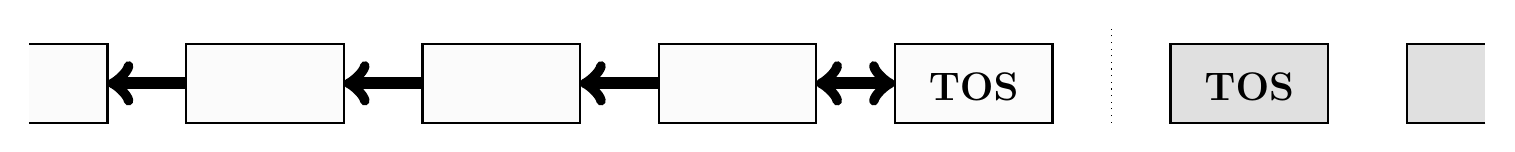
\begin{tikzpicture}
        \draw [thick, fill=gray!3]  (0,0) -- (1,0) -- (1,1) -- (0,1);%
        \draw [line width=1ex, <-]  (1,0.5) -- (2,0.5);              %
        \draw [thick, fill=gray!3]  (2,0) rectangle (4,1);           %PS+3
        \draw [line width=1ex, <-]  (4,0.5) -- (5,0.5);              %
        \draw [thick, fill=gray!3]  (5,0) rectangle (7,1);           %PS+2
        \draw [line width=1ex, <-]  (7,0.5) -- (8,0.5);              %
        \draw [thick, fill=gray!3]  (8,0) rectangle (10,1);          %PS+1
        \draw [line width=1ex, <->] (10,0.5) -- (11,0.5);            %
        \draw [thick, fill=gray!3]  (11,0) rectangle (13,1);         %PS TOS
        \node at (12,0.45)          {\Large{\textbf{TOS}}};          %
        %\draw [line width=1ex, --] (13,0.5)  -- (14.5,0.5);         %
        \draw [dotted]              (13.75,0) -- (13.75,1.2);        %
        \draw [thick, fill=gray!24] (14.5,0) rectangle (16.5,1);     %RS TOS
        \node at (15.5,0.45)        {\Large{\textbf{TOS}}};          %
        %\draw [line width=1ex, --] (16.5,0.5) -- (17.5,0.5);        % 
        \draw [thick, fill=gray!24] (18.5,0) -- (17.5,0) -- (17.5,1) -- (18.5,1);
       \end{tikzpicture}
    }} &
    \texttt{0x0758} \\ \hline     

    %NIP
    \texttt{NIP} &
    ( x1 x2 -- x2 ) &
    \multicolumn{1}{m{21.35em}|}{
    \scalebox{0.4} {
      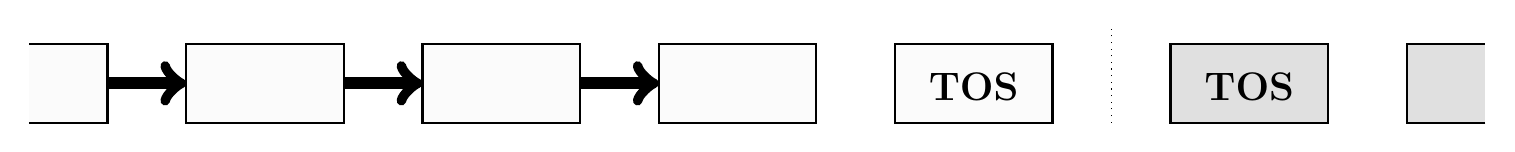
\begin{tikzpicture}
        \draw [thick, fill=gray!3]  (0,0) -- (1,0) -- (1,1) -- (0,1);%
        \draw [line width=1ex, ->]  (1,0.5) -- (2,0.5);              %
        \draw [thick, fill=gray!3]  (2,0) rectangle (4,1);           %PS+3
        \draw [line width=1ex, ->]  (4,0.5) -- (5,0.5);              %
        \draw [thick, fill=gray!3]  (5,0) rectangle (7,1);           %PS+2
        \draw [line width=1ex, ->]  (7,0.5) -- (8,0.5);              %
        \draw [thick, fill=gray!3]  (8,0) rectangle (10,1);          %PS+1
        %\draw [line width=1ex, ->] (10,0.5) -- (11,0.5);            %
        \draw [thick, fill=gray!3]  (11,0) rectangle (13,1);         %PS TOS
        \node at (12,0.45)          {\Large{\textbf{TOS}}};          %
        %\draw [line width=1ex, --] (13,0.5)  -- (14.5,0.5);         %
        \draw [dotted]              (13.75,0) -- (13.75,1.2);        %
        \draw [thick, fill=gray!24] (14.5,0) rectangle (16.5,1);     %RS TOS
        \node at (15.5,0.45)        {\Large{\textbf{TOS}}};          %
        %\draw [line width=1ex, --] (16.5,0.5) -- (17.5,0.5);        % 
        \draw [thick, fill=gray!24] (18.5,0) -- (17.5,0) -- (17.5,1) -- (18.5,1);
       \end{tikzpicture}
    }} &
    \texttt{0x06A0} \\ \hline  

    %TUCK
    \texttt{TUCK} &
    ( x1 x2 -- x2 x1 x2 ) &
    \multicolumn{1}{m{21.35em}|}{
    \scalebox{0.4} {
      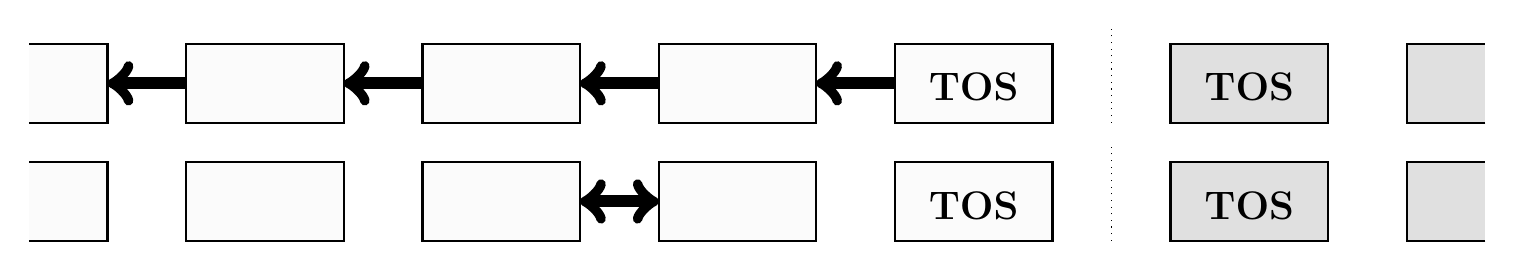
\begin{tikzpicture}
        \draw [thick, fill=gray!3]  (0,1.5) -- (1,1.5) -- (1,2.5) -- (0,2.5);%
        \draw [line width=1ex, <-]  (1,2)   -- (2,2);                %
        \draw [thick, fill=gray!3]  (2,1.5) rectangle (4,2.5);       %PS+3
        \draw [line width=1ex, <-]  (4,2)   -- (5,2);                %
        \draw [thick, fill=gray!3]  (5,1.5) rectangle (7,2.5);       %PS+2
        \draw [line width=1ex, <-]  (7,2)   -- (8,2);                %
        \draw [thick, fill=gray!3]  (8,1.5) rectangle (10,2.5);      %PS+1
        \draw [line width=1ex, <-]  (10,2)  -- (11,2);               %
        \draw [thick, fill=gray!3]  (11,1.5) rectangle (13,2.5);     %PS TOS
        \node at (12,1.95)          {\Large{\textbf{TOS}}};          %
        %\draw [line width=1ex, --] (13,2)  -- (14.5,2);             %
        \draw [dotted]              (13.75,1.5) -- (13.75,2.7);      %
        \draw [thick, fill=gray!24] (14.5,1.5) rectangle (16.5,2.5); %RS TOS
        \node at (15.5,1.95)        {\Large{\textbf{TOS}}};          %
        %\draw [line width=1ex, --] (16.5,2) -- (17.5,2);            % 
        \draw [thick, fill=gray!24] (18.5,1.5) -- (17.5,1.5) -- (17.5,2.5) -- (18.5,2.5);

        \draw [thick, fill=gray!3]  (0,0) -- (1,0) -- (1,1) -- (0,1);%
        %\draw [line width=1ex, --] (1,0.5) -- (2,0.5);              %
        \draw [thick, fill=gray!3]  (2,0) rectangle (4,1);           %PS+3
        %\draw [line width=1ex, --] (4,0.5) -- (5,0.5);              %
        \draw [thick, fill=gray!3]  (5,0) rectangle (7,1);           %PS+2
        \draw [line width=1ex, <->] (7,0.5) -- (8,0.5);              %
        \draw [thick, fill=gray!3]  (8,0) rectangle (10,1);          %PS+1
        %\draw [line width=1ex, --] (10,0.5) -- (11,0.5);            %
        \draw [thick, fill=gray!3]  (11,0) rectangle (13,1);         %PS TOS
        \node at (12,0.45)          {\Large{\textbf{TOS}}};          %
        %\draw [line width=1ex, --] (13,0.5)  -- (14.5,0.5);         %
        \draw [dotted]              (13.75,0) -- (13.75,1.2);        %
        \draw [thick, fill=gray!24] (14.5,0) rectangle (16.5,1);     %RS TOS
        \node at (15.5,0.45)        {\Large{\textbf{TOS}}};          %
        %\draw [line width=1ex, --] (16.5,0.5) -- (17.5,0.5);        % 
        \draw [thick, fill=gray!24] (18.5,0) -- (17.5,0) -- (17.5,1) -- (18.5,1);
       \end{tikzpicture}
    }} &
    \multicolumn{1}{m{4.25em}|}{
    \makecell[c]{ 
      \texttt{0x0750} \\ 
      \texttt{0x0460}
    }} \\ \hline

    %ROT
    \texttt{ROT} &
    ( x1 x2 x3 -- x2 x3 x1 ) &
    \multicolumn{1}{m{21.35em}|}{
    \scalebox{0.4} {
      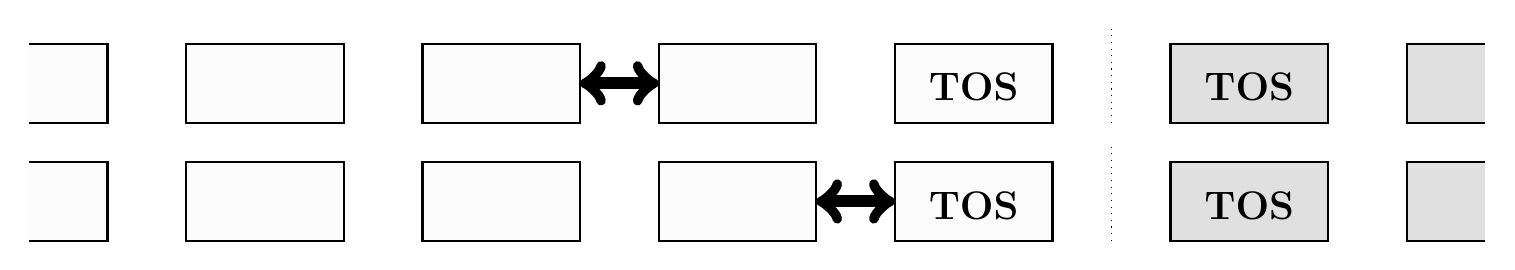
\begin{tikzpicture}
        \draw [thick, fill=gray!3]  (0,1.5) -- (1,1.5) -- (1,2.5) -- (0,2.5);%
        %\draw [line width=1ex, --] (1,2)   -- (2,2);                %
        \draw [thick, fill=gray!3]  (2,1.5) rectangle (4,2.5);       %PS+3
        %\draw [line width=1ex, --] (4,2)   -- (5,2);                %
        \draw [thick, fill=gray!3]  (5,1.5) rectangle (7,2.5);       %PS+2
        \draw [line width=1ex, <->] (7,2)   -- (8,2);                %
        \draw [thick, fill=gray!3]  (8,1.5) rectangle (10,2.5);      %PS+1
        %\draw [line width=1ex, --] (10,2) -- (11,2);                %
        \draw [thick, fill=gray!3]  (11,1.5) rectangle (13,2.5);     %PS TOS
        \node at (12,1.95)          {\Large{\textbf{TOS}}};          %
        %\draw [line width=1ex, --] (13,2)  -- (14.5,2);             %
        \draw [dotted]              (13.75,1.5) -- (13.75,2.7);      %
        \draw [thick, fill=gray!24] (14.5,1.5) rectangle (16.5,2.5); %RS TOS
        \node at (15.5,1.95)        {\Large{\textbf{TOS}}};          %
        %\draw [line width=1ex, --] (16.5,2) -- (17.5,2);            % 
        \draw [thick, fill=gray!24] (18.5,1.5) -- (17.5,1.5) -- (17.5,2.5) -- (18.5,2.5);

        \draw [thick, fill=gray!3]  (0,0) -- (1,0) -- (1,1) -- (0,1);%
        %\draw [line width=1ex, --] (1,0.5) -- (2,0.5);              %
        \draw [thick, fill=gray!3]  (2,0) rectangle (4,1);           %PS+3
        %\draw [line width=1ex, --] (4,0.5) -- (5,0.5);              %
        \draw [thick, fill=gray!3]  (5,0) rectangle (7,1);           %PS+2
        %\draw [line width=1ex, --] (7,0.5) -- (8,0.5);              %
        \draw [thick, fill=gray!3]  (8,0) rectangle (10,1);          %PS+1
        \draw [line width=1ex, <->] (10,0.5) -- (11,0.5);            %
        \draw [thick, fill=gray!3]  (11,0) rectangle (13,1);         %PS TOS
        \node at (12,0.45)          {\Large{\textbf{TOS}}};          %
        %\draw [line width=1ex, --] (13,0.5)  -- (14.5,0.5);         %
        \draw [dotted]              (13.75,0) -- (13.75,1.2);        %
        \draw [thick, fill=gray!24] (14.5,0) rectangle (16.5,1);     %RS TOS
        \node at (15.5,0.45)        {\Large{\textbf{TOS}}};          %
        %\draw [line width=1ex, --] (16.5,0.5) -- (17.5,0.5);        % 
        \draw [thick, fill=gray!24] (18.5,0) -- (17.5,0) -- (17.5,1) -- (18.5,1);
       \end{tikzpicture}
    }} &
    \multicolumn{1}{m{4.25em}|}{
    \makecell[c]{ 
      \texttt{0x0460} \\ 
      \texttt{0x0418}
    }} \\ \hline
    
    %-ROT
    \texttt{-ROT} &
    ( x1 x2 x3 -- x3 x1 x2 ) &
    \multicolumn{1}{m{21.35em}|}{
    \scalebox{0.4} {
      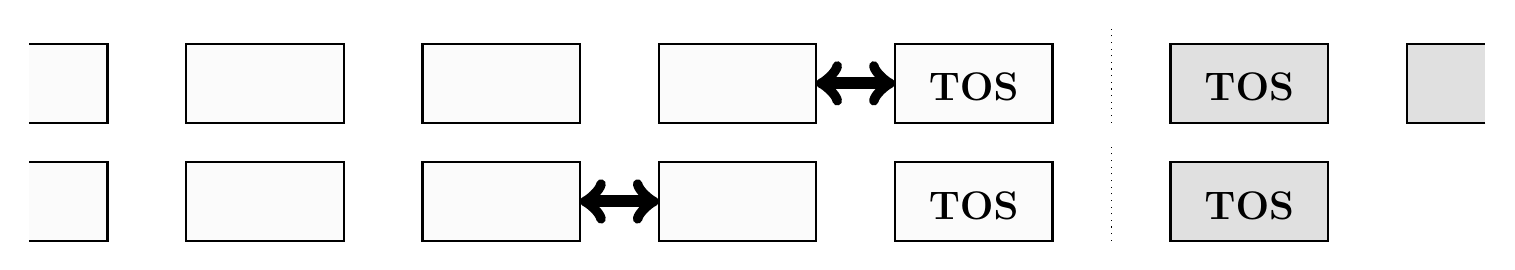
\begin{tikzpicture}
        \draw [thick, fill=gray!3]  (0,1.5) -- (1,1.5) -- (1,2.5) -- (0,2.5);%
        %\draw [line width=1ex, --] (1,2)   -- (2,2);                %
        \draw [thick, fill=gray!3]  (2,1.5) rectangle (4,2.5);       %PS+3
        %\draw [line width=1ex, --] (4,2)   -- (5,2);                %
        \draw [thick, fill=gray!3]  (5,1.5) rectangle (7,2.5);       %PS+2
        %\draw [line width=1ex, --] (7,2)   -- (8,2);                %
        \draw [thick, fill=gray!3]  (8,1.5) rectangle (10,2.5);      %PS+1
        \draw [line width=1ex, <->] (10,2) -- (11,2);                %
        \draw [thick, fill=gray!3]  (11,1.5) rectangle (13,2.5);     %PS TOS
        \node at (12,1.95)          {\Large{\textbf{TOS}}};          %
        %\draw [line width=1ex, --] (13,2)  -- (14.5,2);             %
        \draw [dotted]              (13.75,1.5) -- (13.75,2.7);      %
        \draw [thick, fill=gray!24] (14.5,1.5) rectangle (16.5,2.5); %RS TOS
        \node at (15.5,1.95)        {\Large{\textbf{TOS}}};          %
        %\draw [line width=1ex, --] (16.5,2) -- (17.5,2);            % 
        \draw [thick, fill=gray!24] (18.5,1.5) -- (17.5,1.5) -- (17.5,2.5) -- (18.5,2.5);

        \draw [thick, fill=gray!3]  (0,0) -- (1,0) -- (1,1) -- (0,1);%
        %\draw [line width=1ex, --] (1,0.5) -- (2,0.5);              %
        \draw [thick, fill=gray!3]  (2,0) rectangle (4,1);           %PS+3
        %\draw [line width=1ex, --] (4,0.5) -- (5,0.5);              %
        \draw [thick, fill=gray!3]  (5,0) rectangle (7,1);           %PS+2
        \draw [line width=1ex, <->] (7,0.5) -- (8,0.5);              %
        \draw [thick, fill=gray!3]  (8,0) rectangle (10,1);          %PS+1
        %\draw [line width=1ex, --] (10,0.5) -- (11,0.5);            %
        \draw [thick, fill=gray!3]  (11,0) rectangle (13,1);         %PS TOS
        \node at (12,0.45)          {\Large{\textbf{TOS}}};          %
        %\draw [line width=1ex, --] (13,0.5)  -- (14.5,0.5);         %
        \draw [dotted]              (13.75,0) -- (13.75,1.2);        %
        \draw [thick, fill=gray!24] (14.5,0) rectangle (16.5,1);     %RS TOS
        \node at (15.5,0.45)        {\Large{\textbf{TOS}}};          %
        %\draw [line width=1ex, --] (16.5,0.5) -- (17.5,0.5);        % 
      \end{tikzpicture}
    }} &
    \multicolumn{1}{m{4.25em}|}{
    \makecell[c]{ 
      \texttt{0x0418} \\ 
      \texttt{0x0460}
    }} \\ \hline

    %RDROP
    \texttt{RDROP} &
    ( R: x -- ) &
    \multicolumn{1}{m{21.35em}|}{
    \scalebox{0.4} {
      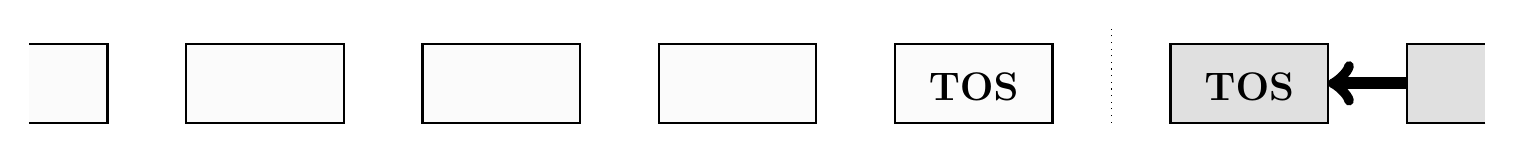
\begin{tikzpicture}
        \draw [thick, fill=gray!3]  (0,0) -- (1,0) -- (1,1) -- (0,1);%
        %\draw [line width=1ex, --] (1,0.5) -- (2,0.5);              %
        \draw [thick, fill=gray!3]  (2,0) rectangle (4,1);           %PS+3
        %\draw [line width=1ex, --] (4,0.5) -- (5,0.5);              %
        \draw [thick, fill=gray!3]  (5,0) rectangle (7,1);           %PS+2
        %\draw [line width=1ex, --] (7,0.5) -- (8,0.5);              %
        \draw [thick, fill=gray!3]  (8,0) rectangle (10,1);          %PS+1
        %\draw [line width=1ex, --] (10,0.5) -- (11,0.5);            %
        \draw [thick, fill=gray!3]  (11,0) rectangle (13,1);         %PS TOS
        \node at (12,0.45)          {\Large{\textbf{TOS}}};          %
        %\draw [line width=1ex, --] (13,0.5)  -- (14.5,0.5);         %
        \draw [dotted]              (13.75,0) -- (13.75,1.2);        %
        \draw [thick, fill=gray!24] (14.5,0) rectangle (16.5,1);     %RS TOS
        \node at (15.5,0.45)        {\Large{\textbf{TOS}}};          %
        \draw [line width=1ex, <-]  (16.5,0.5) -- (17.5,0.5);        % 
        \draw [thick, fill=gray!24] (18.5,0) -- (17.5,0) -- (17.5,1) -- (18.5,1);
       \end{tikzpicture}
    }} &
    \texttt{0x0401} \\ \hline     

    %RDUP
    \texttt{RDUP} &
    ( R: x -- x x ) &
    \multicolumn{1}{m{21.35em}|}{
    \scalebox{0.4} {
      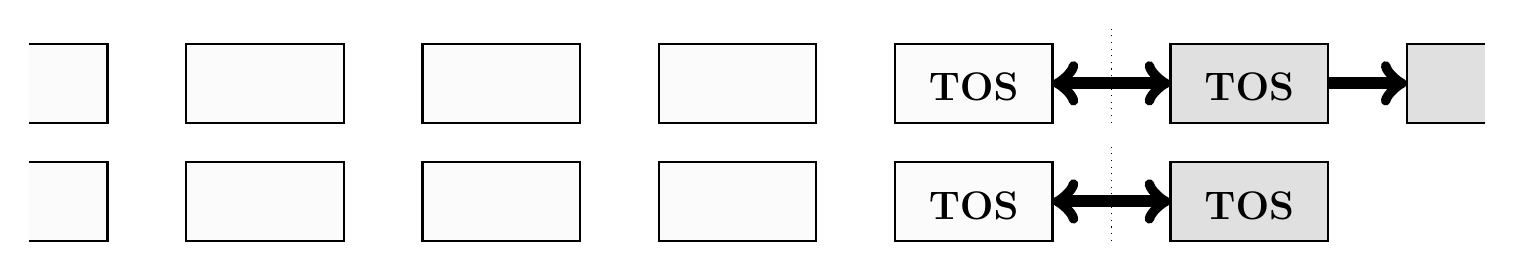
\begin{tikzpicture}
        \draw [thick, fill=gray!3]  (0,1.5) -- (1,1.5) -- (1,2.5) -- (0,2.5);%
        %\draw [line width=1ex, --] (1,2)   -- (2,2);                %
        \draw [thick, fill=gray!3]  (2,1.5) rectangle (4,2.5);       %PS+3
        %\draw [line width=1ex, --] (4,2)   -- (5,2);                %
        \draw [thick, fill=gray!3]  (5,1.5) rectangle (7,2.5);       %PS+2
        %\draw [line width=1ex, --] (7,2)   -- (8,2);                %
        \draw [thick, fill=gray!3]  (8,1.5) rectangle (10,2.5);      %PS+1
        %\draw [line width=1ex, --] (10,2) -- (11,2);                %
        \draw [thick, fill=gray!3]  (11,1.5) rectangle (13,2.5);     %PS TOS
        \node at (12,1.95)          {\Large{\textbf{TOS}}};          %
        \draw [line width=1ex, <->] (13,2)  -- (14.5,2);             %
        \draw [dotted]              (13.75,1.5) -- (13.75,2.7);      %
        \draw [thick, fill=gray!24] (14.5,1.5) rectangle (16.5,2.5); %RS TOS
        \node at (15.5,1.95)        {\Large{\textbf{TOS}}};          %
        \draw [line width=1ex, ->]  (16.5,2) -- (17.5,2);            % 
        \draw [thick, fill=gray!24] (18.5,1.5) -- (17.5,1.5) -- (17.5,2.5) -- (18.5,2.5);

        \draw [thick, fill=gray!3]  (0,0) -- (1,0) -- (1,1) -- (0,1);%
        %\draw [line width=1ex, --] (1,0.5) -- (2,0.5);              %
        \draw [thick, fill=gray!3]  (2,0) rectangle (4,1);           %PS+3
        %\draw [line width=1ex, --] (4,0.5) -- (5,0.5);              %
        \draw [thick, fill=gray!3]  (5,0) rectangle (7,1);           %PS+2
        %\draw [line width=1ex, --] (7,0.5) -- (8,0.5);              %
        \draw [thick, fill=gray!3]  (8,0) rectangle (10,1);          %PS+1
        %\draw [line width=1ex, --] (10,0.5) -- (11,0.5);            %
        \draw [thick, fill=gray!3]  (11,0) rectangle (13,1);         %PS TOS
        \node at (12,0.45)          {\Large{\textbf{TOS}}};          %
        \draw [line width=1ex, <->] (13,0.5)  -- (14.5,0.5);         %
        \draw [dotted]              (13.75,0) -- (13.75,1.2);        %
        \draw [thick, fill=gray!24] (14.5,0) rectangle (16.5,1);     %RS TOS
        \node at (15.5,0.45)        {\Large{\textbf{TOS}}};          %
        %\draw [line width=1ex, --] (16.5,0.5) -- (17.5,0.5);        % 
      \end{tikzpicture}
    }} &
    \multicolumn{1}{m{4.25em}|}{
    \makecell[c]{ 
      \texttt{0x0407} \\ 
      \texttt{0x0406}
    }} \\ \hline

    %>R
    \texttt{>R} &
    \multicolumn{1}{m{18.3em}|}{
    \makecell[c]{ 
      ( x -- )\\
      ( R: -- x )
    }} &
    \multicolumn{1}{m{21.35em}|}{
    \scalebox{0.4} {
      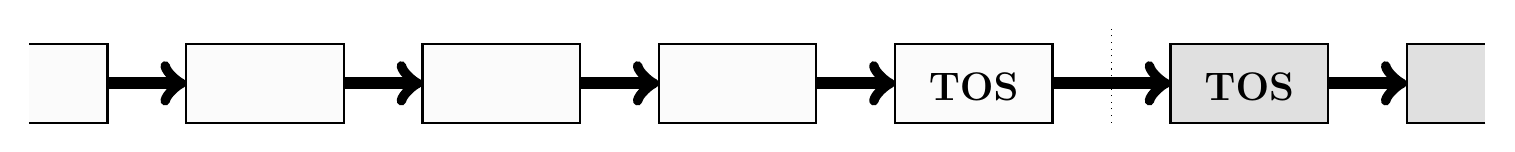
\begin{tikzpicture}
        \draw [thick, fill=gray!3]  (0,0) -- (1,0) -- (1,1) -- (0,1);%
        \draw [line width=1ex, ->]  (1,0.5) -- (2,0.5);              %
        \draw [thick, fill=gray!3]  (2,0) rectangle (4,1);           %PS+3
        \draw [line width=1ex, ->]  (4,0.5) -- (5,0.5);              %
        \draw [thick, fill=gray!3]  (5,0) rectangle (7,1);           %PS+2
        \draw [line width=1ex, ->]  (7,0.5) -- (8,0.5);              %
        \draw [thick, fill=gray!3]  (8,0) rectangle (10,1);          %PS+1
        \draw [line width=1ex, ->]  (10,0.5) -- (11,0.5);            %
        \draw [thick, fill=gray!3]  (11,0) rectangle (13,1);         %PS TOS
        \node at (12,0.45)          {\Large{\textbf{TOS}}};          %
        \draw [line width=1ex, ->]  (13,0.5)  -- (14.5,0.5);         %
        \draw [dotted]              (13.75,0) -- (13.75,1.2);        %
        \draw [thick, fill=gray!24] (14.5,0) rectangle (16.5,1);     %RS TOS
        \node at (15.5,0.45)        {\Large{\textbf{TOS}}};          %
        \draw [line width=1ex, ->]  (16.5,0.5) -- (17.5,0.5);        % 
        \draw [thick, fill=gray!24] (18.5,0) -- (17.5,0) -- (17.5,1) -- (18.5,1);
       \end{tikzpicture}
    }} &
    \texttt{0x06AB} \\ \hline  

    %R@
    \texttt{R@} &
    \multicolumn{1}{m{18.3em}|}{
    \makecell[c]{ 
      ( -- x )\\
      ( R: x -- x )
    }} &
    \multicolumn{1}{m{21.35em}|}{
    \scalebox{0.4} {
      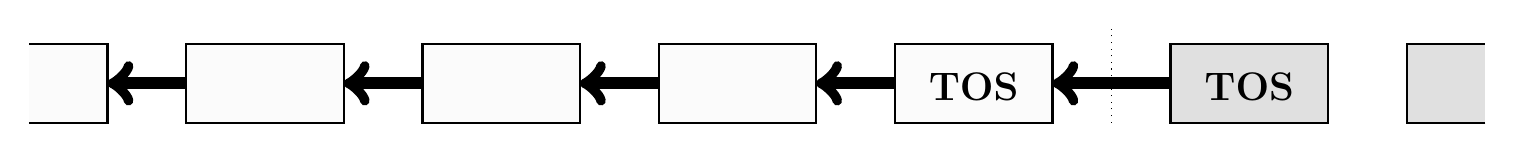
\begin{tikzpicture}
        \draw [thick, fill=gray!3]  (0,0) -- (1,0) -- (1,1) -- (0,1);%
        \draw [line width=1ex, <-]  (1,0.5) -- (2,0.5);              %
        \draw [thick, fill=gray!3]  (2,0) rectangle (4,1);           %PS+3
        \draw [line width=1ex, <-]  (4,0.5) -- (5,0.5);              %
        \draw [thick, fill=gray!3]  (5,0) rectangle (7,1);           %PS+2
        \draw [line width=1ex, <-]  (7,0.5) -- (8,0.5);              %
        \draw [thick, fill=gray!3]  (8,0) rectangle (10,1);          %PS+1
        \draw [line width=1ex, <-]  (10,0.5) -- (11,0.5);            %
        \draw [thick, fill=gray!3]  (11,0) rectangle (13,1);         %PS TOS
        \node at (12,0.45)          {\Large{\textbf{TOS}}};          %
        \draw [line width=1ex, <-]  (13,0.5)  -- (14.5,0.5);         %
        \draw [dotted]              (13.75,0) -- (13.75,1.2);        %
        \draw [thick, fill=gray!24] (14.5,0) rectangle (16.5,1);     %RS TOS
        \node at (15.5,0.45)        {\Large{\textbf{TOS}}};          %
        %\draw [line width=1ex, --] (16.5,0.5) -- (17.5,0.5);        % 
        \draw [thick, fill=gray!24] (18.5,0) -- (17.5,0) -- (17.5,1) -- (18.5,1);
       \end{tikzpicture}
    }} &
    \texttt{0x0754} \\ \hline  

    %R>
    \texttt{R>} &
    \multicolumn{1}{m{18.3em}|}{
    \makecell[c]{ 
      ( -- x )\\
      ( R: x -- )
    }} &
    \multicolumn{1}{m{21.35em}|}{
    \scalebox{0.4} {
      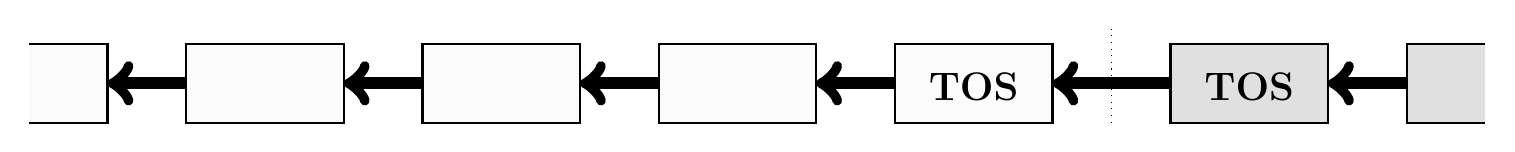
\begin{tikzpicture}
        \draw [thick, fill=gray!3]  (0,0) -- (1,0) -- (1,1) -- (0,1);%
        \draw [line width=1ex, <-]  (1,0.5) -- (2,0.5);              %
        \draw [thick, fill=gray!3]  (2,0) rectangle (4,1);           %PS+3
        \draw [line width=1ex, <-]  (4,0.5) -- (5,0.5);              %
        \draw [thick, fill=gray!3]  (5,0) rectangle (7,1);           %PS+2
        \draw [line width=1ex, <-]  (7,0.5) -- (8,0.5);              %
        \draw [thick, fill=gray!3]  (8,0) rectangle (10,1);          %PS+1
        \draw [line width=1ex, <-]  (10,0.5) -- (11,0.5);            %
        \draw [thick, fill=gray!3]  (11,0) rectangle (13,1);         %PS TOS
        \node at (12,0.45)          {\Large{\textbf{TOS}}};          %
        \draw [line width=1ex, <-]  (13,0.5)  -- (14.5,0.5);         %
        \draw [dotted]              (13.75,0) -- (13.75,1.2);        %
        \draw [thick, fill=gray!24] (14.5,0) rectangle (16.5,1);     %RS TOS
        \node at (15.5,0.45)        {\Large{\textbf{TOS}}};          %
        \draw [line width=1ex, <-]  (16.5,0.5) -- (17.5,0.5);        % 
        \draw [thick, fill=gray!24] (18.5,0) -- (17.5,0) -- (17.5,1) -- (18.5,1);
       \end{tikzpicture}
    }} &
    \texttt{0x0755} \\ \hline  

    %2DROP
    \texttt{2DROP} &
    ( x1 x2 -- ) &
    \multicolumn{1}{m{21.35em}|}{
    \scalebox{0.4} {
      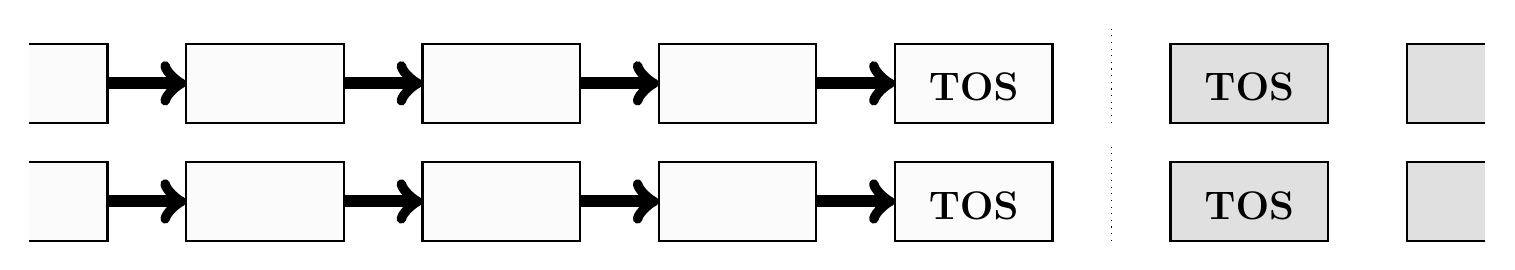
\begin{tikzpicture}
        \draw [thick, fill=gray!3]  (0,1.5) -- (1,1.5) -- (1,2.5) -- (0,2.5);%
        \draw [line width=1ex, ->]  (1,2)   -- (2,2);                %
        \draw [thick, fill=gray!3]  (2,1.5) rectangle (4,2.5);       %PS+3
        \draw [line width=1ex, ->]  (4,2)   -- (5,2);                %
        \draw [thick, fill=gray!3]  (5,1.5) rectangle (7,2.5);       %PS+2
        \draw [line width=1ex, ->]  (7,2)   -- (8,2);                %
        \draw [thick, fill=gray!3]  (8,1.5) rectangle (10,2.5);      %PS+1
        \draw [line width=1ex, ->]  (10,2)  -- (11,2);               %
        \draw [thick, fill=gray!3]  (11,1.5) rectangle (13,2.5);     %PS TOS
        \node at (12,1.95)          {\Large{\textbf{TOS}}};          %
        %\draw [line width=1ex, --] (13,2)  -- (14.5,2);             %
        \draw [dotted]              (13.75,1.5) -- (13.75,2.7);      %
        \draw [thick, fill=gray!24] (14.5,1.5) rectangle (16.5,2.5); %RS TOS
        \node at (15.5,1.95)        {\Large{\textbf{TOS}}};          %
        %\draw [line width=1ex, --] (16.5,2) -- (17.5,2);            % 
        \draw [thick, fill=gray!24] (18.5,1.5) -- (17.5,1.5) -- (17.5,2.5) -- (18.5,2.5);

        \draw [thick, fill=gray!3]  (0,0) -- (1,0) -- (1,1) -- (0,1);%
        \draw [line width=1ex, ->]  (1,0.5) -- (2,0.5);              %
        \draw [thick, fill=gray!3]  (2,0) rectangle (4,1);           %PS+3
        \draw [line width=1ex, ->]  (4,0.5) -- (5,0.5);              %
        \draw [thick, fill=gray!3]  (5,0) rectangle (7,1);           %PS+2
        \draw [line width=1ex, ->]  (7,0.5) -- (8,0.5);              %
        \draw [thick, fill=gray!3]  (8,0) rectangle (10,1);          %PS+1
        \draw [line width=1ex, ->]  (10,0.5) -- (11,0.5);            %
        \draw [thick, fill=gray!3]  (11,0) rectangle (13,1);         %PS TOS
        \node at (12,0.45)          {\Large{\textbf{TOS}}};          %
        %\draw [line width=1ex, --] (13,0.5)  -- (14.5,0.5);         %
        \draw [dotted]              (13.75,0) -- (13.75,1.2);        %
        \draw [thick, fill=gray!24] (14.5,0) rectangle (16.5,1);     %RS TOS
        \node at (15.5,0.45)        {\Large{\textbf{TOS}}};          %
        %\draw [line width=1ex, --] (16.5,0.5) -- (17.5,0.5);        % 
        \draw [thick, fill=gray!24] (18.5,0) -- (17.5,0) -- (17.5,1) -- (18.5,1);
      \end{tikzpicture}
    }} &
    \multicolumn{1}{m{4.25em}|}{
    \makecell[c]{ 
      \texttt{0x06A8} \\ 
      \texttt{0x06A8}
    }} \\ \hline

    %2DUP
    \texttt{2DUP} &
    ( x1 x2 -- x1 x2 x1 x2 ) &
    \multicolumn{1}{m{21.35em}|}{
    \scalebox{0.4} {
      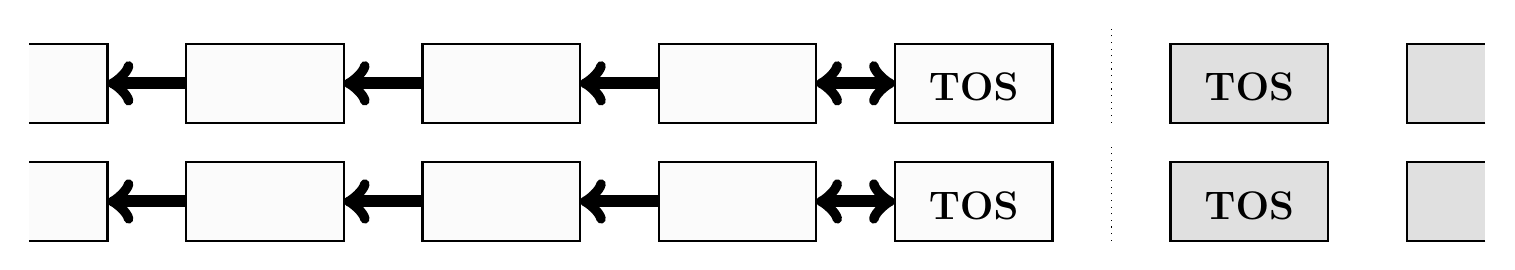
\begin{tikzpicture}
        \draw [thick, fill=gray!3]  (0,1.5) -- (1,1.5) -- (1,2.5) -- (0,2.5);%
        \draw [line width=1ex, <-]  (1,2)   -- (2,2);                %
        \draw [thick, fill=gray!3]  (2,1.5) rectangle (4,2.5);       %PS+3
        \draw [line width=1ex, <-]  (4,2)   -- (5,2);                %
        \draw [thick, fill=gray!3]  (5,1.5) rectangle (7,2.5);       %PS+2
        \draw [line width=1ex, <-]  (7,2)   -- (8,2);                %
        \draw [thick, fill=gray!3]  (8,1.5) rectangle (10,2.5);      %PS+1
        \draw [line width=1ex, <->] (10,2)  -- (11,2);               %
        \draw [thick, fill=gray!3]  (11,1.5) rectangle (13,2.5);     %PS TOS
        \node at (12,1.95)          {\Large{\textbf{TOS}}};          %
        %\draw [line width=1ex, --] (13,2)  -- (14.5,2);             %
        \draw [dotted]              (13.75,1.5) -- (13.75,2.7);      %
        \draw [thick, fill=gray!24] (14.5,1.5) rectangle (16.5,2.5); %RS TOS
        \node at (15.5,1.95)        {\Large{\textbf{TOS}}};          %
        %\draw [line width=1ex, --] (16.5,2) -- (17.5,2);            % 
        \draw [thick, fill=gray!24] (18.5,1.5) -- (17.5,1.5) -- (17.5,2.5) -- (18.5,2.5);

        \draw [thick, fill=gray!3]  (0,0) -- (1,0) -- (1,1) -- (0,1);%
        \draw [line width=1ex, <-]  (1,0.5) -- (2,0.5);              %
        \draw [thick, fill=gray!3]  (2,0) rectangle (4,1);           %PS+3
        \draw [line width=1ex, <-]  (4,0.5) -- (5,0.5);              %
        \draw [thick, fill=gray!3]  (5,0) rectangle (7,1);           %PS+2
        \draw [line width=1ex, <-]  (7,0.5) -- (8,0.5);              %
        \draw [thick, fill=gray!3]  (8,0) rectangle (10,1);          %PS+1
        \draw [line width=1ex, <->] (10,0.5) -- (11,0.5);            %
        \draw [thick, fill=gray!3]  (11,0) rectangle (13,1);         %PS TOS
        \node at (12,0.45)          {\Large{\textbf{TOS}}};          %
        %\draw [line width=1ex, --] (13,0.5)  -- (14.5,0.5);         %
        \draw [dotted]              (13.75,0) -- (13.75,1.2);        %
        \draw [thick, fill=gray!24] (14.5,0) rectangle (16.5,1);     %RS TOS
        \node at (15.5,0.45)        {\Large{\textbf{TOS}}};          %
        %\draw [line width=1ex, --] (16.5,0.5) -- (17.5,0.5);        % 
        \draw [thick, fill=gray!24] (18.5,0) -- (17.5,0) -- (17.5,1) -- (18.5,1);
      \end{tikzpicture}
    }} &
    \multicolumn{1}{m{4.25em}|}{
    \makecell[c]{ 
      \texttt{0x0758} \\
      \texttt{0x0758}
    }} \\ \hline

    %2SWAP
    \texttt{2SWAP} &
    ( x1 x2 x3 x4 -- x3 x4 x1 x2 ) &
    \multicolumn{1}{m{21.35em}|}{
    \scalebox{0.4} {
      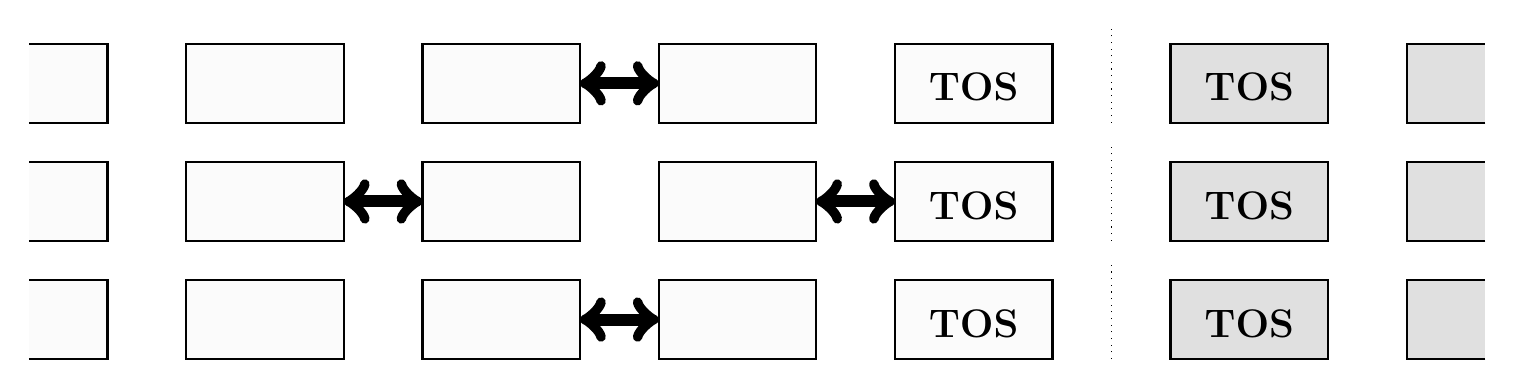
\begin{tikzpicture}
        \draw [thick, fill=gray!3]  (0,3) -- (1,3) -- (1,4) -- (0,4);%
        %\draw [line width=1ex, --] (1,3.5)   -- (2,3.5);            %
        \draw [thick, fill=gray!3]  (2,3) rectangle (4,4);           %PS+3
        %\draw [line width=1ex, --] (4,3.5)   -- (5,3.5);            %
        \draw [thick, fill=gray!3]  (5,3) rectangle (7,4);           %PS+2
        \draw [line width=1ex, <->] (7,3.5)   -- (8,3.5);            %
        \draw [thick, fill=gray!3]  (8,3) rectangle (10,4);          %PS+1
        %\draw [line width=1ex, --] (10,3.5)  -- (11,3.5);           %
        \draw [thick, fill=gray!3]  (11,3) rectangle (13,4);         %PS TOS
        \node at (12,3.45)          {\Large{\textbf{TOS}}};          %
        %\draw [line width=1ex, --] (13,3.5)  -- (14.5,3.5);         %
        \draw [dotted]              (13.75,3) -- (13.75,4.2);        %
        \draw [thick, fill=gray!24] (14.5,3) rectangle (16.5,4);     %RS TOS
        \node at (15.5,3.45)        {\Large{\textbf{TOS}}};          %
        %\draw [line width=1ex, --] (16.5,3.5) -- (17.5,3.5);        % 
        \draw [thick, fill=gray!24] (18.5,3)   -- (17.5,3) -- (17.5,4) -- (18.5,4);

        \draw [thick, fill=gray!3]  (0,1.5) -- (1,1.5) -- (1,2.5) -- (0,2.5);%
        %\draw [line width=1ex, --] (1,2)   -- (2,2);                %
        \draw [thick, fill=gray!3]  (2,1.5) rectangle (4,2.5);       %PS+3
        \draw [line width=1ex, <->] (4,2)   -- (5,2);                %
        \draw [thick, fill=gray!3]  (5,1.5) rectangle (7,2.5);       %PS+2
        %\draw [line width=1ex, --] (7,2)   -- (8,2);                %
        \draw [thick, fill=gray!3]  (8,1.5) rectangle (10,2.5);      %PS+1
        \draw [line width=1ex, <->] (10,2)  -- (11,2);               %
        \draw [thick, fill=gray!3]  (11,1.5) rectangle (13,2.5);     %PS TOS
        \node at (12,1.95)          {\Large{\textbf{TOS}}};          %
        %\draw [line width=1ex, --] (13,2)  -- (14.5,2);             %
        \draw [dotted]              (13.75,1.5) -- (13.75,2.7);      %
        \draw [thick, fill=gray!24] (14.5,1.5) rectangle (16.5,2.5); %RS TOS
        \node at (15.5,1.95)        {\Large{\textbf{TOS}}};          %
        %\draw [line width=1ex, --] (16.5,2) -- (17.5,2);            % 
        \draw [thick, fill=gray!24] (18.5,1.5) -- (17.5,1.5) -- (17.5,2.5) -- (18.5,2.5);

        \draw [thick, fill=gray!3]  (0,0) -- (1,0) -- (1,1) -- (0,1);%
        %\draw [line width=1ex, --] (1,0.5) -- (2,0.5);              %
        \draw [thick, fill=gray!3]  (2,0) rectangle (4,1);           %PS+3
        %\draw [line width=1ex, --] (4,0.5) -- (5,0.5);              %
        \draw [thick, fill=gray!3]  (5,0) rectangle (7,1);           %PS+2
        \draw [line width=1ex, <->] (7,0.5) -- (8,0.5);              %
        \draw [thick, fill=gray!3]  (8,0) rectangle (10,1);          %PS+1
        %\draw [line width=1ex, --] (10,0.5) -- (11,0.5);            %
        \draw [thick, fill=gray!3]  (11,0) rectangle (13,1);         %PS TOS
        \node at (12,0.45)          {\Large{\textbf{TOS}}};          %
        %\draw [line width=1ex, --] (13,0.5)  -- (14.5,0.5);         %
        \draw [dotted]              (13.75,0) -- (13.75,1.2);        %
        \draw [thick, fill=gray!24] (14.5,0) rectangle (16.5,1);     %RS TOS
        \node at (15.5,0.45)        {\Large{\textbf{TOS}}};          %
        %\draw [line width=1ex, --] (16.5,0.5) -- (17.5,0.5);        % 
        \draw [thick, fill=gray!24] (18.5,0) -- (17.5,0) -- (17.5,1) -- (18.5,1);
      \end{tikzpicture}
    }} &
    \multicolumn{1}{m{4.25em}|}{
    \makecell[c]{ 
      \texttt{0x0460} \\ 
      \texttt{0x0598} \\ 
      \texttt{0x0460}
    }} \\ \hline

    %2OVER
    \texttt{2OVER} &
    ( x1 x2 x3 x4 -- x1 x2 x3 x4 x1 x2 ) &
    \multicolumn{1}{m{21.35em}|}{
    \scalebox{0.4} {
      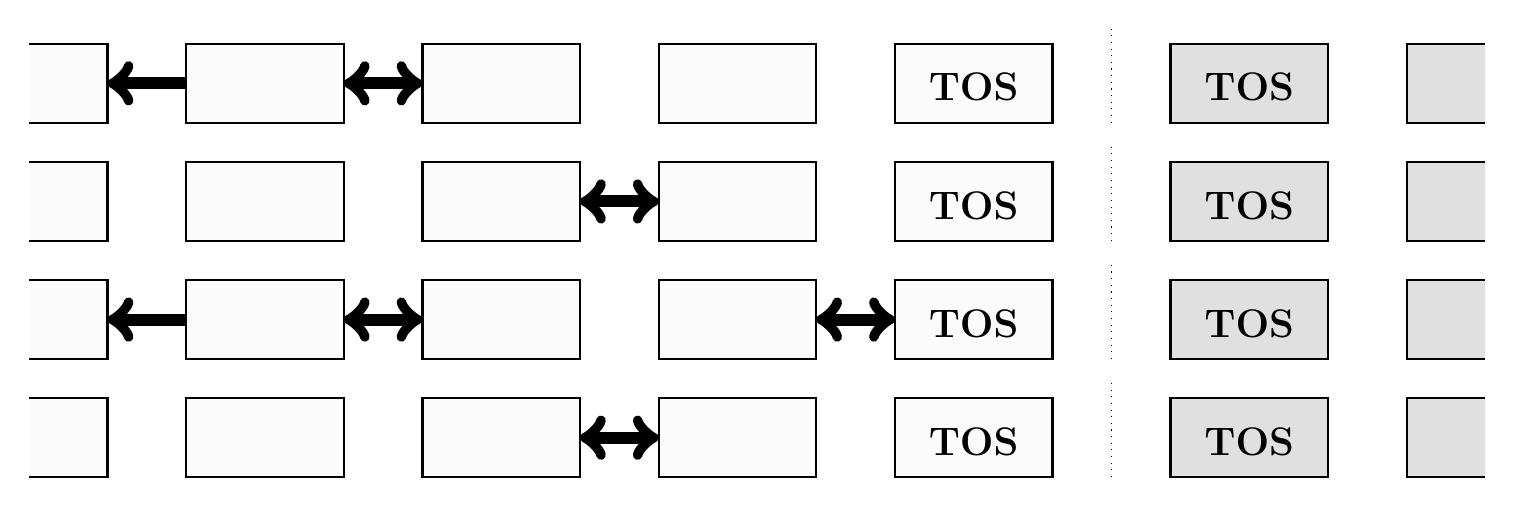
\begin{tikzpicture}
        \draw [thick, fill=gray!3]  (0,4.5) -- (1,4.5) -- (1,5.5) -- (0,5.5);%
        \draw [line width=1ex, <-]  (1,5)   -- (2,5);                %
        \draw [thick, fill=gray!3]  (2,4.5) rectangle (4,5.5);       %PS+3
        \draw [line width=1ex, <->] (4,5)   -- (5,5);                %
        \draw [thick, fill=gray!3]  (5,4.5) rectangle (7,5.5);       %PS+2
        %\draw [line width=1ex, --] (7,5)   -- (8,5);                %
        \draw [thick, fill=gray!3]  (8,4.5) rectangle (10,5.5);      %PS+1
        %\draw [line width=1ex, --] (10,5)  -- (11,5);               %
        \draw [thick, fill=gray!3]  (11,4.5) rectangle (13,5.5);     %PS TOS
        \node at (12,4.95)          {\Large{\textbf{TOS}}};          %
        %\draw [line width=1ex, --] (13,5)  -- (14.5,5);             %
        \draw [dotted]              (13.75,4.5) -- (13.75,5.7);      %
        \draw [thick, fill=gray!24] (14.5,4.5) rectangle (16.5,5.5); %RS TOS
        \node at (15.5,4.95)        {\Large{\textbf{TOS}}};          %
        %\draw [line width=1ex, --] (16.5,5) -- (17.5,5);            % 
        \draw [thick, fill=gray!24] (18.5,4.5) -- (17.5,4.5) -- (17.5,5.5) -- (18.5,5.5);

        \draw [thick, fill=gray!3]  (0,3) -- (1,3) -- (1,4) -- (0,4);%
        %\draw [line width=1ex, --] (1,3.5)   -- (2,3.5);            %
        \draw [thick, fill=gray!3]  (2,3) rectangle (4,4);           %PS+3
        %\draw [line width=1ex, --] (4,3.5)   -- (5,3.5);            %
        \draw [thick, fill=gray!3]  (5,3) rectangle (7,4);           %PS+2
        \draw [line width=1ex, <->] (7,3.5)   -- (8,3.5);            %
        \draw [thick, fill=gray!3]  (8,3) rectangle (10,4);          %PS+1
        %\draw [line width=1ex, --] (10,3.5)  -- (11,3.5);           %
        \draw [thick, fill=gray!3]  (11,3) rectangle (13,4);         %PS TOS
        \node at (12,3.45)          {\Large{\textbf{TOS}}};          %
        %\draw [line width=1ex, --] (13,3.5)  -- (14.5,3.5);         %
        \draw [dotted]              (13.75,3) -- (13.75,4.2);        %
        \draw [thick, fill=gray!24] (14.5,3) rectangle (16.5,4);     %RS TOS
        \node at (15.5,3.45)        {\Large{\textbf{TOS}}};          %
        %\draw [line width=1ex, --] (16.5,3.5) -- (17.5,3.5);        % 
        \draw [thick, fill=gray!24] (18.5,3)   -- (17.5,3) -- (17.5,4) -- (18.5,4);

        \draw [thick, fill=gray!3]  (0,1.5) -- (1,1.5) -- (1,2.5) -- (0,2.5);%
        \draw [line width=1ex, <-]  (1,2)   -- (2,2);                %
        \draw [thick, fill=gray!3]  (2,1.5) rectangle (4,2.5);       %PS+3
        \draw [line width=1ex, <->] (4,2)   -- (5,2);                %
        \draw [thick, fill=gray!3]  (5,1.5) rectangle (7,2.5);       %PS+2
        %\draw [line width=1ex, --] (7,2)   -- (8,2);                %
        \draw [thick, fill=gray!3]  (8,1.5) rectangle (10,2.5);      %PS+1
        \draw [line width=1ex, <->] (10,2)  -- (11,2);               %
        \draw [thick, fill=gray!3]  (11,1.5) rectangle (13,2.5);     %PS TOS
        \node at (12,1.95)          {\Large{\textbf{TOS}}};          %
        %\draw [line width=1ex, --] (13,2)  -- (14.5,2);             %
        \draw [dotted]              (13.75,1.5) -- (13.75,2.7);      %
        \draw [thick, fill=gray!24] (14.5,1.5) rectangle (16.5,2.5); %RS TOS
        \node at (15.5,1.95)        {\Large{\textbf{TOS}}};          %
        %\draw [line width=1ex, --] (16.5,2) -- (17.5,2);            % 
        \draw [thick, fill=gray!24] (18.5,1.5) -- (17.5,1.5) -- (17.5,2.5) -- (18.5,2.5);

        \draw [thick, fill=gray!3]  (0,0) -- (1,0) -- (1,1) -- (0,1);%
        %\draw [line width=1ex, --] (1,0.5) -- (2,0.5);              %
        \draw [thick, fill=gray!3]  (2,0) rectangle (4,1);           %PS+3
        %\draw [line width=1ex, --] (4,0.5) -- (5,0.5);              %
        \draw [thick, fill=gray!3]  (5,0) rectangle (7,1);           %PS+2
        \draw [line width=1ex, <->] (7,0.5) -- (8,0.5);              %
        \draw [thick, fill=gray!3]  (8,0) rectangle (10,1);          %PS+1
        %\draw [line width=1ex, --] (10,0.5) -- (11,0.5);            %
        \draw [thick, fill=gray!3]  (11,0) rectangle (13,1);         %PS TOS
        \node at (12,0.45)          {\Large{\textbf{TOS}}};          %
        %\draw [line width=1ex, --] (13,0.5)  -- (14.5,0.5);         %
        \draw [dotted]              (13.75,0) -- (13.75,1.2);        %
        \draw [thick, fill=gray!24] (14.5,0) rectangle (16.5,1);     %RS TOS
        \node at (15.5,0.45)        {\Large{\textbf{TOS}}};          %
        %\draw [line width=1ex, --] (16.5,0.5) -- (17.5,0.5);        % 
        \draw [thick, fill=gray!24] (18.5,0) -- (17.5,0) -- (17.5,1) -- (18.5,1);
      \end{tikzpicture}
    }} &
    \multicolumn{1}{m{4.25em}|}{
    \makecell[c]{ 
      \texttt{0x0780} \\ 
      \texttt{0x0460} \\ 
      \texttt{0x0798} \\ 
      \texttt{0x0460}
    }} \\ \hline

    %2NIP
    \texttt{2NIP} &
    ( x1 x2 x3 x4 -- x3 x4 ) &
    \multicolumn{1}{m{21.35em}|}{
    \scalebox{0.4} {
      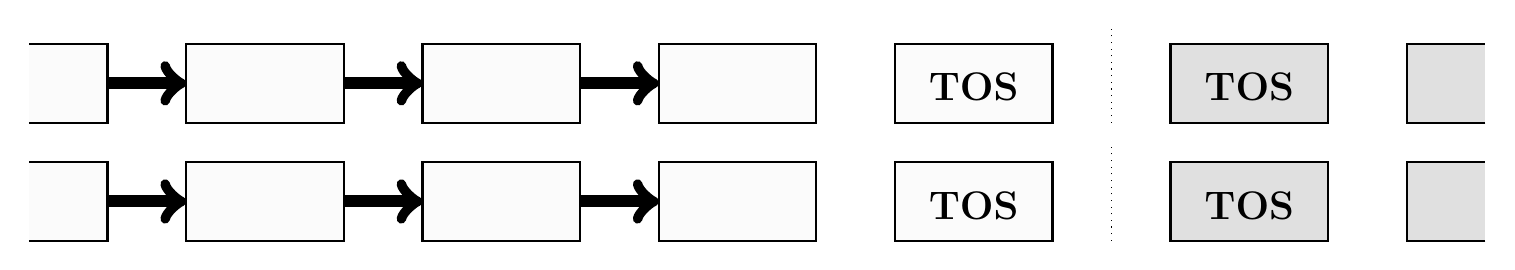
\begin{tikzpicture}
        \draw [thick, fill=gray!3]  (0,1.5) -- (1,1.5) -- (1,2.5) -- (0,2.5);%
        \draw [line width=1ex, ->]  (1,2)   -- (2,2);                %
        \draw [thick, fill=gray!3]  (2,1.5) rectangle (4,2.5);       %PS+3
        \draw [line width=1ex, ->]  (4,2)   -- (5,2);                %
        \draw [thick, fill=gray!3]  (5,1.5) rectangle (7,2.5);       %PS+2
        \draw [line width=1ex, ->]  (7,2)   -- (8,2);                %
        \draw [thick, fill=gray!3]  (8,1.5) rectangle (10,2.5);      %PS+1
        %\draw [line width=1ex, --] (10,2)  -- (11,2);               %
        \draw [thick, fill=gray!3]  (11,1.5) rectangle (13,2.5);     %PS TOS
        \node at (12,1.95)          {\Large{\textbf{TOS}}};          %
        %\draw [line width=1ex, --] (13,2)  -- (14.5,2);             %
        \draw [dotted]              (13.75,1.5) -- (13.75,2.7);      %
        \draw [thick, fill=gray!24] (14.5,1.5) rectangle (16.5,2.5); %RS TOS
        \node at (15.5,1.95)        {\Large{\textbf{TOS}}};          %
        %\draw [line width=1ex, --] (16.5,2) -- (17.5,2);            % 
        \draw [thick, fill=gray!24] (18.5,1.5) -- (17.5,1.5) -- (17.5,2.5) -- (18.5,2.5);

        \draw [thick, fill=gray!3]  (0,0) -- (1,0) -- (1,1) -- (0,1);%
        \draw [line width=1ex, ->]  (1,0.5) -- (2,0.5);              %
        \draw [thick, fill=gray!3]  (2,0) rectangle (4,1);           %PS+3
        \draw [line width=1ex, ->]  (4,0.5) -- (5,0.5);              %
        \draw [thick, fill=gray!3]  (5,0) rectangle (7,1);           %PS+2
        \draw [line width=1ex, ->]  (7,0.5) -- (8,0.5);              %
        \draw [thick, fill=gray!3]  (8,0) rectangle (10,1);          %PS+1
        %\draw [line width=1ex, --] (10,0.5) -- (11,0.5);            %
        \draw [thick, fill=gray!3]  (11,0) rectangle (13,1);         %PS TOS
        \node at (12,0.45)          {\Large{\textbf{TOS}}};          %
        %\draw [line width=1ex, --] (13,0.5)  -- (14.5,0.5);         %
        \draw [dotted]              (13.75,0) -- (13.75,1.2);        %
        \draw [thick, fill=gray!24] (14.5,0) rectangle (16.5,1);     %RS TOS
        \node at (15.5,0.45)        {\Large{\textbf{TOS}}};          %
        %\draw [line width=1ex, --] (16.5,0.5) -- (17.5,0.5);        % 
        \draw [thick, fill=gray!24] (18.5,0) -- (17.5,0) -- (17.5,1) -- (18.5,1);
      \end{tikzpicture}
    }} &
    \multicolumn{1}{m{4.25em}|}{
    \makecell[c]{ 
      \texttt{0x06A0} \\ 
      \texttt{0x06A0}
    }} \\ \hline

    %2TUCK
    \texttt{2TUCK} &
    ( x1 x2 x3 x4 -- x3 x4 x1 x2 x3 x4 ) &
    \multicolumn{1}{m{21.35em}|}{
    \scalebox{0.4} {
      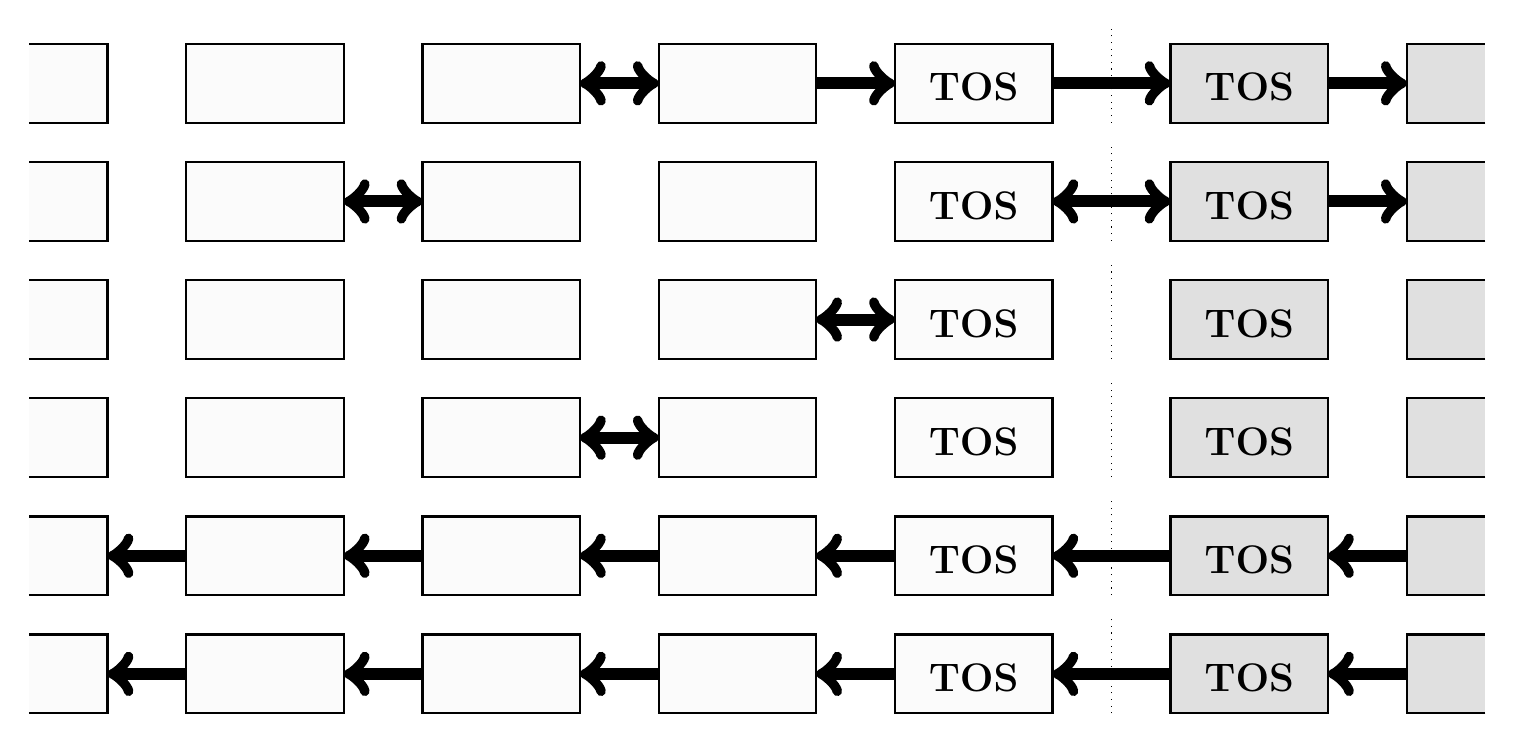
\begin{tikzpicture}
        \draw [thick, fill=gray!3]  (0,7.5) -- (1,7.5) -- (1,8.5) -- (0,8.5);%
        %\draw [line width=1ex, --] (1,8)   -- (2,8);                %
        \draw [thick, fill=gray!3]  (2,7.5) rectangle (4,8.5);       %PS+3
        %\draw [line width=1ex, --] (4,8)   -- (5,8);                %
        \draw [thick, fill=gray!3]  (5,7.5) rectangle (7,8.5);       %PS+2
        \draw [line width=1ex, <->] (7,8)   -- (8,8);                %
        \draw [thick, fill=gray!3]  (8,7.5) rectangle (10,8.5);      %PS+1
        \draw [line width=1ex, ->]  (10,8)  -- (11,8);               %
        \draw [thick, fill=gray!3]  (11,7.5) rectangle (13,8.5);     %PS TOS
        \node at (12,7.95)          {\Large{\textbf{TOS}}};          %
        \draw [line width=1ex, ->]  (13,8)  -- (14.5,8);             %
        \draw [dotted]              (13.75,7.5) -- (13.75,8.7);      %
        \draw [thick, fill=gray!24] (14.5,7.5) rectangle (16.5,8.5); %RS TOS
        \node at (15.5,7.95)        {\Large{\textbf{TOS}}};          %
        \draw [line width=1ex, ->]  (16.5,8) -- (17.5,8);            % 
        \draw [thick, fill=gray!24] (18.5,7.5) -- (17.5,7.5) -- (17.5,8.5) -- (18.5,8.5);

        \draw [thick, fill=gray!3]  (0,6) -- (1,6) -- (1,7) -- (0,7);%
        %\draw [line width=1ex, --] (1,6.5)   -- (2,6.5);            %
        \draw [thick, fill=gray!3]  (2,6) rectangle (4,7);           %PS+3
        \draw [line width=1ex, <->] (4,6.5)   -- (5,6.5);            %
        \draw [thick, fill=gray!3]  (5,6) rectangle (7,7);           %PS+2
        %\draw [line width=1ex, --] (7,6.5)   -- (8,6.5);            %
        \draw [thick, fill=gray!3]  (8,6) rectangle (10,7);          %PS+1
        %\draw [line width=1ex, --] (10,6.5)  -- (11,6.5);           %
        \draw [thick, fill=gray!3]  (11,6) rectangle (13,7);         %PS TOS
        \node at (12,6.45)          {\Large{\textbf{TOS}}};          %
        \draw [line width=1ex, <->] (13,6.5)  -- (14.5,6.5);         %
        \draw [dotted]              (13.75,6) -- (13.75,7.2);        %
        \draw [thick, fill=gray!24] (14.5,6) rectangle (16.5,7);     %RS TOS
        \node at (15.5,6.45)        {\Large{\textbf{TOS}}};          %
        \draw [line width=1ex, ->]  (16.5,6.5) -- (17.5,6.5);         % 
        \draw [thick, fill=gray!24] (18.5,6)   -- (17.5,6) -- (17.5,7) -- (18.5,7);

        \draw [thick, fill=gray!3]  (0,4.5) -- (1,4.5) -- (1,5.5) -- (0,5.5);%
        %\draw [line width=1ex, --] (1,5)   -- (2,5);                %
        \draw [thick, fill=gray!3]  (2,4.5) rectangle (4,5.5);       %PS+3
        %\draw [line width=1ex, --] (4,5)   -- (5,5);                %
        \draw [thick, fill=gray!3]  (5,4.5) rectangle (7,5.5);       %PS+2
        %\draw [line width=1ex, --] (7,5)   -- (8,5);                %
        \draw [thick, fill=gray!3]  (8,4.5) rectangle (10,5.5);      %PS+1
        \draw [line width=1ex, <->] (10,5)  -- (11,5);               %
        \draw [thick, fill=gray!3]  (11,4.5) rectangle (13,5.5);     %PS TOS
        \node at (12,4.95)          {\Large{\textbf{TOS}}};          %
        %\draw [line width=1ex, --] (13,5)  -- (14.5,5);             %
        \draw [dotted]              (13.75,4.5) -- (13.75,5.7);      %
        \draw [thick, fill=gray!24] (14.5,4.5) rectangle (16.5,5.5); %RS TOS
        \node at (15.5,4.95)        {\Large{\textbf{TOS}}};          %
        %\draw [line width=1ex, --] (16.5,5) -- (17.5,5);            % 
        \draw [thick, fill=gray!24] (18.5,4.5) -- (17.5,4.5) -- (17.5,5.5) -- (18.5,5.5);

        \draw [thick, fill=gray!3]  (0,3) -- (1,3) -- (1,4) -- (0,4);%
        %\draw [line width=1ex, --] (1,3.5)   -- (2,3.5);            %
        \draw [thick, fill=gray!3]  (2,3) rectangle (4,4);           %PS+3
        %\draw [line width=1ex, --] (4,3.5)   -- (5,3.5);            %
        \draw [thick, fill=gray!3]  (5,3) rectangle (7,4);           %PS+2
        \draw [line width=1ex, <->] (7,3.5)   -- (8,3.5);            %
        \draw [thick, fill=gray!3]  (8,3) rectangle (10,4);          %PS+1
        %\draw [line width=1ex, --] (10,3.5)  -- (11,3.5);           %
        \draw [thick, fill=gray!3]  (11,3) rectangle (13,4);         %PS TOS
        \node at (12,3.45)          {\Large{\textbf{TOS}}};          %
        %\draw [line width=1ex, --] (13,3.5)  -- (14.5,3.5);         %
        \draw [dotted]              (13.75,3) -- (13.75,4.2);        %
        \draw [thick, fill=gray!24] (14.5,3) rectangle (16.5,4);     %RS TOS
        \node at (15.5,3.45)        {\Large{\textbf{TOS}}};          %
        %\draw [line width=1ex, --] (16.5,3.5) -- (17.5,3.5);        % 
        \draw [thick, fill=gray!24] (18.5,3)   -- (17.5,3) -- (17.5,4) -- (18.5,4);

        \draw [thick, fill=gray!3]  (0,1.5) -- (1,1.5) -- (1,2.5) -- (0,2.5);%
        \draw [line width=1ex, <-]  (1,2)   -- (2,2);                %
        \draw [thick, fill=gray!3]  (2,1.5) rectangle (4,2.5);       %PS+3
        \draw [line width=1ex, <-]  (4,2)   -- (5,2);                %
        \draw [thick, fill=gray!3]  (5,1.5) rectangle (7,2.5);       %PS+2
        \draw [line width=1ex, <-]  (7,2)   -- (8,2);                %
        \draw [thick, fill=gray!3]  (8,1.5) rectangle (10,2.5);      %PS+1
        \draw [line width=1ex, <-]  (10,2)  -- (11,2);               %
        \draw [thick, fill=gray!3]  (11,1.5) rectangle (13,2.5);     %PS TOS
        \node at (12,1.95)          {\Large{\textbf{TOS}}};          %
        \draw [line width=1ex, <-]  (13,2)  -- (14.5,2);             %
        \draw [dotted]              (13.75,1.5) -- (13.75,2.7);      %
        \draw [thick, fill=gray!24] (14.5,1.5) rectangle (16.5,2.5); %RS TOS
        \node at (15.5,1.95)        {\Large{\textbf{TOS}}};          %
        \draw [line width=1ex, <-]  (16.5,2) -- (17.5,2);            % 
        \draw [thick, fill=gray!24] (18.5,1.5) -- (17.5,1.5) -- (17.5,2.5) -- (18.5,2.5);

        \draw [thick, fill=gray!3]  (0,0) -- (1,0) -- (1,1) -- (0,1);%
        \draw [line width=1ex, <-]  (1,0.5) -- (2,0.5);              %
        \draw [thick, fill=gray!3]  (2,0) rectangle (4,1);           %PS+3
        \draw [line width=1ex, <-]  (4,0.5) -- (5,0.5);              %
        \draw [thick, fill=gray!3]  (5,0) rectangle (7,1);           %PS+2
        \draw [line width=1ex, <-]  (7,0.5) -- (8,0.5);              %
        \draw [thick, fill=gray!3]  (8,0) rectangle (10,1);          %PS+1
        \draw [line width=1ex, <-]  (10,0.5) -- (11,0.5);            %
        \draw [thick, fill=gray!3]  (11,0) rectangle (13,1);         %PS TOS
        \node at (12,0.45)          {\Large{\textbf{TOS}}};          %
        \draw [line width=1ex, <-]  (13,0.5)  -- (14.5,0.5);         %
        \draw [dotted]              (13.75,0) -- (13.75,1.2);        %
        \draw [thick, fill=gray!24] (14.5,0) rectangle (16.5,1);     %RS TOS
        \node at (15.5,0.45)        {\Large{\textbf{TOS}}};          %
        \draw [line width=1ex, <-]  (16.5,0.5) -- (17.5,0.5);        % 
        \draw [thick, fill=gray!24] (18.5,0) -- (17.5,0) -- (17.5,1) -- (18.5,1);
      \end{tikzpicture}
    }} &
    \multicolumn{1}{m{4.25em}|}{
    \makecell[c]{ 
      \texttt{0x046B} \\ 
      \texttt{0x0587} \\ 
      \texttt{0x0418} \\ 
      \texttt{0x0460} \\ 
      \texttt{0x0755} \\ 
      \texttt{0x0755}
    }} \\ \hline

    %2ROT
    \texttt{2ROT} &
    ( x1 x2 x3 x4 x5 x6 -- x3 x4 x5 x6 x1 x2 ) &
    \multicolumn{1}{m{21.35em}|}{
    \scalebox{0.4} {
      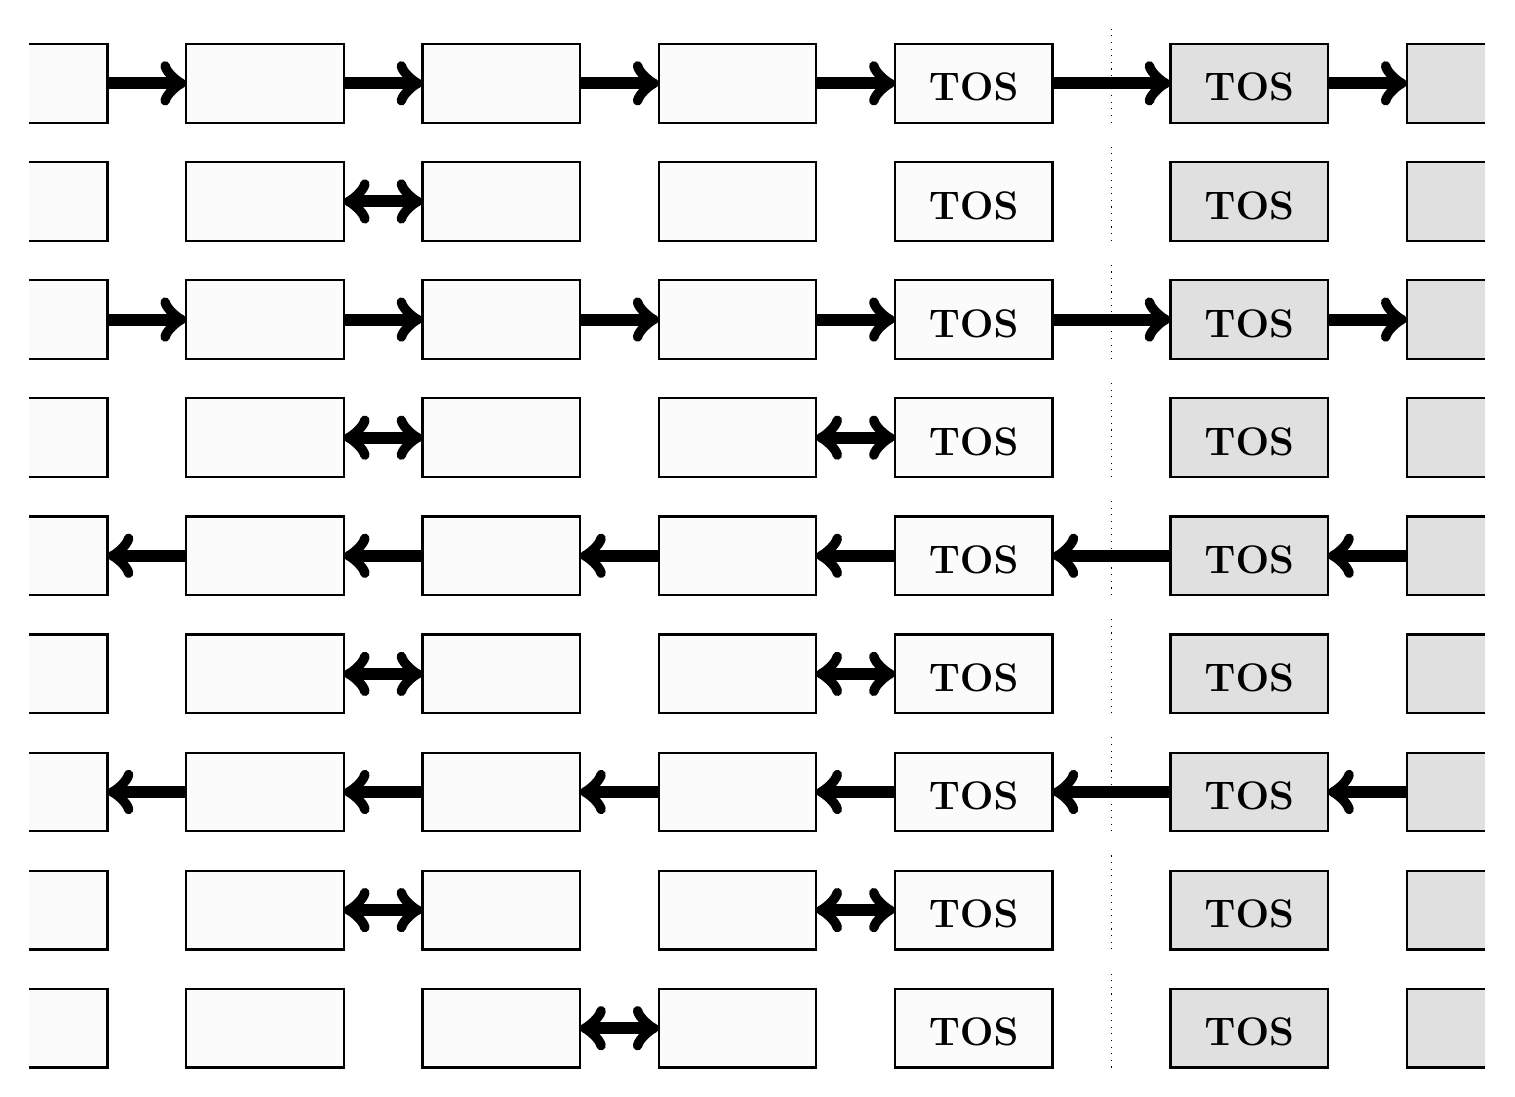
\begin{tikzpicture}
        \draw [thick, fill=gray!3]  (0,12) -- (1,12) -- (1,13) -- (0,13);%
        \draw [line width=1ex, ->]  (1,12.5)   -- (2,12.5);          %
        \draw [thick, fill=gray!3]  (2,12) rectangle (4,13);         %PS+3
        \draw [line width=1ex, ->]  (4,12.5)   -- (5,12.5);          %
        \draw [thick, fill=gray!3]  (5,12) rectangle (7,13);         %PS+2
        \draw [line width=1ex, ->]  (7,12.5)   -- (8,12.5);          %
        \draw [thick, fill=gray!3]  (8,12) rectangle (10,13);        %PS+1
        \draw [line width=1ex, ->]  (10,12.5)  -- (11,12.5);         %
        \draw [thick, fill=gray!3]  (11,12) rectangle (13,13);       %PS TOS
        \node at (12,12.45)         {\Large{\textbf{TOS}}};          %
        \draw [line width=1ex, ->]  (13,12.5)  -- (14.5,12.5);       %
        \draw [dotted]              (13.75,12) -- (13.75,13.2);      %
        \draw [thick, fill=gray!24] (14.5,12) rectangle (16.5,13);   %RS TOS
        \node at (15.5,12.45)       {\Large{\textbf{TOS}}};          %
        \draw [line width=1ex, ->]  (16.5,12.5) -- (17.5,12.5);      % 
        \draw [thick, fill=gray!24] (18.5,12)   -- (17.5,12) -- (17.5,13) -- (18.5,13);

        \draw [thick, fill=gray!3]  (0,10.5) -- (1,10.5) -- (1,11.5) -- (0,11.5);%
        %\draw [line width=1ex, --] (1,11)   -- (2,11);              %
        \draw [thick, fill=gray!3]  (2,10.5) rectangle (4,11.5);     %PS+3
        \draw [line width=1ex, <->] (4,11)   -- (5,11);              %
        \draw [thick, fill=gray!3]  (5,10.5) rectangle (7,11.5);     %PS+2
        %\draw [line width=1ex, --] (7,11)   -- (8,11);              %
        \draw [thick, fill=gray!3]  (8,10.5) rectangle (10,11.5);    %PS+1
        %\draw [line width=1ex, --] (10,11)  -- (11,11);             %
        \draw [thick, fill=gray!3]  (11,10.5) rectangle (13,11.5);   %PS TOS
        \node at (12,10.95)         {\Large{\textbf{TOS}}};          %
        %\draw [line width=1ex, --] (13,11)  -- (14.5,11);           %
        \draw [dotted]              (13.75,10.5) -- (13.75,11.7);    %
        \draw [thick, fill=gray!24] (14.5,10.5) rectangle (16.5,11.5);%RS TOS
        \node at (15.5,10.95)       {\Large{\textbf{TOS}}};          %
        %\draw [line width=1ex, --] (16.5,11) -- (17.5,11);          % 
        \draw [thick, fill=gray!24] (18.5,10.5) -- (17.5,10.5) -- (17.5,11.5) -- (18.5,11.5);

        \draw [thick, fill=gray!3]  (0,9) -- (1,9) -- (1,10) -- (0,10);%
        \draw [line width=1ex, ->]  (1,9.5)   -- (2,9.5);            %
        \draw [thick, fill=gray!3]  (2,9) rectangle (4,10);          %PS+3
        \draw [line width=1ex, ->]  (4,9.5)   -- (5,9.5);            %
        \draw [thick, fill=gray!3]  (5,9) rectangle (7,10);          %PS+2
        \draw [line width=1ex, ->]  (7,9.5)   -- (8,9.5);            %
        \draw [thick, fill=gray!3]  (8,9) rectangle (10,10);         %PS+1
        \draw [line width=1ex, ->]  (10,9.5)  -- (11,9.5);           %
        \draw [thick, fill=gray!3]  (11,9) rectangle (13,10);        %PS TOS
        \node at (12,9.45)          {\Large{\textbf{TOS}}};          %
        \draw [line width=1ex, ->]  (13,9.5)  -- (14.5,9.5);         %
        \draw [dotted]              (13.75,9) -- (13.75,10.2);       %
        \draw [thick, fill=gray!24] (14.5,9) rectangle (16.5,10);    %RS TOS
        \node at (15.5,9.45)        {\Large{\textbf{TOS}}};          %
        \draw [line width=1ex, ->]  (16.5,9.5) -- (17.5,9.5);        % 
        \draw [thick, fill=gray!24] (18.5,9)   -- (17.5,9) -- (17.5,10) -- (18.5,10);

        \draw [thick, fill=gray!3]  (0,7.5) -- (1,7.5) -- (1,8.5) -- (0,8.5);%
        %\draw [line width=1ex, --] (1,8)   -- (2,8);                %
        \draw [thick, fill=gray!3]  (2,7.5) rectangle (4,8.5);       %PS+3
        \draw [line width=1ex, <->] (4,8)   -- (5,8);                %
        \draw [thick, fill=gray!3]  (5,7.5) rectangle (7,8.5);       %PS+2
        %\draw [line width=1ex, --] (7,8)   -- (8,8);                %
        \draw [thick, fill=gray!3]  (8,7.5) rectangle (10,8.5);      %PS+1
        \draw [line width=1ex, <->] (10,8)  -- (11,8);               %
        \draw [thick, fill=gray!3]  (11,7.5) rectangle (13,8.5);     %PS TOS
        \node at (12,7.95)          {\Large{\textbf{TOS}}};          %
        %\draw [line width=1ex, --] (13,8)  -- (14.5,8);             %
        \draw [dotted]              (13.75,7.5) -- (13.75,8.7);      %
        \draw [thick, fill=gray!24] (14.5,7.5) rectangle (16.5,8.5); %RS TOS
        \node at (15.5,7.95)        {\Large{\textbf{TOS}}};          %
        %\draw [line width=1ex, --] (16.5,8) -- (17.5,8);            % 
        \draw [thick, fill=gray!24] (18.5,7.5) -- (17.5,7.5) -- (17.5,8.5) -- (18.5,8.5);

        \draw [thick, fill=gray!3]  (0,6) -- (1,6) -- (1,7) -- (0,7);%
        \draw [line width=1ex, <-]  (1,6.5)   -- (2,6.5);            %
        \draw [thick, fill=gray!3]  (2,6) rectangle (4,7);           %PS+3
        \draw [line width=1ex, <-]  (4,6.5)   -- (5,6.5);            %
        \draw [thick, fill=gray!3]  (5,6) rectangle (7,7);           %PS+2
        \draw [line width=1ex, <-]  (7,6.5)   -- (8,6.5);            %
        \draw [thick, fill=gray!3]  (8,6) rectangle (10,7);          %PS+1
        \draw [line width=1ex, <-]  (10,6.5)  -- (11,6.5);           %
        \draw [thick, fill=gray!3]  (11,6) rectangle (13,7);         %PS TOS
        \node at (12,6.45)          {\Large{\textbf{TOS}}};          %
        \draw [line width=1ex, <-]  (13,6.5)  -- (14.5,6.5);         %
        \draw [dotted]              (13.75,6) -- (13.75,7.2);        %
        \draw [thick, fill=gray!24] (14.5,6) rectangle (16.5,7);     %RS TOS
        \node at (15.5,6.45)        {\Large{\textbf{TOS}}};          %
        \draw [line width=1ex, <-]  (16.5,6.5) -- (17.5,6.5);        % 
        \draw [thick, fill=gray!24] (18.5,6)   -- (17.5,6) -- (17.5,7) -- (18.5,7);

        \draw [thick, fill=gray!3]  (0,4.5) -- (1,4.5) -- (1,5.5) -- (0,5.5);%
        %\draw [line width=1ex, --] (1,5)   -- (2,5);                %
        \draw [thick, fill=gray!3]  (2,4.5) rectangle (4,5.5);       %PS+3
        \draw [line width=1ex, <->] (4,5)   -- (5,5);                %
        \draw [thick, fill=gray!3]  (5,4.5) rectangle (7,5.5);       %PS+2
        %\draw [line width=1ex, --] (7,5)   -- (8,5);                %
        \draw [thick, fill=gray!3]  (8,4.5) rectangle (10,5.5);      %PS+1
        \draw [line width=1ex, <->] (10,5)  -- (11,5);               %
        \draw [thick, fill=gray!3]  (11,4.5) rectangle (13,5.5);     %PS TOS
        \node at (12,4.95)          {\Large{\textbf{TOS}}};          %
        %\draw [line width=1ex, --] (13,5)  -- (14.5,5);             %
        \draw [dotted]              (13.75,4.5) -- (13.75,5.7);      %
        \draw [thick, fill=gray!24] (14.5,4.5) rectangle (16.5,5.5); %RS TOS
        \node at (15.5,4.95)        {\Large{\textbf{TOS}}};          %
        %\draw [line width=1ex, --] (16.5,5) -- (17.5,5);            % 
        \draw [thick, fill=gray!24] (18.5,4.5) -- (17.5,4.5) -- (17.5,5.5) -- (18.5,5.5);

        \draw [thick, fill=gray!3]  (0,3) -- (1,3) -- (1,4) -- (0,4);%
        \draw [line width=1ex, <-]  (1,3.5)   -- (2,3.5);            %
        \draw [thick, fill=gray!3]  (2,3) rectangle (4,4);           %PS+3
        \draw [line width=1ex, <-]  (4,3.5)   -- (5,3.5);            %
        \draw [thick, fill=gray!3]  (5,3) rectangle (7,4);           %PS+2
        \draw [line width=1ex, <-]  (7,3.5)   -- (8,3.5);            %
        \draw [thick, fill=gray!3]  (8,3) rectangle (10,4);          %PS+1
        \draw [line width=1ex, <-]  (10,3.5)  -- (11,3.5);           %
        \draw [thick, fill=gray!3]  (11,3) rectangle (13,4);         %PS TOS
        \node at (12,3.45)          {\Large{\textbf{TOS}}};          %
        \draw [line width=1ex, <-]  (13,3.5)  -- (14.5,3.5);         %
        \draw [dotted]              (13.75,3) -- (13.75,4.2);        %
        \draw [thick, fill=gray!24] (14.5,3) rectangle (16.5,4);     %RS TOS
        \node at (15.5,3.45)        {\Large{\textbf{TOS}}};          %
        \draw [line width=1ex, <-]  (16.5,3.5) -- (17.5,3.5);        % 
        \draw [thick, fill=gray!24] (18.5,3)   -- (17.5,3) -- (17.5,4) -- (18.5,4);

        \draw [thick, fill=gray!3]  (0,1.5) -- (1,1.5) -- (1,2.5) -- (0,2.5);%
        %\draw [line width=1ex, --] (1,2)   -- (2,2);                %
        \draw [thick, fill=gray!3]  (2,1.5) rectangle (4,2.5);       %PS+3
        \draw [line width=1ex, <->] (4,2)   -- (5,2);                %
        \draw [thick, fill=gray!3]  (5,1.5) rectangle (7,2.5);       %PS+2
        %\draw [line width=1ex, --] (7,2)   -- (8,2);                %
        \draw [thick, fill=gray!3]  (8,1.5) rectangle (10,2.5);      %PS+1
        \draw [line width=1ex, <->] (10,2)  -- (11,2);               %
        \draw [thick, fill=gray!3]  (11,1.5) rectangle (13,2.5);     %PS TOS
        \node at (12,1.95)          {\Large{\textbf{TOS}}};          %
        %\draw [line width=1ex, --] (13,2)  -- (14.5,2);             %
        \draw [dotted]              (13.75,1.5) -- (13.75,2.7);      %
        \draw [thick, fill=gray!24] (14.5,1.5) rectangle (16.5,2.5); %RS TOS
        \node at (15.5,1.95)        {\Large{\textbf{TOS}}};          %
        %\draw [line width=1ex, --] (16.5,2) -- (17.5,2);            % 
        \draw [thick, fill=gray!24] (18.5,1.5) -- (17.5,1.5) -- (17.5,2.5) -- (18.5,2.5);

        \draw [thick, fill=gray!3]  (0,0) -- (1,0) -- (1,1) -- (0,1);%
        %\draw [line width=1ex, --] (1,0.5) -- (2,0.5);              %
        \draw [thick, fill=gray!3]  (2,0) rectangle (4,1);           %PS+3
        %\draw [line width=1ex, --] (4,0.5) -- (5,0.5);              %
        \draw [thick, fill=gray!3]  (5,0) rectangle (7,1);           %PS+2
        \draw [line width=1ex, <->] (7,0.5) -- (8,0.5);              %
        \draw [thick, fill=gray!3]  (8,0) rectangle (10,1);          %PS+1
        %\draw [line width=1ex, --] (10,0.5) -- (11,0.5);            %
        \draw [thick, fill=gray!3]  (11,0) rectangle (13,1);         %PS TOS
        \node at (12,0.45)          {\Large{\textbf{TOS}}};          %
        %\draw [line width=1ex, --] (13,0.5)  -- (14.5,0.5);         %
        \draw [dotted]              (13.75,0) -- (13.75,1.2);        %
        \draw [thick, fill=gray!24] (14.5,0) rectangle (16.5,1);     %RS TOS
        \node at (15.5,0.45)        {\Large{\textbf{TOS}}};          %
        %\draw [line width=1ex, --] (16.5,0.5) -- (17.5,0.5);        % 
        \draw [thick, fill=gray!24] (18.5,0) -- (17.5,0) -- (17.5,1) -- (18.5,1);
      \end{tikzpicture}
    }} &
    \multicolumn{1}{m{4.25em}|}{
    \makecell[c]{ 
      \texttt{0x06AB} \\ 
      \texttt{0x0580} \\ 
      \texttt{0x06AB} \\ 
      \texttt{0x0598} \\ 
      \texttt{0x0755} \\ 
      \texttt{0x0598} \\ 
      \texttt{0x0755} \\ 
      \texttt{0x0598} \\ 
      \texttt{0x0460}
    }} \\ \hline

    %-2ROT
    \texttt{-2ROT} &
    ( x1 x2 x3 x4 x5 x6 -- x5 x6 x1 x2 x3 x4 ) &
    \multicolumn{1}{m{21.35em}|}{
    \scalebox{0.4} {
      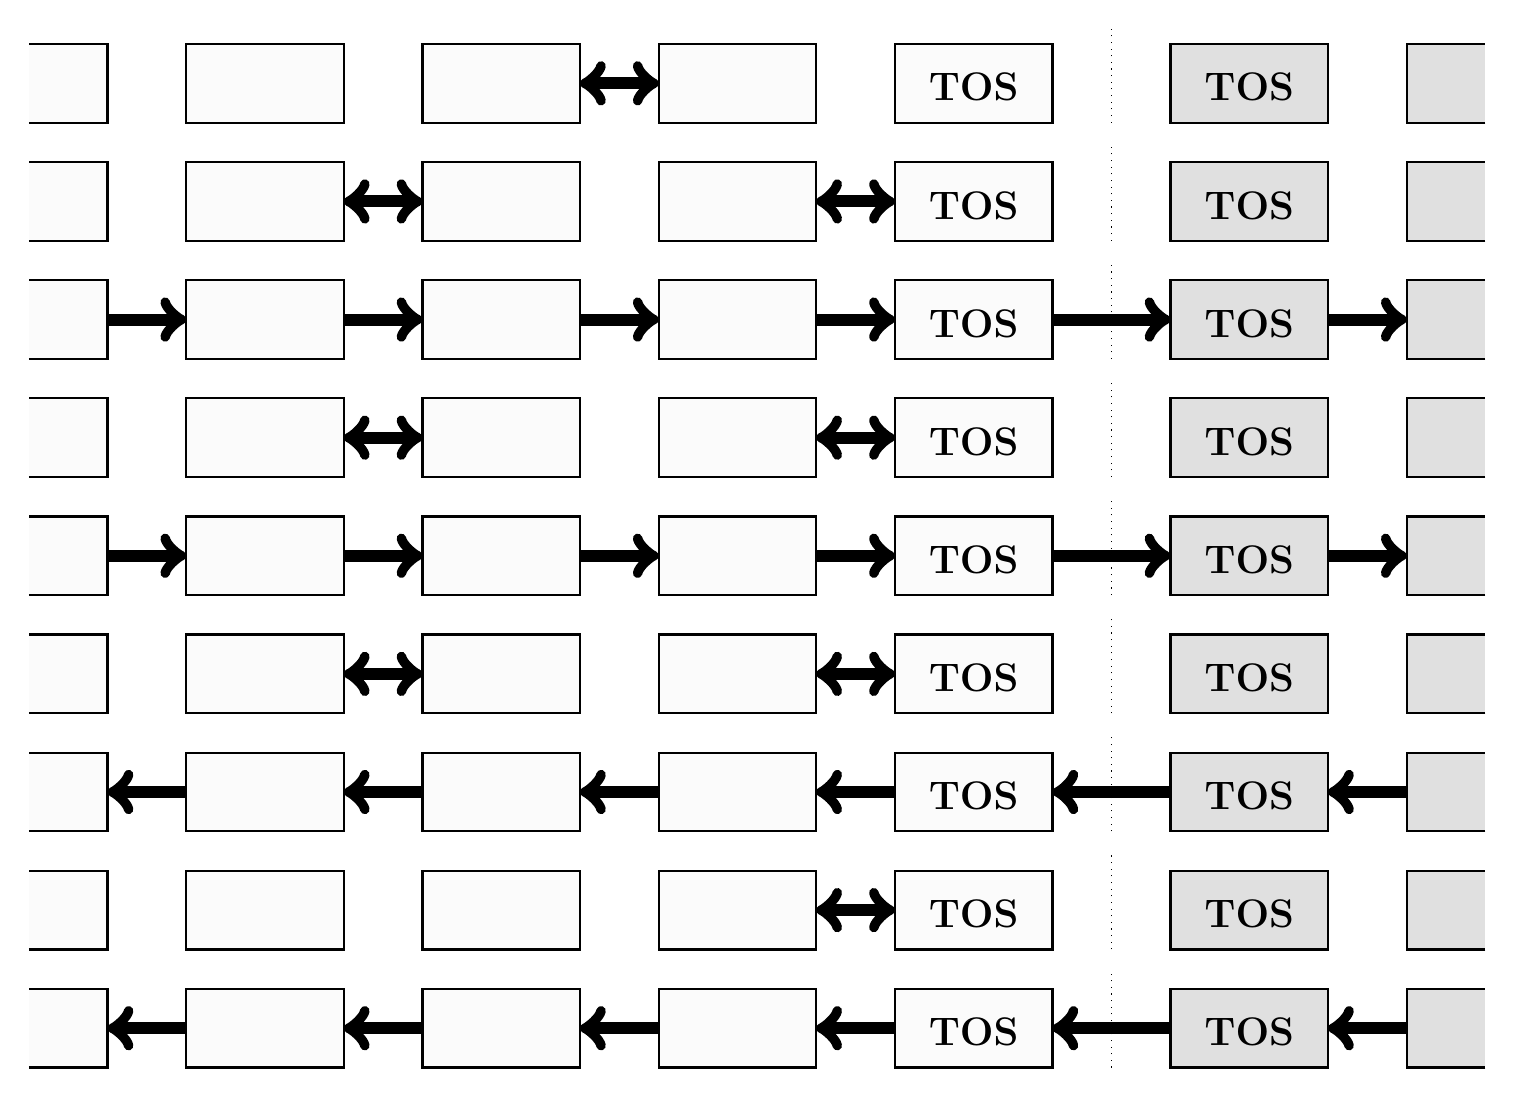
\begin{tikzpicture}
        \draw [thick, fill=gray!3]  (0,12) -- (1,12) -- (1,13) -- (0,13);%
        %\draw [line width=1ex, --] (1,12.5)   -- (2,12.5);          %
        \draw [thick, fill=gray!3]  (2,12) rectangle (4,13);         %PS+3
        %\draw [line width=1ex, --] (4,12.5)   -- (5,12.5);          %
        \draw [thick, fill=gray!3]  (5,12) rectangle (7,13);         %PS+2
        \draw [line width=1ex, <->] (7,12.5)   -- (8,12.5);          %
        \draw [thick, fill=gray!3]  (8,12) rectangle (10,13);        %PS+1
        %\draw [line width=1ex, --] (10,12.5)  -- (11,12.5);         %
        \draw [thick, fill=gray!3]  (11,12) rectangle (13,13);       %PS TOS
        \node at (12,12.45)         {\Large{\textbf{TOS}}};          %
        %\draw [line width=1ex, --] (13,12.5)  -- (14.5,12.5);       %
        \draw [dotted]              (13.75,12) -- (13.75,13.2);      %
        \draw [thick, fill=gray!24] (14.5,12) rectangle (16.5,13);   %RS TOS
        \node at (15.5,12.45)       {\Large{\textbf{TOS}}};          %
        %\draw [line width=1ex, --] (16.5,12.5) -- (17.5,12.5);      % 
        \draw [thick, fill=gray!24] (18.5,12)   -- (17.5,12) -- (17.5,13) -- (18.5,13);

        \draw [thick, fill=gray!3]  (0,10.5) -- (1,10.5) -- (1,11.5) -- (0,11.5);%
        %\draw [line width=1ex, --] (1,11)   -- (2,11);              %
        \draw [thick, fill=gray!3]  (2,10.5) rectangle (4,11.5);     %PS+3
        \draw [line width=1ex, <->] (4,11)   -- (5,11);              %
        \draw [thick, fill=gray!3]  (5,10.5) rectangle (7,11.5);     %PS+2
        %\draw [line width=1ex, --] (7,11)   -- (8,11);              %
        \draw [thick, fill=gray!3]  (8,10.5) rectangle (10,11.5);    %PS+1
        \draw [line width=1ex, <->] (10,11)  -- (11,11);             %
        \draw [thick, fill=gray!3]  (11,10.5) rectangle (13,11.5);   %PS TOS
        \node at (12,10.95)         {\Large{\textbf{TOS}}};          %
        %\draw [line width=1ex, --] (13,11)  -- (14.5,11);           %
        \draw [dotted]              (13.75,10.5) -- (13.75,11.7);    %
        \draw [thick, fill=gray!24] (14.5,10.5) rectangle (16.5,11.5);%RS TOS
        \node at (15.5,10.95)       {\Large{\textbf{TOS}}};          %
        %\draw [line width=1ex, --] (16.5,11) -- (17.5,11);          % 
        \draw [thick, fill=gray!24] (18.5,10.5) -- (17.5,10.5) -- (17.5,11.5) -- (18.5,11.5);

        \draw [thick, fill=gray!3]  (0,9) -- (1,9) -- (1,10) -- (0,10);%
        \draw [line width=1ex, ->]  (1,9.5)   -- (2,9.5);            %
        \draw [thick, fill=gray!3]  (2,9) rectangle (4,10);          %PS+3
        \draw [line width=1ex, ->]  (4,9.5)   -- (5,9.5);            %
        \draw [thick, fill=gray!3]  (5,9) rectangle (7,10);          %PS+2
        \draw [line width=1ex, ->]  (7,9.5)   -- (8,9.5);            %
        \draw [thick, fill=gray!3]  (8,9) rectangle (10,10);         %PS+1
        \draw [line width=1ex, ->]  (10,9.5)  -- (11,9.5);           %
        \draw [thick, fill=gray!3]  (11,9) rectangle (13,10);        %PS TOS
        \node at (12,9.45)          {\Large{\textbf{TOS}}};          %
        \draw [line width=1ex, ->]  (13,9.5)  -- (14.5,9.5);         %
        \draw [dotted]              (13.75,9) -- (13.75,10.2);       %
        \draw [thick, fill=gray!24] (14.5,9) rectangle (16.5,10);    %RS TOS
        \node at (15.5,9.45)        {\Large{\textbf{TOS}}};          %
        \draw [line width=1ex, ->]  (16.5,9.5) -- (17.5,9.5);        % 
        \draw [thick, fill=gray!24] (18.5,9)   -- (17.5,9) -- (17.5,10) -- (18.5,10);

        \draw [thick, fill=gray!3]  (0,7.5) -- (1,7.5) -- (1,8.5) -- (0,8.5);%
        %\draw [line width=1ex, --] (1,8)   -- (2,8);                %
        \draw [thick, fill=gray!3]  (2,7.5) rectangle (4,8.5);       %PS+3
        \draw [line width=1ex, <->] (4,8)   -- (5,8);                %
        \draw [thick, fill=gray!3]  (5,7.5) rectangle (7,8.5);       %PS+2
        %\draw [line width=1ex, --] (7,8)   -- (8,8);                %
        \draw [thick, fill=gray!3]  (8,7.5) rectangle (10,8.5);      %PS+1
        \draw [line width=1ex, <->] (10,8)  -- (11,8);               %
        \draw [thick, fill=gray!3]  (11,7.5) rectangle (13,8.5);     %PS TOS
        \node at (12,7.95)          {\Large{\textbf{TOS}}};          %
        %\draw [line width=1ex, --] (13,8)  -- (14.5,8);             %
        \draw [dotted]              (13.75,7.5) -- (13.75,8.7);      %
        \draw [thick, fill=gray!24] (14.5,7.5) rectangle (16.5,8.5); %RS TOS
        \node at (15.5,7.95)        {\Large{\textbf{TOS}}};          %
        %\draw [line width=1ex, --] (16.5,8) -- (17.5,8);            % 
        \draw [thick, fill=gray!24] (18.5,7.5) -- (17.5,7.5) -- (17.5,8.5) -- (18.5,8.5);

        \draw [thick, fill=gray!3]  (0,6) -- (1,6) -- (1,7) -- (0,7);%
        \draw [line width=1ex, ->] (1,6.5)   -- (2,6.5);             %
        \draw [thick, fill=gray!3]  (2,6) rectangle (4,7);           %PS+3
        \draw [line width=1ex, ->] (4,6.5)   -- (5,6.5);             %
        \draw [thick, fill=gray!3]  (5,6) rectangle (7,7);           %PS+2
        \draw [line width=1ex, ->] (7,6.5)   -- (8,6.5);             %
        \draw [thick, fill=gray!3]  (8,6) rectangle (10,7);          %PS+1
        \draw [line width=1ex, ->] (10,6.5)  -- (11,6.5);            %
        \draw [thick, fill=gray!3]  (11,6) rectangle (13,7);         %PS TOS
        \node at (12,6.45)          {\Large{\textbf{TOS}}};          %
        \draw [line width=1ex, ->] (13,6.5)  -- (14.5,6.5);          %
        \draw [dotted]              (13.75,6) -- (13.75,7.2);        %
        \draw [thick, fill=gray!24] (14.5,6) rectangle (16.5,7);     %RS TOS
        \node at (15.5,6.45)        {\Large{\textbf{TOS}}};          %
        \draw [line width=1ex, ->]  (16.5,6.5) -- (17.5,6.5);        % 
        \draw [thick, fill=gray!24] (18.5,6)   -- (17.5,6) -- (17.5,7) -- (18.5,7);

        \draw [thick, fill=gray!3]  (0,4.5) -- (1,4.5) -- (1,5.5) -- (0,5.5);%
        %\draw [line width=1ex, --] (1,5)   -- (2,5);                %
        \draw [thick, fill=gray!3]  (2,4.5) rectangle (4,5.5);       %PS+3
        \draw [line width=1ex, <->] (4,5)   -- (5,5);                %
        \draw [thick, fill=gray!3]  (5,4.5) rectangle (7,5.5);       %PS+2
        %\draw [line width=1ex, --] (7,5)   -- (8,5);                %
        \draw [thick, fill=gray!3]  (8,4.5) rectangle (10,5.5);      %PS+1
        \draw [line width=1ex, <->] (10,5)  -- (11,5);               %
        \draw [thick, fill=gray!3]  (11,4.5) rectangle (13,5.5);     %PS TOS
        \node at (12,4.95)          {\Large{\textbf{TOS}}};          %
        %\draw [line width=1ex, --] (13,5)  -- (14.5,5);             %
        \draw [dotted]              (13.75,4.5) -- (13.75,5.7);      %
        \draw [thick, fill=gray!24] (14.5,4.5) rectangle (16.5,5.5); %RS TOS
        \node at (15.5,4.95)        {\Large{\textbf{TOS}}};          %
        %\draw [line width=1ex, --] (16.5,5) -- (17.5,5);            % 
        \draw [thick, fill=gray!24] (18.5,4.5) -- (17.5,4.5) -- (17.5,5.5) -- (18.5,5.5);

        \draw [thick, fill=gray!3]  (0,3) -- (1,3) -- (1,4) -- (0,4);%
        \draw [line width=1ex, <-]  (1,3.5)   -- (2,3.5);            %
        \draw [thick, fill=gray!3]  (2,3) rectangle (4,4);           %PS+3
        \draw [line width=1ex, <-]  (4,3.5)   -- (5,3.5);            %
        \draw [thick, fill=gray!3]  (5,3) rectangle (7,4);           %PS+2
        \draw [line width=1ex, <-]  (7,3.5)   -- (8,3.5);            %
        \draw [thick, fill=gray!3]  (8,3) rectangle (10,4);          %PS+1
        \draw [line width=1ex, <-]  (10,3.5)  -- (11,3.5);           %
        \draw [thick, fill=gray!3]  (11,3) rectangle (13,4);         %PS TOS
        \node at (12,3.45)          {\Large{\textbf{TOS}}};          %
        \draw [line width=1ex, <-]  (13,3.5)  -- (14.5,3.5);         %
        \draw [dotted]              (13.75,3) -- (13.75,4.2);        %
        \draw [thick, fill=gray!24] (14.5,3) rectangle (16.5,4);     %RS TOS
        \node at (15.5,3.45)        {\Large{\textbf{TOS}}};          %
        \draw [line width=1ex, <-]  (16.5,3.5) -- (17.5,3.5);        % 
        \draw [thick, fill=gray!24] (18.5,3)   -- (17.5,3) -- (17.5,4) -- (18.5,4);

        \draw [thick, fill=gray!3]  (0,1.5) -- (1,1.5) -- (1,2.5) -- (0,2.5);%
        %\draw [line width=1ex, --] (1,2)   -- (2,2);                %
        \draw [thick, fill=gray!3]  (2,1.5) rectangle (4,2.5);       %PS+3
        %\draw [line width=1ex, --] (4,2)   -- (5,2);                %
        \draw [thick, fill=gray!3]  (5,1.5) rectangle (7,2.5);       %PS+2
        %\draw [line width=1ex, --] (7,2)   -- (8,2);                %
        \draw [thick, fill=gray!3]  (8,1.5) rectangle (10,2.5);      %PS+1
        \draw [line width=1ex, <->] (10,2)  -- (11,2);               %
        \draw [thick, fill=gray!3]  (11,1.5) rectangle (13,2.5);     %PS TOS
        \node at (12,1.95)          {\Large{\textbf{TOS}}};          %
        %\draw [line width=1ex, --] (13,2)  -- (14.5,2);             %
        \draw [dotted]              (13.75,1.5) -- (13.75,2.7);      %
        \draw [thick, fill=gray!24] (14.5,1.5) rectangle (16.5,2.5); %RS TOS
        \node at (15.5,1.95)        {\Large{\textbf{TOS}}};          %
        %\draw [line width=1ex, --] (16.5,2) -- (17.5,2);            % 
        \draw [thick, fill=gray!24] (18.5,1.5) -- (17.5,1.5) -- (17.5,2.5) -- (18.5,2.5);

        \draw [thick, fill=gray!3]  (0,0) -- (1,0) -- (1,1) -- (0,1);%
        \draw [line width=1ex, <-] (1,0.5) -- (2,0.5);               %
        \draw [thick, fill=gray!3]  (2,0) rectangle (4,1);           %PS+3
        \draw [line width=1ex, <-] (4,0.5) -- (5,0.5);               %
        \draw [thick, fill=gray!3]  (5,0) rectangle (7,1);           %PS+2
        \draw [line width=1ex, <-] (7,0.5) -- (8,0.5);               %
        \draw [thick, fill=gray!3]  (8,0) rectangle (10,1);          %PS+1
        \draw [line width=1ex, <-] (10,0.5) -- (11,0.5);             %
        \draw [thick, fill=gray!3]  (11,0) rectangle (13,1);         %PS TOS
        \node at (12,0.45)          {\Large{\textbf{TOS}}};          %
        \draw [line width=1ex, <-] (13,0.5)  -- (14.5,0.5);          %
        \draw [dotted]              (13.75,0) -- (13.75,1.2);        %
        \draw [thick, fill=gray!24] (14.5,0) rectangle (16.5,1);     %RS TOS
        \node at (15.5,0.45)        {\Large{\textbf{TOS}}};          %
        \draw [line width=1ex, <-] (16.5,0.5) -- (17.5,0.5);         % 
        \draw [thick, fill=gray!24] (18.5,0) -- (17.5,0) -- (17.5,1) -- (18.5,1);
      \end{tikzpicture}
    }} &
    \multicolumn{1}{m{4.25em}|}{
    \makecell[c]{ 
      \texttt{0x0460} \\ 
      \texttt{0x0598} \\ 
      \texttt{0x06AB} \\ 
      \texttt{0x0598} \\ 
      \texttt{0x06AB} \\ 
      \texttt{0x0598} \\ 
      \texttt{0x0755} \\ 
      \texttt{0x0418} \\ 
      \texttt{0x0755}
    }} \\ \hline

    %2RDROP
    \texttt{2RDROP} &
      ( R: x1 x2 -- ) &
    \multicolumn{1}{m{21.35em}|}{
    \scalebox{0.4} {
      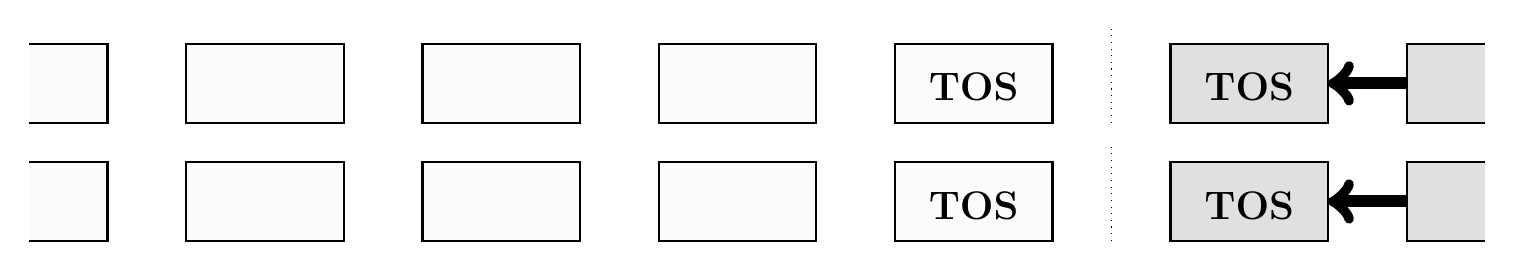
\begin{tikzpicture}
        \draw [thick, fill=gray!3]  (0,1.5) -- (1,1.5) -- (1,2.5) -- (0,2.5);%
        %\draw [line width=1ex, --] (1,2)   -- (2,2);                %
        \draw [thick, fill=gray!3]  (2,1.5) rectangle (4,2.5);       %PS+3
        %\draw [line width=1ex, --] (4,2)   -- (5,2);                %
        \draw [thick, fill=gray!3]  (5,1.5) rectangle (7,2.5);       %PS+2
        %\draw [line width=1ex, --] (7,2)   -- (8,2);                %
        \draw [thick, fill=gray!3]  (8,1.5) rectangle (10,2.5);      %PS+1
        %\draw [line width=1ex, --] (10,2)  -- (11,2);               %
        \draw [thick, fill=gray!3]  (11,1.5) rectangle (13,2.5);     %PS TOS
        \node at (12,1.95)          {\Large{\textbf{TOS}}};          %
        %\draw [line width=1ex, --] (13,2)  -- (14.5,2);             %
        \draw [dotted]              (13.75,1.5) -- (13.75,2.7);      %
        \draw [thick, fill=gray!24] (14.5,1.5) rectangle (16.5,2.5); %RS TOS
        \node at (15.5,1.95)        {\Large{\textbf{TOS}}};          %
        \draw [line width=1ex, <-]  (16.5,2) -- (17.5,2);            % 
        \draw [thick, fill=gray!24] (18.5,1.5) -- (17.5,1.5) -- (17.5,2.5) -- (18.5,2.5);

        \draw [thick, fill=gray!3]  (0,0) -- (1,0) -- (1,1) -- (0,1);%
        %\draw [line width=1ex, --] (1,0.5) -- (2,0.5);              %
        \draw [thick, fill=gray!3]  (2,0) rectangle (4,1);           %PS+3
        %\draw [line width=1ex, --] (4,0.5) -- (5,0.5);              %
        \draw [thick, fill=gray!3]  (5,0) rectangle (7,1);           %PS+2
        %\draw [line width=1ex, --] (7,0.5) -- (8,0.5);              %
        \draw [thick, fill=gray!3]  (8,0) rectangle (10,1);          %PS+1
        %\draw [line width=1ex, --] (10,0.5) -- (11,0.5);            %
        \draw [thick, fill=gray!3]  (11,0) rectangle (13,1);         %PS TOS
        \node at (12,0.45)          {\Large{\textbf{TOS}}};          %
        %\draw [line width=1ex, --] (13,0.5)  -- (14.5,0.5);         %
        \draw [dotted]              (13.75,0) -- (13.75,1.2);        %
        \draw [thick, fill=gray!24] (14.5,0) rectangle (16.5,1);     %RS TOS
        \node at (15.5,0.45)        {\Large{\textbf{TOS}}};          %
        \draw [line width=1ex, <-]  (16.5,0.5) -- (17.5,0.5);        % 
        \draw [thick, fill=gray!24] (18.5,0) -- (17.5,0) -- (17.5,1) -- (18.5,1);
      \end{tikzpicture}
    }} &
    \multicolumn{1}{m{4.25em}|}{
    \makecell[c]{ 
      \texttt{0x0401} \\ 
      \texttt{0x0401}
    }} \\ \hline

    %2RDUP
    \texttt{2RDUP} &
    ( R: x1 x2 -- x1 x2 x1 x2 ) &
    \multicolumn{1}{m{21.35em}|}{
    \scalebox{0.4} {
      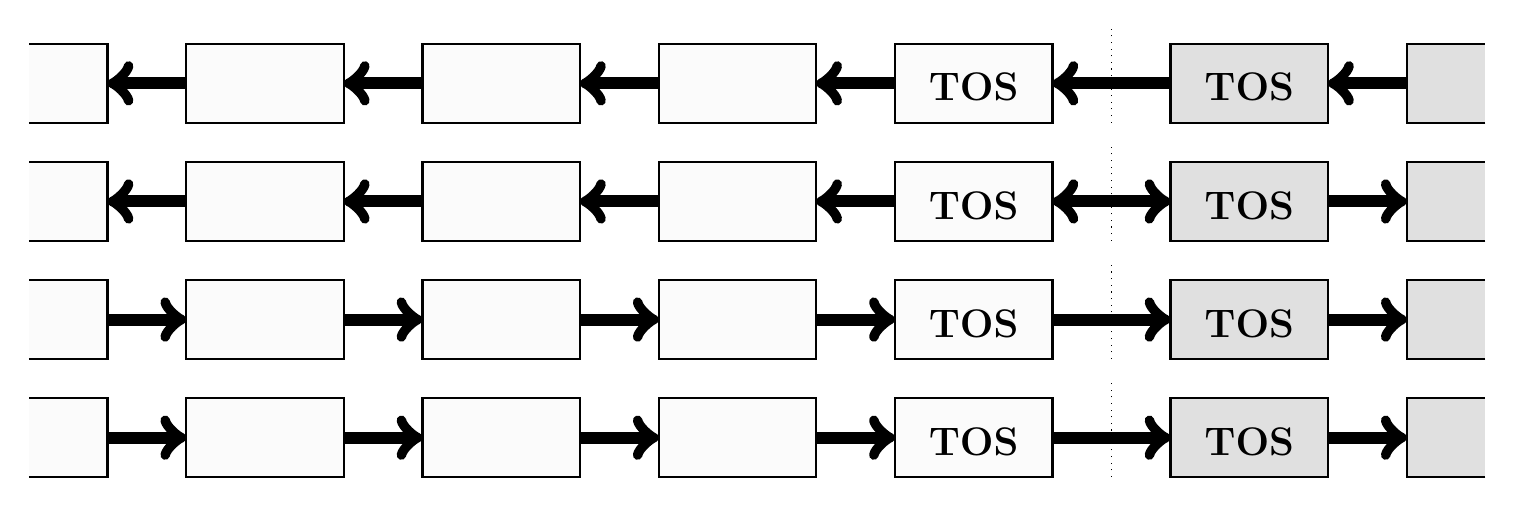
\begin{tikzpicture}
        \draw [thick, fill=gray!3]  (0,4.5) -- (1,4.5) -- (1,5.5) -- (0,5.5);%
        \draw [line width=1ex, <-]  (1,5)   -- (2,5);                %
        \draw [thick, fill=gray!3]  (2,4.5) rectangle (4,5.5);       %PS+3
        \draw [line width=1ex, <-]  (4,5)   -- (5,5);                %
        \draw [thick, fill=gray!3]  (5,4.5) rectangle (7,5.5);       %PS+2
        \draw [line width=1ex, <-]  (7,5)   -- (8,5);                %
        \draw [thick, fill=gray!3]  (8,4.5) rectangle (10,5.5);      %PS+1
        \draw [line width=1ex, <-]  (10,5)  -- (11,5);               %
        \draw [thick, fill=gray!3]  (11,4.5) rectangle (13,5.5);     %PS TOS
        \node at (12,4.95)          {\Large{\textbf{TOS}}};          %
        \draw [line width=1ex, <-]  (13,5)  -- (14.5,5);             %
        \draw [dotted]              (13.75,4.5) -- (13.75,5.7);      %
        \draw [thick, fill=gray!24] (14.5,4.5) rectangle (16.5,5.5); %RS TOS
        \node at (15.5,4.95)        {\Large{\textbf{TOS}}};          %
        \draw [line width=1ex, <-]  (16.5,5) -- (17.5,5);            % 
        \draw [thick, fill=gray!24] (18.5,4.5) -- (17.5,4.5) -- (17.5,5.5) -- (18.5,5.5);

        \draw [thick, fill=gray!3]  (0,3) -- (1,3) -- (1,4) -- (0,4);%
        \draw [line width=1ex, <-]  (1,3.5)   -- (2,3.5);            %
        \draw [thick, fill=gray!3]  (2,3) rectangle (4,4);           %PS+3
        \draw [line width=1ex, <-]  (4,3.5)   -- (5,3.5);            %
        \draw [thick, fill=gray!3]  (5,3) rectangle (7,4);           %PS+2
        \draw [line width=1ex, <-]  (7,3.5)   -- (8,3.5);            %
        \draw [thick, fill=gray!3]  (8,3) rectangle (10,4);          %PS+1
        \draw [line width=1ex, <-]  (10,3.5)  -- (11,3.5);           %
        \draw [thick, fill=gray!3]  (11,3) rectangle (13,4);         %PS TOS
        \node at (12,3.45)          {\Large{\textbf{TOS}}};          %
        \draw [line width=1ex, <->] (13,3.5)  -- (14.5,3.5);         %
        \draw [dotted]              (13.75,3) -- (13.75,4.2);        %
        \draw [thick, fill=gray!24] (14.5,3) rectangle (16.5,4);     %RS TOS
        \node at (15.5,3.45)        {\Large{\textbf{TOS}}};          %
        \draw [line width=1ex, ->]  (16.5,3.5) -- (17.5,3.5);        % 
        \draw [thick, fill=gray!24] (18.5,3)   -- (17.5,3) -- (17.5,4) -- (18.5,4);

        \draw [thick, fill=gray!3]  (0,1.5) -- (1,1.5) -- (1,2.5) -- (0,2.5);%
        \draw [line width=1ex, ->]  (1,2)   -- (2,2);                %
        \draw [thick, fill=gray!3]  (2,1.5) rectangle (4,2.5);       %PS+3
        \draw [line width=1ex, ->]  (4,2)   -- (5,2);                %
        \draw [thick, fill=gray!3]  (5,1.5) rectangle (7,2.5);       %PS+2
        \draw [line width=1ex, ->]  (7,2)   -- (8,2);                %
        \draw [thick, fill=gray!3]  (8,1.5) rectangle (10,2.5);      %PS+1
        \draw [line width=1ex, ->]  (10,2)  -- (11,2);               %
        \draw [thick, fill=gray!3]  (11,1.5) rectangle (13,2.5);     %PS TOS
        \node at (12,1.95)          {\Large{\textbf{TOS}}};          %
        \draw [line width=1ex, ->]  (13,2)  -- (14.5,2);             %
        \draw [dotted]              (13.75,1.5) -- (13.75,2.7);      %
        \draw [thick, fill=gray!24] (14.5,1.5) rectangle (16.5,2.5); %RS TOS
        \node at (15.5,1.95)        {\Large{\textbf{TOS}}};          %
        \draw [line width=1ex, ->]  (16.5,2) -- (17.5,2);            % 
        \draw [thick, fill=gray!24] (18.5,1.5) -- (17.5,1.5) -- (17.5,2.5) -- (18.5,2.5);

        \draw [thick, fill=gray!3]  (0,0) -- (1,0) -- (1,1) -- (0,1);%
        \draw [line width=1ex, ->]  (1,0.5) -- (2,0.5);              %
        \draw [thick, fill=gray!3]  (2,0) rectangle (4,1);           %PS+3
        \draw [line width=1ex, ->]  (4,0.5) -- (5,0.5);              %
        \draw [thick, fill=gray!3]  (5,0) rectangle (7,1);           %PS+2
        \draw [line width=1ex, ->]  (7,0.5) -- (8,0.5);              %
        \draw [thick, fill=gray!3]  (8,0) rectangle (10,1);          %PS+1
        \draw [line width=1ex, ->]  (10,0.5) -- (11,0.5);            %
        \draw [thick, fill=gray!3]  (11,0) rectangle (13,1);         %PS TOS
        \node at (12,0.45)          {\Large{\textbf{TOS}}};          %
        \draw [line width=1ex, ->]  (13,0.5)  -- (14.5,0.5);         %
        \draw [dotted]              (13.75,0) -- (13.75,1.2);        %
        \draw [thick, fill=gray!24] (14.5,0) rectangle (16.5,1);     %RS TOS
        \node at (15.5,0.45)        {\Large{\textbf{TOS}}};          %
        \draw [line width=1ex, ->]  (16.5,0.5) -- (17.5,0.5);        % 
        \draw [thick, fill=gray!24] (18.5,0) -- (17.5,0) -- (17.5,1) -- (18.5,1);
      \end{tikzpicture}
    }} &
    \multicolumn{1}{m{4.25em}|}{
    \makecell[c]{ 
      \texttt{0x0755} \\ 
      \texttt{0x0757} \\ 
      \texttt{0x06AB} \\ 
      \texttt{0x06AB}
    }} \\ \hline

    %2>R
    \texttt{2>R} &
    \multicolumn{1}{m{18.3em}|}{
    \makecell[c]{ 
      ( x1 x2 -- )\\
      ( R: -- x1 x2 )
    }} &
    \multicolumn{1}{m{21.35em}|}{
    \scalebox{0.4} {
      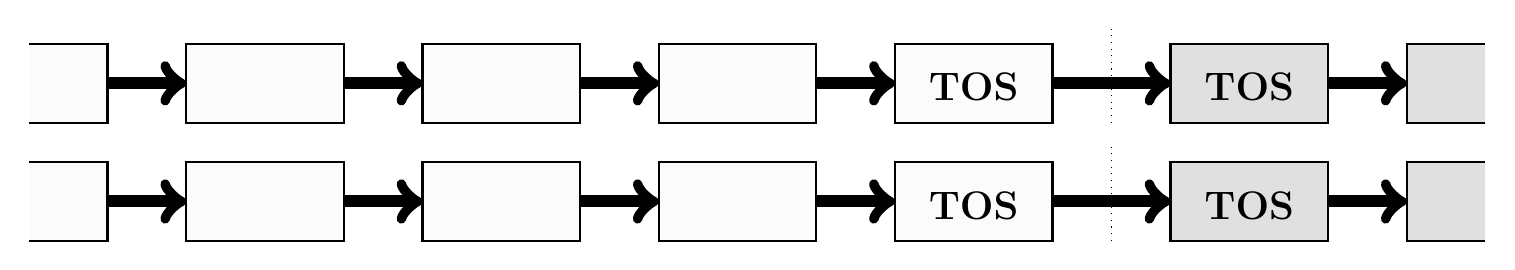
\begin{tikzpicture}
        \draw [thick, fill=gray!3]  (0,1.5) -- (1,1.5) -- (1,2.5) -- (0,2.5);%
        \draw [line width=1ex, ->]  (1,2)   -- (2,2);                %
        \draw [thick, fill=gray!3]  (2,1.5) rectangle (4,2.5);       %PS+3
        \draw [line width=1ex, ->]  (4,2)   -- (5,2);                %
        \draw [thick, fill=gray!3]  (5,1.5) rectangle (7,2.5);       %PS+2
        \draw [line width=1ex, ->]  (7,2)   -- (8,2);                %
        \draw [thick, fill=gray!3]  (8,1.5) rectangle (10,2.5);      %PS+1
        \draw [line width=1ex, ->]  (10,2)  -- (11,2);               %
        \draw [thick, fill=gray!3]  (11,1.5) rectangle (13,2.5);     %PS TOS
        \node at (12,1.95)          {\Large{\textbf{TOS}}};          %
        \draw [line width=1ex, ->]  (13,2)  -- (14.5,2);             %
        \draw [dotted]              (13.75,1.5) -- (13.75,2.7);      %
        \draw [thick, fill=gray!24] (14.5,1.5) rectangle (16.5,2.5); %RS TOS
        \node at (15.5,1.95)        {\Large{\textbf{TOS}}};          %
        \draw [line width=1ex, ->]  (16.5,2) -- (17.5,2);            % 
        \draw [thick, fill=gray!24] (18.5,1.5) -- (17.5,1.5) -- (17.5,2.5) -- (18.5,2.5);

        \draw [thick, fill=gray!3]  (0,0) -- (1,0) -- (1,1) -- (0,1);%
        \draw [line width=1ex, ->]  (1,0.5) -- (2,0.5);              %
        \draw [thick, fill=gray!3]  (2,0) rectangle (4,1);           %PS+3
        \draw [line width=1ex, ->]  (4,0.5) -- (5,0.5);              %
        \draw [thick, fill=gray!3]  (5,0) rectangle (7,1);           %PS+2
        \draw [line width=1ex, ->]  (7,0.5) -- (8,0.5);              %
        \draw [thick, fill=gray!3]  (8,0) rectangle (10,1);          %PS+1
        \draw [line width=1ex, ->]  (10,0.5) -- (11,0.5);            %
        \draw [thick, fill=gray!3]  (11,0) rectangle (13,1);         %PS TOS
        \node at (12,0.45)          {\Large{\textbf{TOS}}};          %
        \draw [line width=1ex, ->]  (13,0.5)  -- (14.5,0.5);         %
        \draw [dotted]              (13.75,0) -- (13.75,1.2);        %
        \draw [thick, fill=gray!24] (14.5,0) rectangle (16.5,1);     %RS TOS
        \node at (15.5,0.45)        {\Large{\textbf{TOS}}};          %
        \draw [line width=1ex, ->]  (16.5,0.5) -- (17.5,0.5);        % 
        \draw [thick, fill=gray!24] (18.5,0) -- (17.5,0) -- (17.5,1) -- (18.5,1);
      \end{tikzpicture}
    }} &
    \multicolumn{1}{m{4.25em}|}{
    \makecell[c]{ 
      \texttt{0x06AB} \\ 
      \texttt{0x06AB}
    }} \\ \hline

    %2R@
    \texttt{2R@} &
    \multicolumn{1}{m{18.3em}|}{
    \makecell[c]{ 
      ( -- x1 x2 )\\
      ( R: x1 x2 -- x1 x2 )
    }} &
    \multicolumn{1}{m{21.35em}|}{
    \scalebox{0.4} {
      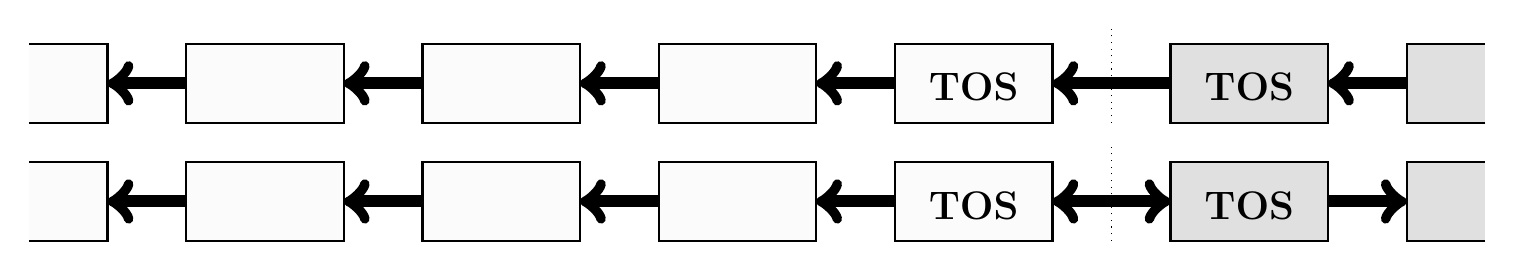
\begin{tikzpicture}
        \draw [thick, fill=gray!3]  (0,1.5) -- (1,1.5) -- (1,2.5) -- (0,2.5);%
        \draw [line width=1ex, <-]  (1,2)   -- (2,2);                %
        \draw [thick, fill=gray!3]  (2,1.5) rectangle (4,2.5);       %PS+3
        \draw [line width=1ex, <-]  (4,2)   -- (5,2);                %
        \draw [thick, fill=gray!3]  (5,1.5) rectangle (7,2.5);       %PS+2
        \draw [line width=1ex, <-]  (7,2)   -- (8,2);                %
        \draw [thick, fill=gray!3]  (8,1.5) rectangle (10,2.5);      %PS+1
        \draw [line width=1ex, <-]  (10,2)  -- (11,2);               %
        \draw [thick, fill=gray!3]  (11,1.5) rectangle (13,2.5);     %PS TOS
        \node at (12,1.95)          {\Large{\textbf{TOS}}};          %
        \draw [line width=1ex, <-]  (13,2)  -- (14.5,2);             %
        \draw [dotted]              (13.75,1.5) -- (13.75,2.7);      %
        \draw [thick, fill=gray!24] (14.5,1.5) rectangle (16.5,2.5); %RS TOS
        \node at (15.5,1.95)        {\Large{\textbf{TOS}}};          %
        \draw [line width=1ex, <-]  (16.5,2) -- (17.5,2);            % 
        \draw [thick, fill=gray!24] (18.5,1.5) -- (17.5,1.5) -- (17.5,2.5) -- (18.5,2.5);

        \draw [thick, fill=gray!3]  (0,0) -- (1,0) -- (1,1) -- (0,1);%
        \draw [line width=1ex, <-]  (1,0.5) -- (2,0.5);              %
        \draw [thick, fill=gray!3]  (2,0) rectangle (4,1);           %PS+3
        \draw [line width=1ex, <-]  (4,0.5) -- (5,0.5);              %
        \draw [thick, fill=gray!3]  (5,0) rectangle (7,1);           %PS+2
        \draw [line width=1ex, <-]  (7,0.5) -- (8,0.5);              %
        \draw [thick, fill=gray!3]  (8,0) rectangle (10,1);          %PS+1
        \draw [line width=1ex, <-]  (10,0.5) -- (11,0.5);            %
        \draw [thick, fill=gray!3]  (11,0) rectangle (13,1);         %PS TOS
        \node at (12,0.45)          {\Large{\textbf{TOS}}};          %
        \draw [line width=1ex, <->] (13,0.5)  -- (14.5,0.5);         %
        \draw [dotted]              (13.75,0) -- (13.75,1.2);        %
        \draw [thick, fill=gray!24] (14.5,0) rectangle (16.5,1);     %RS TOS
        \node at (15.5,0.45)        {\Large{\textbf{TOS}}};          %
        \draw [line width=1ex, ->]  (16.5,0.5) -- (17.5,0.5);        % 
        \draw [thick, fill=gray!24] (18.5,0) -- (17.5,0) -- (17.5,1) -- (18.5,1);
      \end{tikzpicture}
    }} &
    \multicolumn{1}{m{4.25em}|}{
    \makecell[c]{ 
      \texttt{0x0755} \\ 
      \texttt{0x0757}
    }} \\ \hline

    %2R>
    \texttt{2R>} &
    \multicolumn{1}{m{18.3em}|}{
    \makecell[c]{ 
      ( -- x1 x2 )\\
      ( R: x1 x2 -- )
    }} &
    \multicolumn{1}{m{21.35em}|}{
    \scalebox{0.4} {
      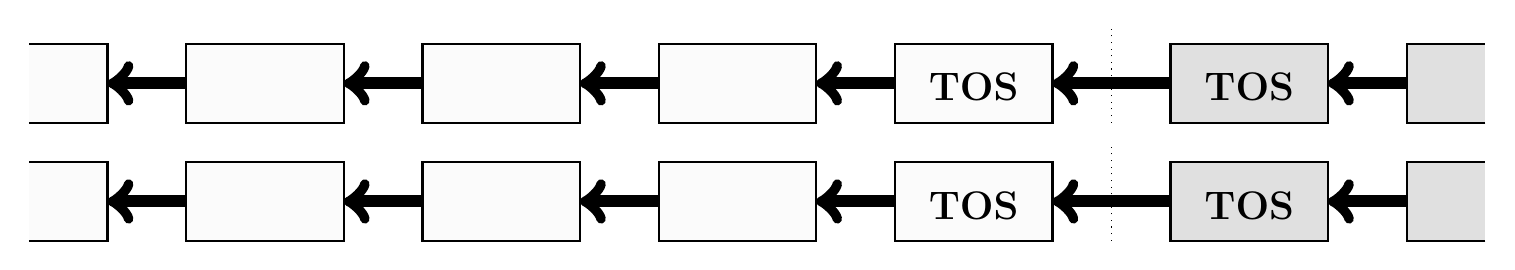
\begin{tikzpicture}

        \draw [thick, fill=gray!3]  (0,1.5) -- (1,1.5) -- (1,2.5) -- (0,2.5);%
        \draw [line width=1ex, <-]  (1,2)   -- (2,2);                %
        \draw [thick, fill=gray!3]  (2,1.5) rectangle (4,2.5);       %PS+3
        \draw [line width=1ex, <-]  (4,2)   -- (5,2);                %
        \draw [thick, fill=gray!3]  (5,1.5) rectangle (7,2.5);       %PS+2
        \draw [line width=1ex, <-]  (7,2)   -- (8,2);                %
        \draw [thick, fill=gray!3]  (8,1.5) rectangle (10,2.5);      %PS+1
        \draw [line width=1ex, <-]  (10,2)  -- (11,2);               %
        \draw [thick, fill=gray!3]  (11,1.5) rectangle (13,2.5);     %PS TOS
        \node at (12,1.95)          {\Large{\textbf{TOS}}};          %
        \draw [line width=1ex, <-]  (13,2)  -- (14.5,2);             %
        \draw [dotted]              (13.75,1.5) -- (13.75,2.7);      %
        \draw [thick, fill=gray!24] (14.5,1.5) rectangle (16.5,2.5); %RS TOS
        \node at (15.5,1.95)        {\Large{\textbf{TOS}}};          %
        \draw [line width=1ex, <-]  (16.5,2) -- (17.5,2);            % 
        \draw [thick, fill=gray!24] (18.5,1.5) -- (17.5,1.5) -- (17.5,2.5) -- (18.5,2.5);

        \draw [thick, fill=gray!3]  (0,0) -- (1,0) -- (1,1) -- (0,1);%
        \draw [line width=1ex, <-]  (1,0.5) -- (2,0.5);              %
        \draw [thick, fill=gray!3]  (2,0) rectangle (4,1);           %PS+3
        \draw [line width=1ex, <-]  (4,0.5) -- (5,0.5);              %
        \draw [thick, fill=gray!3]  (5,0) rectangle (7,1);           %PS+2
        \draw [line width=1ex, <-]  (7,0.5) -- (8,0.5);              %
        \draw [thick, fill=gray!3]  (8,0) rectangle (10,1);          %PS+1
        \draw [line width=1ex, <-]  (10,0.5) -- (11,0.5);            %
        \draw [thick, fill=gray!3]  (11,0) rectangle (13,1);         %PS TOS
        \node at (12,0.45)          {\Large{\textbf{TOS}}};          %
        \draw [line width=1ex, <-]  (13,0.5)  -- (14.5,0.5);         %
        \draw [dotted]              (13.75,0) -- (13.75,1.2);        %
        \draw [thick, fill=gray!24] (14.5,0) rectangle (16.5,1);     %RS TOS
        \node at (15.5,0.45)        {\Large{\textbf{TOS}}};          %
        \draw [line width=1ex, <-]  (16.5,0.5) -- (17.5,0.5);        % 
        \draw [thick, fill=gray!24] (18.5,0) -- (17.5,0) -- (17.5,1) -- (18.5,1);
      \end{tikzpicture}
    }} &
    \multicolumn{1}{m{4.25em}|}{
    \makecell[c]{ 
      \texttt{0x0755} \\ 
      \texttt{0x0755}
    }} \\ \hline
  \end{longtable}
\end{center}  
\endgroup

\subsubsection{Stack Underflow Detection}
\label{opcodes:stack:uf}

The required number of arguments for a stack instruction is determined by the transition pattern
(\gls{ust} and \gls{ist} fields).
The rules listed in \tabref{opcodes:stack:ufrules} are applied.


subsubsection{Common Stack Operations}
\label{opcodes:stack:ops}
\tabref{opcodes:stack:mapping} shows how common \gls{stack} operations in \gls{forth} are mapped N1 instructions. 

\begingroup
\setlength{\LTleft}{-20cm plus -1fill}
\setlength{\LTright}{\LTleft}
\begin{center}
  \rowcolors{1}{gray!12}{white}                                         %set alternating row color
  \begin{longtable}{|c|c|c|}
    \rowcolor{white}
    \caption{Rules of Stack Underflow Detection}
    \label{opcodes:stack:ufrules} \\
    %Header
    \hline                                     
    \rowcolor{gray!25}
    \multicolumn{1}{|c|}{\textbf{\rule{0pt}{2.5ex}Rule}}       &  
    \multicolumn{1}{c|}{\textbf{\rule{0pt}{2.5ex}Transitions}} & 
    \multicolumn{1}{c|}{\textbf{\rule{0pt}{2.5ex}Description}} \\
    \hline
    \endhead                               
    %Footers
    \hline
    \rowcolor{white}
    \multicolumn{3}{r}{\tiny{...continued}} \\
    \endfoot
    \hline
    \endlastfoot

    %DROP rule
    \multicolumn{1}{|m{3em}|}{
    \makecell[c]{ 
      ``\texttt{DROP}''\\
      Rule}} &
    \multicolumn{1}{m{7em}|}{
    \scalebox{0.4} {
      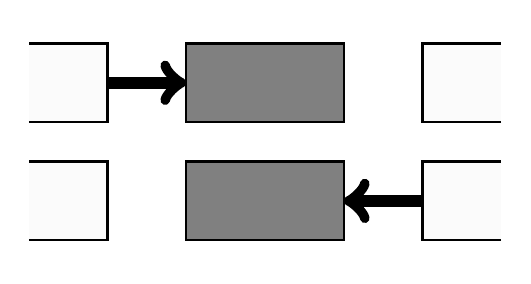
\begin{tikzpicture}
        \path []  (0,-0.2)   -- (0,2.7);       
        
        \draw [thick, fill=gray!3]  (0,1.5) -- (1,1.5) -- (1,2.5) -- (0,2.5);
        \draw [line width=1ex, ->]  (1,2)   -- (2,2);                        
        \draw [thick, fill=gray]    (2,1.5) rectangle (4,2.5);              
        \draw [thick, fill=gray!3]  (6,1.5) -- (5,1.5) -- (5,2.5) -- (6,2.5);

        \draw [thick, fill=gray!3]  (0,0) -- (1,0) -- (1,1) -- (0,1);        
        \draw [thick, fill=gray]    (2,0) rectangle (4,1);                   
        \draw [line width=1ex, <-]  (4,0.5) -- (5,0.5);                      
        \draw [thick, fill=gray!3]  (6,0) -- (5,0) -- (5,1) -- (6,1);
      \end{tikzpicture}
    }} &
    %\multicolumn{1}{m{32em}|}{
    \makecell[l]{
    \begin{minipage}[t]{\linewidth}%  
      A cell that will be dropped (overwritten, without passing on it's content)
      from either direction must hold content, otherwise a stack underflow exception
      will be triggered.
    \end{minipage}%
   } \\ \hline

    %DUP rule
    \multicolumn{1}{|m{3em}|}{
    \makecell[c]{ 
      ``\texttt{DUP}''\\
      Rule}} &
    \multicolumn{1}{m{7em}|}{
    \scalebox{0.4} {
      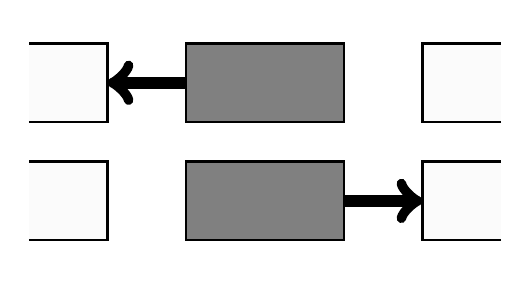
\begin{tikzpicture}
        \path []  (0,-0.2)   -- (0,2.7);       
        
        \draw [thick, fill=gray!3]  (0,1.5) -- (1,1.5) -- (1,2.5) -- (0,2.5);
        \draw [line width=1ex, <-]  (1,2)   -- (2,2);                        
        \draw [thick, fill=gray]    (2,1.5) rectangle (4,2.5);              
        \draw [thick, fill=gray!3]  (6,1.5) -- (5,1.5) -- (5,2.5) -- (6,2.5);

        \draw [thick, fill=gray!3]  (0,0) -- (1,0) -- (1,1) -- (0,1);        
        \draw [thick, fill=gray]    (2,0) rectangle (4,1);                   
        \draw [line width=1ex, ->]  (4,0.5) -- (5,0.5);                      
        \draw [thick, fill=gray!3]  (6,0) -- (5,0) -- (5,1) -- (6,1);
      \end{tikzpicture}
    }} &
    %\multicolumn{1}{m{32em}|}{
    \makecell[l]{ 
    \begin{minipage}[t]{\linewidth}%  
      A cell that will be duplicated in either direction must hold content,
      otherwise a stack underflow exception will be triggered.
    \end{minipage}%
    } \\ \hline

    %SWAP rule
    \multicolumn{1}{|m{3em}|}{
    \makecell[c]{ 
      ``\texttt{SWAP}''\\
      Rule}} &
    \multicolumn{1}{m{7em}|}{
    \scalebox{0.4} {
      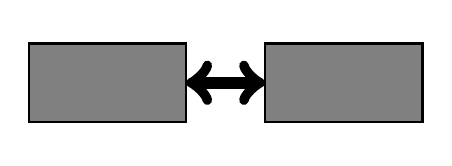
\begin{tikzpicture}
        \path []  (2.25,1.3)   -- (2.25,2.7);       
        
        \draw [thick, fill=gray]     (2.25,1.5) rectangle (4.25,2.5); 
        \draw [line width=1ex, <->]  (4.25,2)   -- (5.25,2);          
        \draw [thick, fill=gray]     (5.25,1.5) rectangle (7.25,2.5); 
      \end{tikzpicture}
    }} &
    %\multicolumn{1}{m{32em}|}{
    \makecell[l]{ 
    \begin{minipage}[t]{\linewidth}%  
      Two neighboring cells that will be swapped must both hold content,
      otherwise a stack underflow exception will be triggered.
    \end{minipage}%
    } \\ \hline

    %Shift rule
    \multicolumn{1}{|m{3em}|}{
    \makecell[c]{ 
      ``Shift''\\
      Rule}} &
    \multicolumn{1}{m{7em}|}{
    \scalebox{0.4} {
      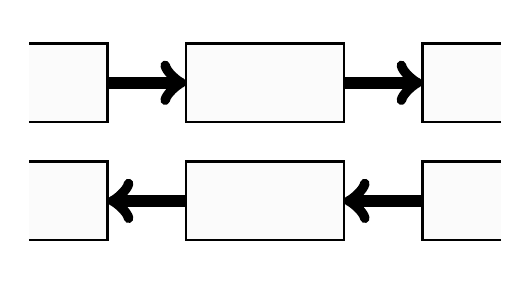
\begin{tikzpicture}
        \path []  (0,-0.2)   -- (0,2.7);       
        
        \draw [thick, fill=gray!3]  (0,1.5) -- (1,1.5) -- (1,2.5) -- (0,2.5);
        \draw [line width=1ex, ->]  (1,2)   -- (2,2);                        
        \draw [thick, fill=gray!3]  (2,1.5) rectangle (4,2.5);              
        \draw [line width=1ex, ->]  (4,2) -- (5,2);                      
        \draw [thick, fill=gray!3]  (6,1.5) -- (5,1.5) -- (5,2.5) -- (6,2.5);

        \draw [thick, fill=gray!3]  (0,0) -- (1,0) -- (1,1) -- (0,1);        
        \draw [line width=1ex, <-]  (1,0.5)   -- (2,0.5);                        
        \draw [thick, fill=gray!3]  (2,0) rectangle (4,1);                   
        \draw [line width=1ex, <-]  (4,0.5) -- (5,0.5);                      
        \draw [thick, fill=gray!3]  (6,0) -- (5,0) -- (5,1) -- (6,1);
      \end{tikzpicture}
    }} &
    %\multicolumn{1}{m{32em}|}{
    \makecell[l]{ 
    \begin{minipage}[t]{\linewidth}%  
      Cells that will be shifted in either direction, will not be checked for content
    \end{minipage}%
    } \\ \hline

    %Cross rule
    \multicolumn{1}{|m{3em}|}{
    \makecell[c]{ 
      ``Cross''\\
      Rule}} &
    \multicolumn{1}{m{7em}|}{
    \scalebox{0.4} {
      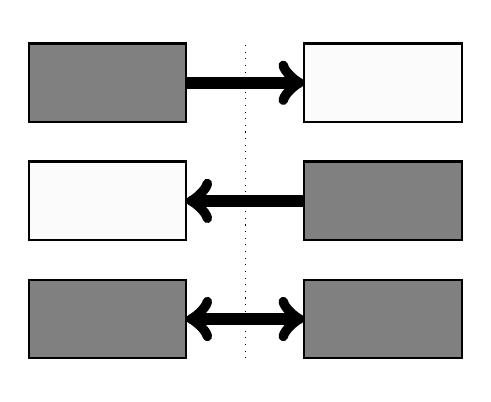
\begin{tikzpicture}

       \path []                      (2,-0.2) --  (2,4.2);             
       \draw [dotted]                (4.75,0) --  (4.75,4);

        \draw [thick, fill=gray]     (2,3) rectangle (4,4); 
        \draw [line width=1ex, ->]   (4,3.5)   -- (5.5,3.5);          
        \draw [thick, fill=gray!3]   (5.5,3) rectangle (7.5,4); 

        \draw [thick, fill=gray!3]   (2,1.5) rectangle (4,2.5); 
        \draw [line width=1ex, <-]   (4,2)   -- (5.5,2);          
        \draw [thick, fill=gray]     (5.5,1.5) rectangle (7.5,2.5); 

        \draw [thick, fill=gray]     (2,0) rectangle (4,1); 
        \draw [line width=1ex, <->]  (4,0.5)   -- (5.5,0.5);          
        \draw [thick, fill=gray]     (5.5,0) rectangle (7.5,1); 

     \end{tikzpicture}
    }} &
    %\multicolumn{1}{m{32em}|}{
    \makecell[l]{ 
    \begin{minipage}[t]{\linewidth}%  
      Any cell that is shifted, swapped or duplicated across the \gls{ps}/\gls{rs} boundary
      must hold content, otherwise a stack underflow exception will be triggered.
    \end{minipage}%
    } \\ \hline

  \end{longtable}
\end{center}  
\endgroup

%Memory Access Instructions
\subsection{Memory Access Instructions}
\label{opcodes:memacc}

Memory access instruction perform read or write acesses to the system's 64K word (128KB) address space.
Data is solely accessed in 16-bit entities.
Accesses to a 255 word (510B) window in the main address space, can be done through an immediate
addressing. This offers faster access to frequently used system variables.

%Function Register access
\subsection{Function Register Access}
\label{opcodes:freg}

The N1 processor provides a set \glspl{freg}, which provide access to a number of processor features
(see \tabref{opcodes:freg:tab}).
These \glspl{freg} are read and written through special \glspl{opcode}.

\begingroup
\setlength{\LTleft}{-20cm plus -1fill}
\setlength{\LTright}{\LTleft}
\begin{center}
  \rowcolors{1}{gray!12}{white}                                         %set alternating row color
  \begin{longtable}{|c|c|c|}
    \rowcolor{white}
    \caption{\Glspl{freg}}
    \label{opcodes:freg:tab} \\
    %Header
    \hline                                     
    \rowcolor{gray!25}
    \multicolumn{1}{|c|}{\textbf{\rule{0pt}{2.5ex}Address}} &  
    \multicolumn{1}{c|}{\textbf{\rule{0pt}{2.5ex}Mnemonic}} &
    \multicolumn{1}{c|}{\textbf{\rule{0pt}{2.5ex}Name}}     \\
    \hline
    \endhead                               
    %Footers
    \hline
    \rowcolor{white}
    \multicolumn{3}{r}{\tiny{...continued}} \\
    \endfoot
    \hline
    \endlastfoot

    %%Carry register (CRY)
    %\texttt{0x00}                               &
    %\hyperref[opcodes:freg:cry]{CRY}            &
    %\hyperref[opcodes:freg:cry]{Carry Register} \\ \hline

    %Parameter Stack Depth Register (PSD)
    \texttt{0x00}                                               &
    \hyperref[opcodes:freg:psd]{PSD}                            &
    \hyperref[opcodes:freg:psd]{Parameter Stack Depth Register} \\ \hline

    %Return Stack Depth Register (PSD)
    \texttt{0x01}                                            &
    \hyperref[opcodes:freg:psd]{RSD}                         &
    \hyperref[opcodes:freg:psd]{Return Stack Depth Register} \\ \hline
    
    %Exception and Interrupt Mask Register (EIM)
    \texttt{0x02}                                                      &
    \hyperref[opcodes:freg:eim]{EIM}                                   &
    \hyperref[opcodes:freg:eim]{Exception and Interrupt Mask Register} \\ \hline

  \end{longtable}
\end{center}  
\endgroup

%%Carry register (CRY)
%\subsubsection{Carry Register (CRY)}
%\label{opcodes:freg:cry}
%
%\begin{figure}[H]
%  %\begin{center}
%  \makebox[\textwidth][c]{
%    %\scalebox{0.5125} {
%    \scalebox{0.515} {
%      \begin{tikzpicture}
%
%        %Offset
%        \node [align=left, anchor=west] at (-2,3) {
%          \huge{Offset: \texttt{0x00}}
%        };        
%        %Index
%        \node [above] at  (1,2) {15};
%        \node [above] at  (3,2) {14};
%        \node [above] at  (5,2) {13};
%        \node [above] at  (7,2) {12};
%        \node [above] at  (9,2) {11};
%        \node [above] at (11,2) {10};
%        \node [above] at (13,2) {9};
%        \node [above] at (15,2) {8};
%        \node [above] at (17,2) {7};
%        \node [above] at (19,2) {6};
%        \node [above] at (21,2) {5};
%        \node [above] at (23,2) {4};
%        \node [above] at (25,2) {3};
%        \node [above] at (27,2) {2};
%        \node [above] at (29,2) {1};
%        \node [above] at (31,2) {0};
%        %Read
%        \node [align=right, anchor=east] at (0,1.5) {\large{Read}};
%        %\draw [thick, fill=white]  (0,1) rectangle (32,2);
%        \draw [thick, fill=gray!3]  (0,1) rectangle  (32,2); %15..0
%        \node at (15,1.5) {\huge{\texttt{CRY}}};
%        %Write
%        \node [align=right, anchor=east] at (0,0.5) {\large{Write}};
%        \draw [thick, fill=white]  (0,0) rectangle (32,1);
%        %\draw [thick, fill=gray!3]  (0,0) rectangle  (32,2); %15..0
%        %\node at (15,0.5) {\huge{\texttt{CRY}}};
%      \end{tikzpicture}
%    }
%  }
%  %\caption{Carry Register}
%  %\label{opcodes:freg:cry:fig}
%  %\end{center}
%\end{figure}
%
%The Carry Register captures the carry or borrow flag of the last addition or suntraction.
%It alwyayread one of the three values:
%\begin{itemize}
%  \item \texttt{1} (carry from the last addition
%  \item \texttt{0} (no carry or borrow)
%  \item \texttt{-1} (borrow from the last subtraction)
%\end{itemize}
%
%\begingroup
%\setlength{\LTleft}{-20cm plus -1fill}
%\setlength{\LTright}{\LTleft}
%\begin{center}
%  \rowcolors{1}{gray!12}{white}                                         %set alternating row color
%  \begin{longtable}{|c|c|c|c|}
%    \rowcolor{white}
%    \caption{Carry  Register Bit Description}
%    \label{opcodes:freg:cry:tab} \\
%    %Header
%    \hline                                     
%    \rowcolor{gray!25}
%    \multicolumn{1}{|c|}{\textbf{\rule{0pt}{2.5ex}Bit}}  &  
%    \multicolumn{1}{c|}{\textbf{\rule{0pt}{2.5ex}Postion}}    & 
%    \multicolumn{1}{c|}{\textbf{\rule{0pt}{2.5ex}Description}} \\
%     \hline
%    \endhead                               
%    %Footers
%    \hline
%    \rowcolor{white}
%    \multicolumn{4}{r}{\tiny{...continued}} \\
%    \endfoot
%    \hline
%    \endlastfoot
%
%    %CRY
%    \texttt{CRY} &
%    15..0        &
%    \multicolumn{1}{m{36em}|}{
%      \makecell[l]{
%        \begin{minipage}[t]{\linewidth}%  
%          \centerline{\textbf{Return Stack Depth}}
%          \begin{description}[style=nextline]
%          \item[Read:]
%            Carry or borrow from last addition or subtraction.\\[1pt]
%          \end{description}
%        \end{minipage}%
%    }}  \\ \hline
%
%  \end{longtable}
%\end{center}  
%\endgroup
%
%~\\

%Parameter Stack Depth Reggister (PSD)
\subsubsection{Parameter Stack Depth Register (PSD)}
\label{opcodes:freg:psd}

\begin{figure}[H]
  %\begin{center}
  \makebox[\textwidth][c]{
    %\scalebox{0.5125} {
    \scalebox{0.515} {
      \begin{tikzpicture}

        %Offset
        \node [align=left, anchor=west] at (-2,3) {
          \huge{Offset: \texttt{0x00}}
        };        
        %Index
        \node [above] at  (1,2) {15};
        \node [above] at  (3,2) {14};
        \node [above] at  (5,2) {13};
        \node [above] at  (7,2) {12};
        \node [above] at  (9,2) {11};
        \node [above] at (11,2) {10};
        \node [above] at (13,2) {9};
        \node [above] at (15,2) {8};
        \node [above] at (17,2) {7};
        \node [above] at (19,2) {6};
        \node [above] at (21,2) {5};
        \node [above] at (23,2) {4};
        \node [above] at (25,2) {3};
        \node [above] at (27,2) {2};
        \node [above] at (29,2) {1};
        \node [above] at (31,2) {0};
        %Read
        \node [align=right, anchor=east] at (0,1.5) {\large{Read}};
        %\draw [thick, fill=white]  (0,1) rectangle (32,2);
        \draw [thick, fill=gray!3]  (0,1) rectangle  (32,2); %15..0
        \node at (15,1.5) {\huge{\texttt{PSD}}};
        %Write
        \node [align=right, anchor=east] at (0,0.5) {\large{Write}};
        %\draw [thick, fill=white]  (0,0) rectangle (32,1);
        \draw [thick, fill=gray!3]  (0,0) rectangle  (32,1); %15..0
        \node at (15,0.5) {\huge{\texttt{PSDCLR}}};
      \end{tikzpicture}
    }
  }
  %\caption{Parameter Stack Depth Register}
  %\label{opcodes:freg:psd:fig}
  %\end{center}
\end{figure}

The current depth of the \gls{ps} is captured in the parameter stack depth register. \\
Writing \texttt{0x0000} to this register will clear the \gls{ps}.

\begingroup
\setlength{\LTleft}{-20cm plus -1fill}
\setlength{\LTright}{\LTleft}
\begin{center}
  \rowcolors{1}{gray!12}{white}                                         %set alternating row color
  \begin{longtable}{|c|c|c|c|}
    \rowcolor{white}
    \caption{Parameter Stack Depth Register Bit Description}
    \label{opcodes:freg:psd:tab} \\
    %Header
    \hline                                     
    \rowcolor{gray!25}
    \multicolumn{1}{|c|}{\textbf{\rule{0pt}{2.5ex}Bit}}  &  
    \multicolumn{1}{c|}{\textbf{\rule{0pt}{2.5ex}Postion}}    & 
    \multicolumn{1}{c|}{\textbf{\rule{0pt}{2.5ex}Description}} \\
     \hline
    \endhead                               
    %Footers
    \hline
    \rowcolor{white}
    \multicolumn{4}{r}{\tiny{...continued}} \\
    \endfoot
    \hline
    \endlastfoot

    %PSD
    \texttt{PSD} &
    15..0        &
    \multicolumn{1}{m{36em}|}{
      \makecell[l]{
        \begin{minipage}[t]{\linewidth}%  
          \centerline{\textbf{Parameter Stack Depth}}
          \begin{description}[style=nextline]
          \item[Read:]
            Current parameter stack depth\\[1pt]
          \end{description}
        \end{minipage}%
    }}  \\ \hline

    %PSDCLR
    \texttt{PSDCLR} &
    15..0        &
    \multicolumn{1}{m{36em}|}{
      \makecell[l]{
        \begin{minipage}[t]{\linewidth}%  
          \centerline{\textbf{Clear Parameter Stack}}
          \begin{description}[style=nextline]
          \item[Write:]
            Writing the value \texttt{0x0000} will clrear the \gls{ps}.\\
            All other write accesses have no effect.\\[1pt]
          \end{description}
        \end{minipage}%
    }}  \\ \hline
 
  \end{longtable}
\end{center}  
\endgroup

~\\

%Return Stack Depth Register (RSD)
\subsubsection{Return Stack Depth Register (RSD}
\label{opcodes:freg:rsd}

\begin{figure}[H]
  %\begin{center}
  \makebox[\textwidth][c]{
    %\scalebox{0.5125} {
    \scalebox{0.515} {
      \begin{tikzpicture}

        %Offset
        \node [align=left, anchor=west] at (-2,3) {
          \huge{Offset: \texttt{0x01}}
        };        
        %Index
        \node [above] at  (1,2) {15};
        \node [above] at  (3,2) {14};
        \node [above] at  (5,2) {13};
        \node [above] at  (7,2) {12};
        \node [above] at  (9,2) {11};
        \node [above] at (11,2) {10};
        \node [above] at (13,2) {9};
        \node [above] at (15,2) {8};
        \node [above] at (17,2) {7};
        \node [above] at (19,2) {6};
        \node [above] at (21,2) {5};
        \node [above] at (23,2) {4};
        \node [above] at (25,2) {3};
        \node [above] at (27,2) {2};
        \node [above] at (29,2) {1};
        \node [above] at (31,2) {0};
        %Read
        \node [align=right, anchor=east] at (0,1.5) {\large{Read}};
        %\draw [thick, fill=white]  (0,1) rectangle (32,2);
        \draw [thick, fill=gray!3]  (0,1) rectangle  (32,2); %15..0
        \node at (15,1.5) {\huge{\texttt{RSP}}};
        %Write
        \node [align=right, anchor=east] at (0,0.5) {\large{Write}};
        %\draw [thick, fill=white]  (0,0) rectangle (32,1);
        \draw [thick, fill=gray!3]  (0,0) rectangle  (32,1); %15..0
        \node at (15,0.5) {\huge{\texttt{RSPCLR}}};
      \end{tikzpicture}
    }
  }
  %\caption{Return Stack Depth Register}
  %\label{opcodes:freg:rsd:fig}
  %\end{center}
\end{figure}

The current depth of the \gls{rs} is captured in the parameter stack depth register. \\
Writing \texttt{0x0000} to this register will clear the \gls{rs}.

\begingroup
\setlength{\LTleft}{-20cm plus -1fill}
\setlength{\LTright}{\LTleft}
\begin{center}
  \rowcolors{1}{gray!12}{white}                                         %set alternating row color
  \begin{longtable}{|c|c|c|c|}
    \rowcolor{white}
    \caption{Return Stack Depth Register Bit Description}
    \label{opcodes:freg:rsd:tab} \\
    %Header
    \hline                                     
    \rowcolor{gray!25}
    \multicolumn{1}{|c|}{\textbf{\rule{0pt}{2.5ex}Bit}}  &  
    \multicolumn{1}{c|}{\textbf{\rule{0pt}{2.5ex}Postion}}    & 
    \multicolumn{1}{c|}{\textbf{\rule{0pt}{2.5ex}Description}} \\
     \hline
    \endhead                               
    %Footers
    \hline
    \rowcolor{white}
    \multicolumn{4}{r}{\tiny{...continued}} \\
    \endfoot
    \hline
    \endlastfoot

    %RSD
    \texttt{RSD} &
    15..0        &
    \multicolumn{1}{m{36em}|}{
      \makecell[l]{
        \begin{minipage}[t]{\linewidth}%  
          \centerline{\textbf{Return Stack Depth}}
          \begin{description}[style=nextline]
          \item[Read:]
            Current return stack depth.\\[1pt]
          \end{description}
        \end{minipage}%
    }}  \\ \hline

    %RSDCLR
    \texttt{RSDCLR} &
    15..0        &
    \multicolumn{1}{m{36em}|}{
      \makecell[l]{
        \begin{minipage}[t]{\linewidth}%  
          \centerline{\textbf{Return Stack Depth}}
          \begin{description}[style=nextline]
          \item[Write:]
            Writing the value \texttt{0x0000} will clrear the \gls{rs}.\\
            All other write accesses have no effect.\\[1pt]
          \end{description}
        \end{minipage}%
    }}  \\ \hline

  \end{longtable}
\end{center}  
\endgroup

~\\

%Exception and Interrupt Mask Register (EIM)
\subsubsection{Exception and Interrupt Mask Register (EIM)}
\label{opcodes:freg:eim}

\begin{figure}[H]
  %\begin{center}
  \makebox[\textwidth][c]{
    %\scalebox{0.5125} {
    \scalebox{0.515} {
      \begin{tikzpicture}

        %Offset
        \node [align=left, anchor=west] at (-2,3) {
          \huge{Offset: \texttt{0x02}}
        };        
        %Index
        \node [above] at  (1,2) {15};
        \node [above] at  (3,2) {14};
        \node [above] at  (5,2) {13};
        \node [above] at  (7,2) {12};
        \node [above] at  (9,2) {11};
        \node [above] at (11,2) {10};
        \node [above] at (13,2)  {9};
        \node [above] at (15,2)  {8};
        \node [above] at (17,2)  {7};
        \node [above] at (19,2)  {6};
        \node [above] at (21,2)  {5};
        \node [above] at (23,2)  {4};
        \node [above] at (25,2)  {3};
        \node [above] at (27,2)  {2};
        \node [above] at (29,2)  {1};
        \node [above] at (31,2)  {0};
        %Read
        \node [align=right, anchor=east] at (0,1.5) {\large{Read}};
        \draw [thick, fill=white] (0,1) rectangle (32,2);
        \node at ( 1,1.5) {\huge{\texttt{0}}};               %15
        \node at ( 3,1.5) {\huge{\texttt{0}}};               %14
        \node at ( 5,1.5) {\huge{\texttt{0}}};               %13
        \node at ( 7,1.5) {\huge{\texttt{0}}};               %12
        \node at ( 9,1.5) {\huge{\texttt{0}}};               %11
        \node at (11,1.5) {\huge{\texttt{0}}};               %10
        \node at (13,1.5) {\huge{\texttt{0}}};               % 9
        \node at (15,1.5) {\huge{\texttt{0}}};               % 8
        \node at (17,1.5) {\huge{\texttt{0}}};               % 7
        \node at (19,1.5) {\huge{\texttt{0}}};               % 6
        \node at (21,1.5) {\huge{\texttt{0}}};               % 5
        \node at (23,1.5) {\huge{\texttt{0}}};               % 4
        \node at (25,1.5) {\huge{\texttt{0}}};               % 3
        \node at (29,1.5) {\huge{\texttt{0}}};               % 1
        %Write
        \node [align=right, anchor=east] at (0,0.5) {\large{Write}};
        \draw [thick, fill=white] (0,0) rectangle (32,1);
        \draw [thick, fill=gray!3] (24,0) rectangle (26,1);  % 3
        \node at (25,0.5) {\Large{\texttt{EMWE}}};
        \draw [thick, fill=gray!3] (26,0) rectangle (28,2);  % 2
        \node at (27,1)   {\Large{\texttt{EM}}};
        \draw [thick, fill=gray!3] (28,0) rectangle (30,1);  % 1
        \node at (29,0.5) {\Large{\texttt{IMWE}}};
        \draw [thick, fill=gray!3] (30,0) rectangle (32,2);  % 0
        \node at (31,1)   {\Large{\texttt{IM}}};
        \end{tikzpicture}
    }
  }
  %\caption{Interrupt and Exception Enable Register}
  %\label{opcodes:freg:eim:fig}
  %\end{center}
\end{figure}

Interrupt and exception handling can be disabled through two control register bits:
\texttt{IM} (interrupt mask) and \texttt{EM} (exception mask).
This is to avoid \gls{rs} overflows, caused by nested execution of exceptions and interrupt sevice routines.

The \texttt{IM} bit is automatically set when an interrupt service routine is started.
The \texttt{eM} bit is automatically set when an exception handler is executed.
Both flags mut be set manually as soon as new interrupts or exceptions can be processed.
Each one of these bits is protected by a write enable bit to atomic bit manipulations.

\begingroup
\setlength{\LTleft}{-20cm plus -1fill}
\setlength{\LTright}{\LTleft}
\begin{center}
  \rowcolors{1}{gray!12}{white}                                         %set alternating row color
  \begin{longtable}{|c|c|c|c|}
    \rowcolor{white}
    \caption{Exception and Interrupt Mask Register Bit Description}
    \label{opcodes:freg:eim:tab} \\
    %Header
    \hline                                     
    \rowcolor{gray!25}
    \multicolumn{1}{|c|}{\textbf{\rule{0pt}{2.5ex}Bit}}       &  
    \multicolumn{1}{c|}{\textbf{\rule{0pt}{2.5ex}Postion}}    & 
    \multicolumn{1}{c|}{\textbf{\rule{0pt}{2.5ex}Description}} \\
     \hline
    \endhead                               
    %Footers
    \hline
    \rowcolor{white}
    \multicolumn{4}{r}{\tiny{...continued}} \\
    \endfoot
    \hline
    \endlastfoot

    %EMWE
    \texttt{EMWE} &
    3               &
    \multicolumn{1}{m{36em}|}{
      \makecell[l]{
        \begin{minipage}[t]{\linewidth}%  
          \centerline{\textbf{Exception Mask Write Enable}}
          \begin{description}[style=nextline]
          %\item[Read:]
          %  Always reads zero.
          \item[Write:]
            Writing a \texttt{1} allows modification of the \texttt{EM} bit in the same access.\\[1pt]
          \end{description}
        \end{minipage}%
    }}  \\ \hline
    
   %EM
   \texttt{EM} &
   2               &
   \multicolumn{1}{m{36em}|}{
   \makecell[l]{ 
     \begin{minipage}[t]{\linewidth}%  
     \centerline{\textbf{Exception Mask}}
     \begin{description}[style=nextline]
     \item[Read:]
     \begin{minipage}[t]{\linewidth}  
       \begin{description}[style=multiline]
         \item[\texttt{0}:]
           Exceptions are enabled.
         \item[\texttt{1}:]
           Exceptions are disbled.
         \end{description}
     \end{minipage}
     \item[Write:]
     \begin{minipage}[t]{\linewidth}
       \begin{description}[style=multiline]
         \item[\texttt{0}:]
            Disable exceptions. Only possible while instantly writing a \texttt{1} to \texttt{EMWE}. 
         \item[\texttt{1}:]
           Disable exceptions. Only possible while instantly writing a \texttt{1} to \texttt{EMWE}.\\[1pt]
       \end{description}
     \end{minipage}  
     \end{description}
     \end{minipage}%
   }}  \\ \hline
   
    %IMWE
    \texttt{IMWE} &
    1               &
    \multicolumn{1}{m{36em}|}{
      \makecell[l]{
        \begin{minipage}[t]{\linewidth}%  
          \centerline{\textbf{Interrupt Mask Write Enable}}
          \begin{description}[style=nextline]
          %\item[Read:]
          %  Always reads zero.
          \item[Write:]
            Writing a \texttt{1} allows modification of the \texttt{IM} bit in the same access.\\[1pt]
          \end{description}
        \end{minipage}%
    }}  \\ \hline
    
   %IM
   \texttt{IEN} &
   0               &
   \multicolumn{1}{m{36em}|}{
   \makecell[l]{ 
     \begin{minipage}[t]{\linewidth}%  
     \centerline{\textbf{Interrupt Mask}}
     \begin{description}[style=nextline]
     \item[Read:]
     \begin{minipage}[t]{\linewidth}  
       \begin{description}[style=multiline]
         \item[\texttt{0}:]
           Interrupts are enabled.
         \item[\texttt{1}:]
           Interrupts are disabled.
         \end{description}
     \end{minipage}
     \item[Write:]
     \begin{minipage}[t]{\linewidth}
       \begin{description}[style=multiline]
         \item[\texttt{0}:]
            Disable interrupts. Only possible while instantly writing a \texttt{1} to \texttt{IMWE}. 
         \item[\texttt{1}:]
           Disable interrupts. Only possible while instantly writing a \texttt{1} to \texttt{IMWE}.\\[1pt]
       \end{description}
     \end{minipage}  
     \end{description}
     \end{minipage}%
   }}  \\ \hline
   
  \end{longtable}
\end{center}  
\endgroup



%--------------------
% N1 integration parameters
%--------------------
%\include{N1_parameters}

%--------------------
% N1 interface signals
%--------------------
%\include{N1_signals}

%--------------------
% N1 components
%--------------------
%\include{N1_components}

%--------------------
% Verification 
%--------------------
%%###############################################################################
%# N1 - Manual - Verification Status                                           #
%###############################################################################
%#    Copyright 2018 - 2019 Dirk Heisswolf                                     #
%#    This file is part of the N1 project.                                     #
%#                                                                             #
%#    N1 is free software: you can redistribute it and/or modify               #
%#    it under the terms of the GNU General Public License as published by     #
%#    the Free Software Foundation, either version 3 of the License, or        #
%#    (at your option) any later version.                                      #
%#                                                                             #
%#    N1 is distributed in the hope that it will be useful,                    #
%#    but WITHOUT ANY WARRANTY; without even the implied warranty of           #
%#    MERCHANTABILITY or FITNESS FOR A PARTICULAR PURPOSE.  See the            #
%#    GNU General Public License for more details.                             #
%#                                                                             #
%#    You should have received a copy of the GNU General Public License        #
%#    along with N1.  If not, see <http://www.gnu.org/licenses/>.              #
%###############################################################################
%# Version History:                                                            #
%#   March 4, 2019                                                             #
%#      - Initial release                                                      #
%###############################################################################

\section{Verification Status}
\label{verification}

TBD



%--------------------
% Tool summary
%--------------------
%%###############################################################################
%# N1 - Manual - Tool Summary                                                  #
%###############################################################################
%#    Copyright 2018 - 2019 Dirk Heisswolf                                     #
%#    This file is part of the N1 project.                                     #
%#                                                                             #
%#    N1 is free software: you can redistribute it and/or modify               #
%#    it under the terms of the GNU General Public License as published by     #
%#    the Free Software Foundation, either version 3 of the License, or        #
%#    (at your option) any later version.                                      #
%#                                                                             #
%#    N1 is distributed in the hope that it will be useful,                    #
%#    but WITHOUT ANY WARRANTY; without even the implied warranty of           #
%#    MERCHANTABILITY or FITNESS FOR A PARTICULAR PURPOSE.  See the            #
%#    GNU General Public License for more details.                             #
%#                                                                             #
%#    You should have received a copy of the GNU General Public License        #
%#    along with N1.  If not, see <http://www.gnu.org/licenses/>.              #
%###############################################################################
%# Version History:                                                            #
%#   March 5, 2019                                                             #
%#      - Initial release                                                      #
%###############################################################################

\section{Tool Summary}
\label{tools}

TBD



%--------------------
% Bibliography
%--------------------
\bibliographystyle{plain}
\bibliography{N1.bib}

\end{document}
